\documentclass[12pt]{article}
\usepackage{graphicx,psfrag,epsf}
\usepackage{enumerate}
\usepackage{natbib}
\usepackage{amsfonts}
\usepackage{amsmath}
\usepackage{float}
\usepackage{amsthm}
\usepackage{xcolor}
\usepackage{amssymb,mathabx}
\usepackage{algorithm, algpseudocode}
\usepackage[utf8]{inputenc}
\usepackage[english]{babel}
\newtheorem{theorem}{Theorem}
\newtheorem{lemma}[theorem]{Lemma}
\newtheorem{proposition}[theorem]{Proposition}
\newcommand{\blind}{0}
\addtolength{\oddsidemargin}{-.75in}%
\addtolength{\evensidemargin}{-.75in}%
\addtolength{\textwidth}{1.5in}%
\addtolength{\textheight}{1.3in}%
\addtolength{\topmargin}{-.8in}%

% formatting tweaks
\newcommand{\te}{\!=\!} % thin equals
\newcommand{\tneq}{\!\neq\!}
\newcommand{\naive}{na\"{\i}ve}
\newcommand{\Naive}{Na\"{\i}ve}
\newcommand{\Levy}{L\'{e}vy}
\newcommand{\myvcenter}[1]{\ensuremath{\vcenter{\hbox{#1}}}} % vertical centering

% bold and caligraphic letters
\newcommand{\ba}{\mathbf{a}}
\newcommand{\bb}{\mathbf{b}}
\newcommand{\bc}{\mathbf{c}}
\newcommand{\bd}{\mathbf{d}}
\newcommand{\bg}{\mathbf{g}}
\newcommand{\bh}{\mathbf{h}}
\newcommand{\bs}{\mathbf{s}}
\newcommand{\bu}{\mathbf{u}}
\newcommand{\bw}{\mathbf{w}}
\newcommand{\bx}{\mathbf{x}}
\newcommand{\by}{\mathbf{y}}
\newcommand{\hyp}{{\mathcal H}}
\newcommand{\model}{{\mathcal M}}
\newcommand{\data}{{\mathcal D}}
\newcommand{\Z}{{\mathcal Z}}
\newcommand{\N}{{\mathcal N}}
\newcommand{\M}{{\mathcal M}}
\newcommand{\F}{{\mathcal F}}
\newcommand{\vS}{{\vec{S}}}
\newcommand{\cS}{{\mathcal S}}
\newcommand{\vcS}{{\vec{\mathcal S}}}
\newcommand{\cT}{{\mathcal T}}
\newcommand{\cN}{{\mathcal N}}
\newcommand{\cV}{{\mathcal V}}
\newcommand{\ocS}{\overline{\mathcal S}}
\newcommand{\Tu}{\mathcal{T}^{\cup}}
\newcommand{\Su}{\mathcal{S}^{\cup}}
\newcommand{\vSu}{\vec{\mathcal{S}}^{\cup}}
\newcommand{\Mu}{\mathcal{M}^{\cup}}
\newcommand{\muu}{\mu^{\cup}}
\newcommand{\vmuu}{\vec{\mu}^{\cup}}
\newcommand{\mul}{\mu^{<}}
\newcommand{\tmuu}{\tilde{\mu}^{\cup}}
\newcommand{\oSigma}{\overline{\Sigma}}
\newcommand{\vSigma}{\vec{\Sigma}}
\newcommand{\dif}{\mathrm{d}}

% arrows without lots of space
\newcommand{\la}{\!\leftarrow\!}
\newcommand{\ra}{\!\rightarrow\!}
\newcommand{\lra}{\!\leftrightarrow\!}

\newcommand{\fwd}{\mathtt{f}}
\newcommand{\bck}{\mathtt{b}}

% Miscellaneous mathematics
\newcommand{\nth}{^{\left( n \right)}}
\newcommand{\mth}{^{\left( m \right)}}
\newcommand{\nnth}[1]{^{\left(#1\right)}}
\DeclareMathOperator*{\argmax}{argmax}
\DeclareMathOperator*{\argmin}{argmin}
\newcommand{\pdd}[2]{\frac{\partial #1}{\partial #2}}

% Colors
%\usepackage{color}

\newcommand{\txss}{\textsuperscript}
 \newcommand{\defeq}{\stackrel{\textup{\tiny def}}{=}}

% defined again below
%\def\l({\left(}
%\def\r){\right)}



\DeclareMathOperator*{\KL}{KL}

\def\bS{\mathbf{S}}
\def\tbS{\tilde{\bS}}
\def\tS{\tilde{S}}
\def\ts{\tilde{s}}
\def\tt{\tilde{t}}
\def\tT{\tilde{T}}
\def\tA{\tilde{A}}
\def\tI{\tilde{I}}
\def\tP{\tilde{P}}
\def\tR{\tilde{R}}
\def\tW{\tilde{W}}
\def\tw{\tilde{w}}
\def\tF{\tilde{F}}
\def\tG{\tilde{G}}
\def\tE{\tilde{E}}
\def\bL{\mathbf{L}}
\def\E{E}
%\newcommand{\mW}{{\mathcal W}}
\newcommand{\mW}{{|W^\downarrow}|}
\newcommand{\assign}{\doteq}

\def\ind{1}

\newcommand{\avg}[1]{\langle{#1} \rangle}

\def\naive{na\"{\i}ve}
\def\hlambda{\hat{\lambda}}
\def\ulmb{\underline{\lambda}}
\def\olmb{\overline{\lambda}}
\def\uR{\underline{R}}
\def\oR{\overline{R}}
\def\Reps{R^{\epsilon}}
\def\leps{\lambda^{\epsilon}}

% these break default latex commands for, e.g., Swedish names
%\def\l({\left(} 
%\def\r){\right)}

\def\matern{Mat\'{e}rn }

\newcommand{\NOTE}[1]{\textcolor{red}{[#1]}}
\newcommand{\vinayak}[1]{\textcolor{red}{[Vinayak: #1]}}
\newcommand{\boqian}[1]{\textcolor{blue}{[Boqian: #1]}}
\newcommand{\given}{\,|\,}

\newcommand{\PP}{\text{PoissProc}}
\newcommand{\from}{\text{ from }}
\newcommand{\Mx}[1]{{\max_s |A_s(#1)|}}
\newcommand{\mx}[1]{{\min_s |A_s(#1)|}}

\newcommand{\SM}{B}
\newcommand\numberthis{\addtocounter{equation}{1}\tag{\theequation}}

\newcommand{\lb}{\ell}
\newcommand{\ub}{u}
\newcommand{\algname}{Rao-Teh}
\def\ctheta{\theta}
\def\ntheta{\theta'}
%\def\ptheta{\theta^{*}}
\def\ptheta{\nu}
\newcommand{\prior}{P}


\begin{document}


%\bibliographystyle{plain}

\def\spacingset#1{\renewcommand{\baselinestretch}%
{#1}\small\normalsize} \spacingset{1}


%%%%%%%%%%%%%%%%%%%%%%%%%%%%%%%%%%%%%%%%%%%%%%%%%%%%%%%%%%%%%%%%%%%%%%%%%%%%%%

\if0\blind
{
  \title{\bf Efficient MCMC for parameter inference for Markov jump processes}
  \author{  
   %  Vinayak Rao\thanks{
    %The authors gratefully acknowledge}\hspace{.2cm}\\
    %Department of Statistics, Purdue University\\
    %and \\
    Boqian Zhang \\
    Department of Statistics, Purdue University\\
    Vinayak Rao\\
    Department of Statistics, Purdue University\\
    }
  \maketitle
} \fi

\if1\blind
{
  \bigskip
  \bigskip
  \bigskip
  \begin{center}
    {\LARGE\bf Title}
\end{center}
  \medskip
} \fi

\bigskip
\begin{abstract}
Markov jump processes (MJPs) are continuous-time stochastic processes that 
find wide application in a variety of fields.  Inference for MJPs typically proceeds via Markov chain Monte Carlo, 
the state-of-the-art being an auxiliary variable Gibbs sampler proposed recently
in~\cite{RaoTeh13}. This algorithm was designed for the situation where
the MJP parameters are known, and Bayesian inference over unknown parameters
is typically carried out by incorporating this into a larger Gibbs 
sampler. %In many situations, the MJP trajectory and parameters can exhibit
%strong coupling, and 
This strategy of alternately sampling parameters given path, and 
then path given parameters can result in poor mixing. In this 
work, we propose a simple and elegant algorithm to address this 
problem. Our scheme brings Metropolis-Hastings (MH) approaches 
for discrete-time hidden Markov models (HMMs) to the continuous-time
setting, and also also ties up some of the loose ends 
in~\cite{RaoTeh13}. The result is a complete and clean recipe for 
parameter and path inference in MJPs. In our experiments, we 
demonstrate superior performance over Gibbs sampling, as well as 
other approaches like particle Markov chain Monte 
Carlo~\cite{Andrieu10}.
\end{abstract}
\noindent%
{\it Keywords:}  Markov jump process, MCMC, Metropolis-Hasting, Bayesian inference

\spacingset{1.45}

\section{Introduction}
\label{sec:intro}
Markov jump processes (MJPs) are continuous-time stochastic processes widely used in fields like computational chemistry~\citep{gillespie97}, molecular genetics~\citep{FearnSher2006}, mathematical finance~\citep{Elliott06}, queuing theory~\citep{Breuer2003}, artificial intelligence~\citep{XuShe10} and social-network analysis~\citep{pan2016markov}. 
MJPs have been used as realistic, mechanistic and interpretable models of a wide variety of phenomena, among others, the references above have used them to model temporal evolution of the state of a chemical reaction or queuing network, segmentation of a strand of DNA, and user activity on social media.
Their continuous-time dynamics however raise computational challenges when, given noisy measurements, one wants to make inferences 
over the latent MJP trajectory as well as any process parameters. 
In contrast to {discrete-time} hidden Markov models, one cannot 
{\em a priori} bound the number of trajectory state transitions, and the transition times themselves are continuous-valued. 
The state-of-the-art approach is an auxiliary variable Gibbs sampler from~\cite{RaoTeh13}, we will refer to this as the {\algname} algorithm. 
This Markov chain Monte Carlo (MCMC) algorithm was designed to simulate paths when the MJP parameters are known. 
Parameter inference is typically carried out by incorporating it into a Gibbs sampler that also conditionally simulates parameters given the currently sampled trajectory. 

In many situations, the MJP trajectory and parameters exhibit strong coupling, so that alternately sampling path given parameters, and parameters given path can result in poor mixing.  
To address this, we propose an efficient Metropolis-Hastings (MH) sampler (algorithm~\ref{alg:MH_improved}). 
%additionally, we tie up some of the loose ends in the Rao-Teh algorithm.
In our experiments, we demonstrate superior performance over Gibbs sampling, a more \naive\ MH sampler, as well as particle Markov chain Monte Carlo~\citep{Andrieu10}. 
We also prove that under relatively mild conditions, our sampler inherits geometric ergodicity from an `ideal' sampler that is computationally much more expensive.

\section{Markov jump processes (MJPs)} 
\label{sec:mjp}
A Markov jump process~\citep{Cinlar1975} is a right-continuous piecewise-constant stochastic process $S(t)$ taking values in a state space $\cS$. % (see Figure~\ref{fig:naive_mh}, top-left).
We assume a finite number of states $N$, with $\cS = \{1,\ldots,N\}$. 
Then, the MJP is parameterized by two quantities, an $N$-component probability vector $\pi_0$ and a rate-matrix $A$. 
The former gives the distribution over states at the initial time (we assume this is $0$), while the latter is an $N \times N$-matrix governing the dynamics of the system.  
An off-diagonal element $A_{ij}$ gives the rate of transitioning from state $i$ to $j$. 
The rows of $A$ sum to $0$, so that $A_{ii}=-\sum_{j \neq i} A_{ij}  $. 
We write $A_i$ for the negative of the $i$th diagonal element $A_{ii}$, so that $A_i = -A_{ii}$ gives the total rate at which the system leaves state $i$ for any other state.
To simulate an MJP over an interval $[0,t_{end})$, one follows Gillespie's algorithm~\citep{gillespie97}: 
first sample an initial state $s_0$ from $\pi_0$, and defining $t_0 = t_{curr} = 0$ and $k = 0$, repeat the following while $t_{curr} < t_{end}$:
\begin{itemize}
  \item Sample a wait-time $\Delta t_k$ from an exponential distribution with rate $A_{s_k}$.  
    Set $t_{k+1} = t_{curr} = t_{k} + \Delta t_k$. 
    The MJP remains in state $s_k$ until time $t_{k+1}$.
  \item Jump to a new state $s_{k+1} \neq s_k$ with probability equal to $A_{s_ks_{k+1}}/A_{s_k}$. Set $k=k+1$.
\end{itemize}
The times $T=(t_1, \dotsc, t_{k - 1})$ and states $S=(s_1, \dotsc, s_{k - 1 })$, along with the initial state $s_0$, define the MJP path, so that $\{S(t), t \in [0,t_{end})\} \equiv (s_0, S,T)$. 
See the top-left panel in figure~\ref{fig:MH_improved} for a sample path.

\vspace{-.15in}
\subsection{Structured rate matrices}
While the rate matrix $A$ can have $N(N-1)$ independent elements, in typical applications, especially with large state-spaces, it is determined by a much smaller set of parameters. 
We will write these as $\theta$, with $A$ a deterministic function of these parameters: $A \equiv A(\theta)$. 
The parameters $\theta$ are often more interpretable than the elements of $A$,and correspond directly to physical, biological or environmental parameters of interest. 
For example:
\begin{description}
  \item[Immigration-death processes] 
    Here, $\theta = (\alpha,\beta)$, with $\alpha$ the arrival-rate and $\beta$ the death-rate. 
    The state represents the size of a population or queue. 
    New individuals enter with rate $\alpha$, so off-diagonal elements $A_{i,i+1}$ equal $\alpha$.
    Each individual dies at a rate $\beta$, so that $A_{i,i-1}=i\beta$.
    All other transitions have rate $0$. 
   % so that $\theta = (\alpha,\beta)$,
   % and $A(\theta)$ is tri-diagonal.
  \item[Birth-death processes] 
    This variant of the earlier MJP moves from state $i$ to $i+1$ with rate $i\alpha$, with growth-rate is proportional to population size. 
    Again, the death-rate is $\beta$, so that $A_{i,i-1}=i\beta$.
    The other off-diagonal elements are $0$, and again $\theta=(\alpha,\beta)$.
  \item[Codon substitution models] 
    These characterize transitions between codons at a DNA locus over evolutionary time. 
    There are $61$ codons, and in the simplest case, all transitions have the same rate~\citep{jukescantor69}: $A_{ij} = \alpha\ \forall i \neq j$. 
    Thus the $61\times 61$ matrix $A$ is determined by a single $\alpha$. 
    Other models~\citep{goldman1994codon} group transitions as `synonymous' and `nonsynonymous', based on whether old and new codons encode the same amino acid. 
    Synonymous and nonsynonymous transitions have their own rates, so $A$ is determined by 2 parameters $\alpha$ and $\beta$. 
  %  More refined models~\citep{goldman1994codon} introduce additional structure and parameters. 
    %however the 
    %number of parameters is still significantly smaller than the general case.
\end{description}

\section{Bayesian modeling and inference for MJPs}
\label{sec:bayes_model}
%In practical situations, an MJP is noisily observed at
%a finite set of times. %with the observations themselves noisy. 
%This raises two questions: 
%%\begin{itemize}
%1) what is the underlying trajectory? and 2%)
%  what are the MJP parameters?
%%\end{itemize}
%  \vspace{-.1in}
%\textbf{Bayesian model:}
We first set up our Bayesian model of the data generation process. 
We model a latent piecewise-constant path $S(t)$ as an $N$-state MJP with rate matrix $A(\theta)$ and prior $\pi_0$ over $S(0)$, the state at time $0$. 
The parameter $\theta$ is unknown, and we place a prior $\prior(\theta)$ over this. 
For clarity we will assume $\pi_0$ is known (or we set it to a uniform distribution over the $N$ states). 
In settings with multiple trajectories, we would place a Dirichlet prior over $\pi_0$. 
We have noisy measurements $X$ of $S(t)$, with likelihood $P(X|\{S(t),\ t \in [0,t_{end}]\})$.
Again, for clarity we ignore any unknown parameters in the likelihood, otherwise we could include them in $\theta$.
We assume the observation process has the following structure: for any partition $W = \{w_0 = 0, w_1, \dotsc, w_{|W|}=t_{end}\}$ of the interval $[0,t_{end}]$, there exist known functions $\ell_i$ such that the likelihood factors as:
\begin{align}
  \label{eq:lik_factor}
  P(X|\{S(t),\ t \in [0,t_{end}]\}) = \prod_{i=0}^{|W|-1} \ell_i(\{S(t),\ t \in [w_{i},w_{i+1})\})
\end{align}
A common example where this holds is for observations $X$ at a finite set of times $T^X = \{t^X_1,\cdots, t^X_{|X|}\}$, each observation depending on the state of the MJP at that time:
\begin{align}
  \label{eq:lik_iid}
  P(X|\{S(t),\ t \in [0,t_{end}]\}) = \prod_{i=1}^{|X|} P(x_i|S(t^X_i)).
\end{align}
Other examples include settings when the observations form an inhomogeneous Poisson process~\citep{FearnSher2006}, renewal process~\citep{rao2011gaussian} or even another MJP~\citep{Nodelman+al:UAI02,RaoTeh13}, modulated by $S(t)$.
The first example, called a Markov modulated Poisson process (MMPP)~\citep{scottmmpp03}, associates a positive rate $\lambda_s$ with each state $s$, with $\ell_i(\{S(t),\ t \in [w_{i},w_{i+1})\})$ equal to the likelihood of the Poisson events within $[w_{i-1},w_i]$ under an inhomogeneous Poisson process with piecewise-constant rate $\lambda_{S(t)},\ t \in [w_{i},w_{i+1}]$.

With $A(\cdot)$ and $\pi_0$ assumed known, the overall Bayesian model is then 
\begin{align}
  \label{eq:bayes_model}
  \theta \sim P(\theta), \quad S(t) \sim \text{MJP}(A(\theta), \pi_0), \quad X \sim P(X|\{S(t),\ t \in [0,t_{end}]\}).
\end{align}
Given $X$, one is interested in the posterior distribution over the latent quantities, $(\theta,S(t))$. 

\subsection{Trajectory inference given the MJP parameters $\theta$}
This was addressed in~\cite{RaoTeh13}  and extended to a broader class of jump processes in~\cite{RaoTeh12} (also see~\cite{FearnSher2006, Hobolth09, Elhaygibbssampling}). 
%Both center on alternate approaches to Gillespie's algorithm, 
Both involve MJP path representations with auxiliary {\em candidate} jump times that are later {\em thinned}.  
We focus on the simpler, more popular algorithm from~\cite{RaoTeh13}, based on the idea of simulating an MJP through {\em uniformization}~\citep{Jen1953}. 
%We refer to this as the Rao-Teh algorithm. % and describe it next.  while in~\cite{RaoTeh12}, this was extended to a more general dependent thinning approach. 
%We outline the latter below: it is more general, and we are not aware of any work before~\cite{RaoTeh12} that describes it.

%Recall $A_i$ gives the rate at which the MJP leaves $i$ for any other state. The parameters are set up so that self-transitions cannot occur. 
Since $\theta$ is known, we drop dependency of $A(\theta)$ on $\theta$, and write it just as $A$. 
Uniformization involves a parameter $\Omega \ge \max_i A_i$; \cite{RaoTeh13} suggest $\Omega = 2 \max_i A_i$. 
%Assuming the system is
%in state $i$, we sample a {\em candidate} transition-time from an
%exponential, now with rate $\Omega_i$. The system remains in state $i$
%until this time, after which it moves to state $j \neq i$ with probability
%$B_{ij} = A_{ij}/\Omega_i$. The system continues to remain in its current 
%state with probability $1-A_i/\Omega_i$. 
Unlike the sequential wait-and-jump Gillespie algorithm, we first simulate a set $W$ of candidate transition-times over $[0,t_{end}]$ from a rate-$\Omega$ Poisson process. 
$W$ defines a random grid on $[0,t_{end}]$.
Define $B = \left(I +\frac{1}{\Omega}A\right)$; this is a stochastic matrix with positive elements, and rows adding up to $1$.
Assign state-values to the elements in $\{0\} \cup W$ according to a discrete-time Markov chain with initial distribution $\pi_0$, and transition matrix $B$.
Call these states $V$. 
Thus $v_0 \sim \pi_0$, while $P(v_{k+1}=j|v_k=i) = B_{ij}$ for $k \in \{0,\cdots,|W|-1\}$.
Setting $\Omega > \max_i A_i$ results in more candidate-times than actual MJP transitions; at the same time, unlike $A$, the matrix $B$ can thin these through self-transitions. 
Write $U$ for the elements $W$ with self-transitions, and $T$ for the rest.
Define $S=\{v_i \in V \text{ s.t.\ } v_i \neq v_{i-1}\}$ as the elements in $V$ corresponding to $T$, then $(S,T)$ sampled this way for any $\Omega \ge \max_i A_i$
%These self-transitions correct for the extra candidate transition times
%produced by the higher rate $\Omega_i$, and~\cite{RaoTeh12} show that
%trajectories sampled this way 
has the same distribution as under Gillespie's algorithm~\citep{Jen1953,RaoTeh13}.
Introducing the thinned variables allowed~\cite{RaoTeh13} to develop a simple and efficient MCMC sampler. 
We detail this in algorithm~\ref{alg:Unif_gibbs}. 
At a high-level, each MCMC iteration samples a new grid $W$ conditioned on the path $S(t)$, and then a new path conditioned on $W$. 
\cite{RaoTeh13} show that the resulting Markov chain targets the desired posterior distribution over trajectories, and is ergodic for any $\Omega$ strictly greater than all the $A_i$'s. 
   % As mentioned earlier, \cite{RaoTeh13} suggest setting $\Omega = 2\max_i A_i$.
%The latter
%can be carried out using standard techniques from the discrete-time
%HMM literature.
% \vspace{-.12in}
\begin{algorithm}[H]
  \caption{The~\cite{RaoTeh13} MCMC sampler for MJP trajectories}
   \label{alg:Unif_gibbs}
  \begin{tabular}{l l}
   \textbf{Input:  } & \text{Prior $\pi_0$, observations $X$}, 
                       \text{the previous path $S(t) = (S, T)$}.\\ 
                     & \text{A  parameter $\Omega > \max_i A_i$}, where
   $A$ is the MJP rate-matrix.\\
   \textbf{Output:  }& \text{A new MJP trajectory $S' (t) = (S', T')$}.\\
   \hline
   \end{tabular}
   \begin{algorithmic}[1]
\State \textbf{ Simulate a set of thinned candidate times $U$ given the MJP path $(S,T)$ }: 
These follow a piecewise-constant inhomogeneous Poisson process with rate $\Omega-A_{S(t)}$: 
\begin{align*}
  U \sim \text{PoissProc}(\Omega - A_{S(t)}) 
\end{align*}
%Since the intensity is piecewise-constant, simulating this is straightforward to do. %: over a segment $(t_{i},t_{i+1})$ where $S(t)$ has value $s_i$, sample a positive integer $n$ from a Poisson distribution with mean $(\Omega-A_{s_i})$, and simulate $n$ events uniformly over $(t_i, t_{i+1})$.
\State \textbf{
  Discard $S$, and simulate new state values $V$ on the %thinned and actual transition 
  times $W = T \cup U$ 
}:

\noindent This amounts to simulating a path from a discrete-time hidden Markov model (HMM) on the times $W$, with initial distribution $\pi_0$ and transition matrix $B = \left(I+\frac{1}{\Omega}A\right)$.
Between two consecutive times $(w_i,w_{i+1})$ in $W$, state $s$ has 
likelihood $\ell_i(\{S(t) = s,\ t \in [w_i,w_{i+1}]\})$ (equation~\eqref{eq:lik_factor}). 
Write this as $\ell_i(s)$. 
To simulate the path, use the forward-filtering backward-sampling (FFBS) algorithm~\citep{fruhwirth1994data}: %, carter1996markov}: 
%which involves two steps:
\begin{description}
  \item[Forward pass:] 
    Set $\alpha_0(\cdot) = \pi_0$.
    Sequentially update $\alpha_i(\cdot)$ at time $w_i \in W$ given $\alpha_{i-1}$: 
    $$\alpha_i(s) = \sum_{s' \in \cS} \ell_i(s) \cdot \alpha_{i-1}(s')\cdot B_{ss'}, \quad \forall s' \in \cS. $$
    %and a term $\Omega_i\exp(-\Omega_i\Delta t)$,
    %the probability that the next candidate time occurs after a wait
    %$\Delta t$ under state $i$.
  \item[Backward pass:]
    Sequentially simulate $v_i$ at time $w_i$ given state $v_{i+1}$  at 
    time $w_{i+1}$:
    $$ v_t \sim \beta_t(\cdot),\quad \text{where } 
    \beta_i(s) = \alpha_i(s)\cdot B_{sv_{t+1}} \cdot \ell_i(s) \text{\ \ and \ } \beta_{|W|}(\cdot) = \alpha_{|W|}(\cdot) \quad \forall s \in S.$$
    
\end{description}
    \State Let $T'$ be the set of times in $W$ when the Markov chain changes state. Define $S'$ as the corresponding set of state values. Return $(S', T')$.
\end{algorithmic}
\end{algorithm}

\subsection{Joint inference over MJP path $S(t)$ and parameters $\theta$}
For fixed parameters $\theta$, the efficiency of the Rao-Teh algorithm has been established, both empirically~\citep{RaoTeh13} and theoretically~\citep{miasojedow2017}.
In practice, the parameters are typically unknown: often, these are of primary interest when studying a dynamical system. 
One then has to characterize the complete posterior $P(\theta, S(t)|X)$ of the Bayesian model of equation~\eqref{eq:bayes_model}. 
This is typically carried out by incorporating the previous algorithm into a Gibbs sampler. 
In particular, for an arbitrary initialization of path and  parameters, one repeats the two steps of algorithm~\ref{alg:MJP_gibbs}:
\begin{algorithm}[H]
  \caption{Gibbs sampling for parameter inference for MJPs}
   \label{alg:MJP_gibbs}
  \begin{tabular}{l l}
   \textbf{Input:  } %& \text{A set of partial and noisy observations $X$}, \\
                      & \text{The previous MJP path $S(t) = (S, T)$, the previous MJP parameters $\theta$}.\\ 
   \textbf{Output:  }& \text{New MJP trajectory $S' (t) = (S', T')$ and 
                            parameters $\theta'$}.\\
   \hline
   \end{tabular}
   \begin{algorithmic}[1]
  \State  Sample a trajectory from the conditional 
  $P(S'(t)|X,S(t),\theta)$ by 
  algorithm~\ref{alg:Unif_gibbs}.
  \State Sample a new parameter $\theta'$ from the conditional 
  $P(\theta'|X,S'(t))$ (see equation~\eqref{eq:param_cond}).
   \end{algorithmic}
\end{algorithm} 
%\vspace{-.1in}
The distribution $P(\theta'|X,S(t))$ depends on %a set of sufficient statistics of the MJP trajectory: 
the amount of time $T_s$ spent in each state $s$, and the number of transitions $c_{ss'}$ between each pair of states $s,s'$: 
\begin{align}
  \label{eq:param_cond}
  P(\theta|X,S'(t)) \propto P(\theta) \prod_{s \in \cS} \exp(-A_s(\theta)T_s) 
  \prod_{s' \in \cS} \left(\frac{A_{ss'}(\theta)}{A_s(\theta)}\right)^{c_{ss'}}.
\end{align}
%Given these, sample a new $\theta$ from the conditional $p(\theta|X,S(t))$. 
In special circumstances, $\theta$ can be directly sampled from its 
conditional distribution, otherwise, one has to use a Markov kernel like
Metropolis-Hastings or Hamiltonian Monte Carlo to update $\theta$ to 
$\theta'$. In any event, this introduces no new technical challenges.
%from the
%conditional $p(\theta_{new}|X,S(t),\theta_{curr})$. 
  \begin{figure}%[b]
  \centering
  \begin{minipage}[hp]{0.35\linewidth}
  \centering
    \vspace{-0 in}
    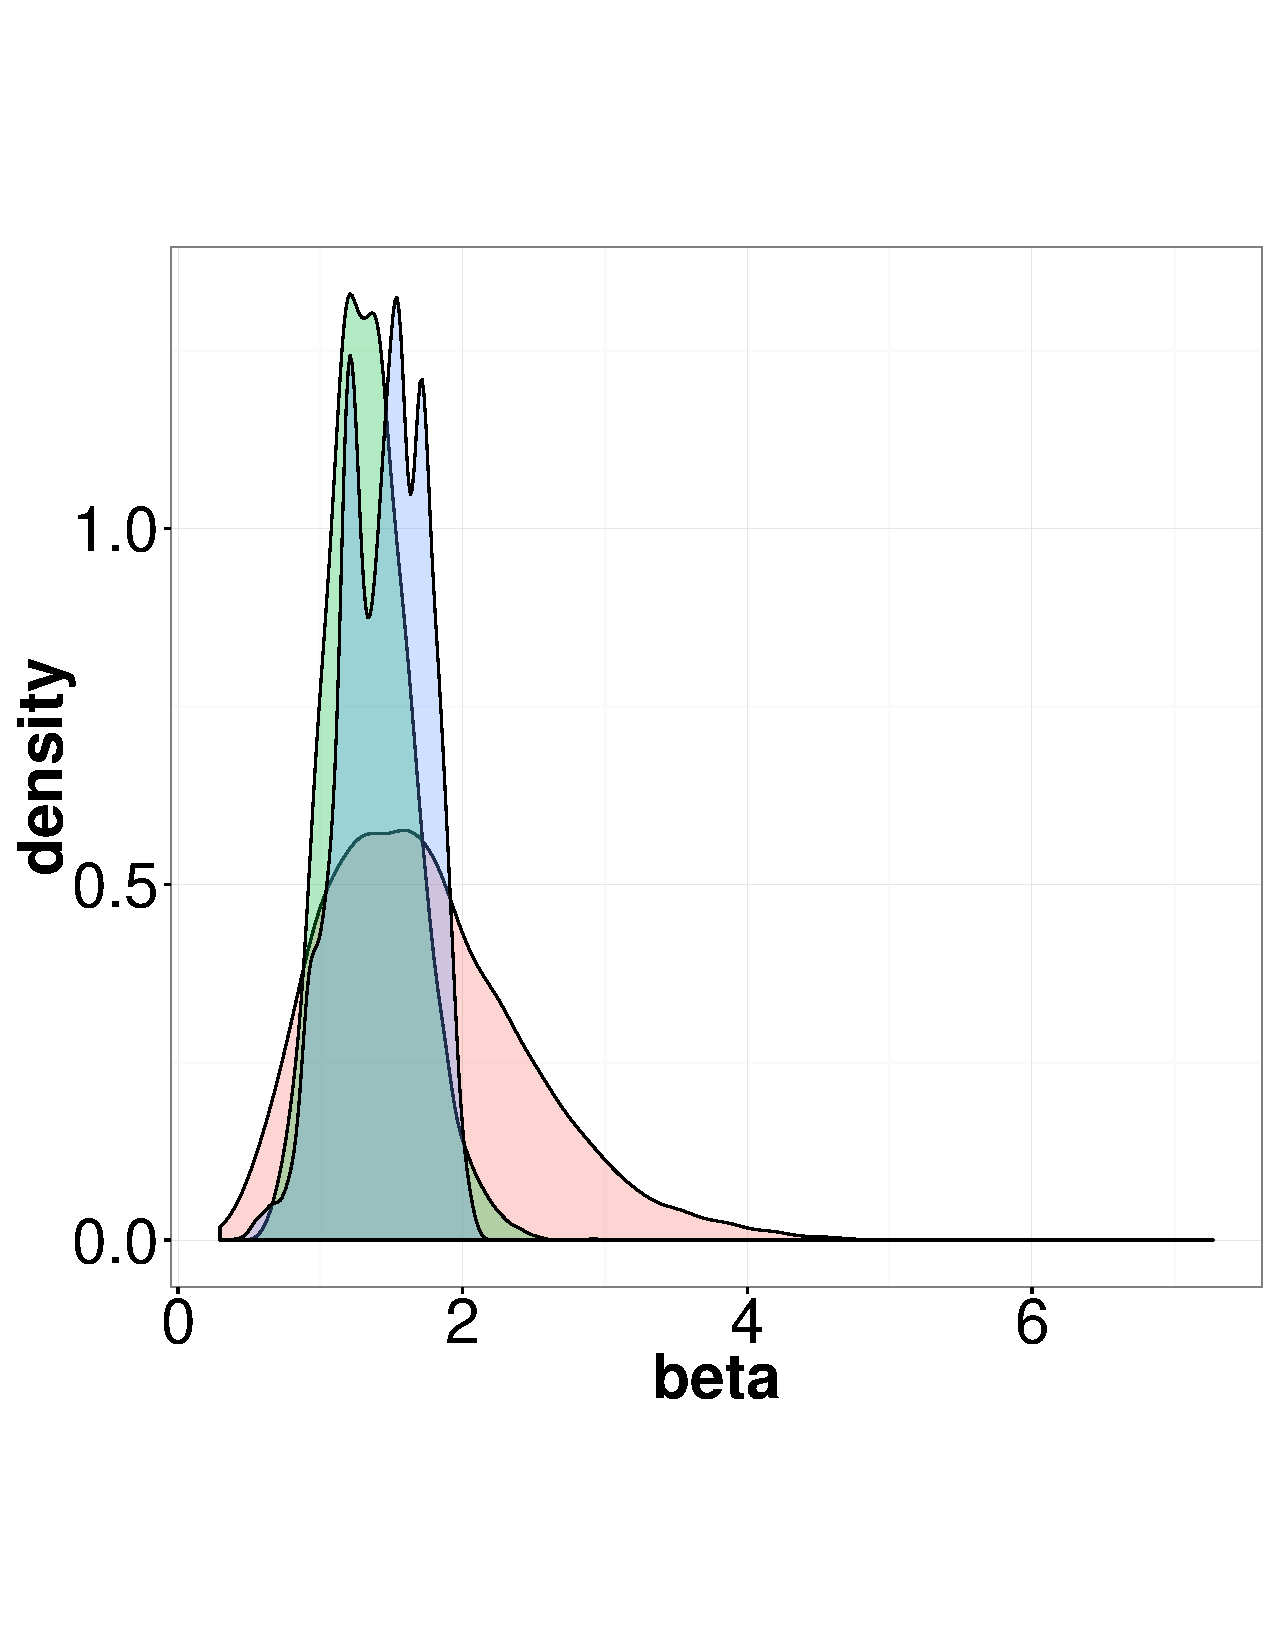
\includegraphics [width=0.98\textwidth, angle=0]{figs/dist_beta.pdf}
%   \vspace{0.2 in}
  \end{minipage}
% \begin{minipage}[!hp]{0.4\linewidth}
% \centering
%   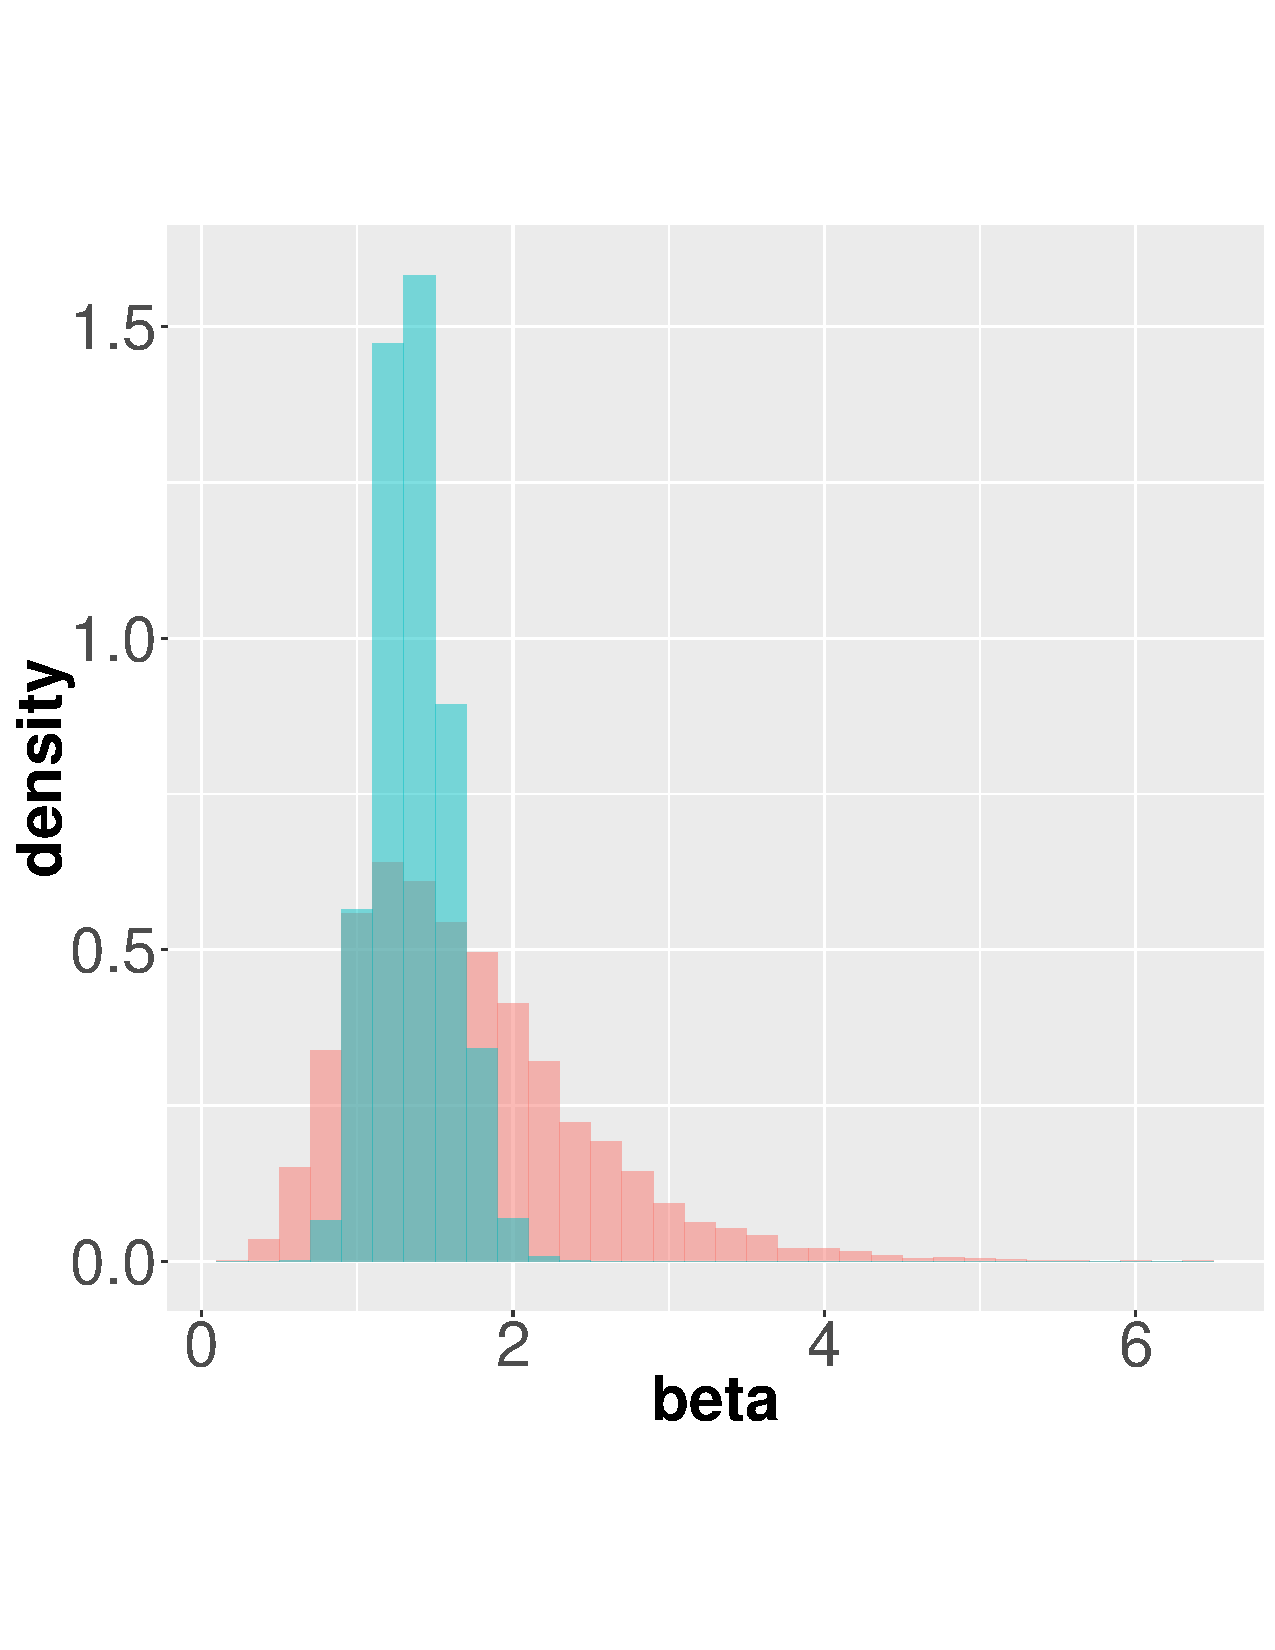
\includegraphics [width=0.90\textwidth, angle=0]{figs/hist_beta.pdf}
%   \vspace{-0 in}
% \end{minipage}
  \begin{minipage}[hp]{0.64\linewidth}
%   \vspace{-0.3 in}
  \caption{Prior distribution of an MJP parameter (the wide red density), with two conditional distributions. 
    Narrow dotted-green is the density conditioned on both the observations as well as a simulated MJP posterior. 
    The wider dashed-blue curve is density of interest: the marginal distribution of the parameters conditioned on observations. 
  Plots were produced from the experiment in section~\ref{sec:immig}.}
     \label{fig:hist}
  \end{minipage}
%   \vspace{-0.6 in}
  \end{figure}
  However, the Gibbs sampling approach coupling between path and parameters can result in a very sluggish exploration of parameter and path space. 
  We illustrate this in figure~\ref{fig:hist}~\citep[inspired by][]{papaspiliopoulos2007general}), which shows the posterior distribution of an MJP parameter (in dashed-blue) is less concentrated than the distribution conditioned on both observations as well the MJP trajectory (dotted-green). 
The coupling is strengthened as the trajectory grows longer, and the Gibbs sampler can mix very poorly for situations with long observation periods, even if the observations themselves are sparse and only mildly informative about the parameters.

% \subsection{A marginal sampler for MJP parameters} 
% For the discrete-time case, this problem of parameter-trajectory
% coupling can be circumvented by marginalizing out the MJP trajectory 
% and directly sampling from the posterior over parameters $P(\theta|X)$.
% In its simplest form (Algorithm~\ref{alg:disc_time_mh}), this 
% involves a Metropolis-Hastings scheme that proposes a new parameter 
% $\vartheta$ from some proposal distribution 
% $q(\vartheta|\theta)$, accepting or rejecting according to the usual
% Metropolis-Hastings probability. The latter step requires calculating the 
% marginal probabilities $P(X|\theta)$ and $P(X|\theta')$, integrating out
% the exponential number of possible latent trajectories. Fortunately,
% this marginal probability is a by-product of the forward-backward
% algorithm used to sample a new trajectory, so that no 
% additional computational burden is involved. 
% %The overall algorithm then is:
% \begin{algorithm}[H]
%   \caption{Metropolis-Hastings parameter inference for a discrete-time 
% Markov chain}
%    \label{alg:disc_time_mh}
%   \begin{tabular}{l l}
%    \textbf{Input:  } & \text{Observations $X$},
%    proposal density $q(\vartheta|\ctheta)$, and 
%    \text{previous parameters $\ctheta$}.\\
%    \textbf{Output:  }& \text{A new Markov chain parameter $\ntheta$}.\\
%    \hline
%    \end{tabular}
%    \begin{algorithmic}[1]
%   \State Propose a new parameter $\vartheta$ from the proposal distribution
%   $q(\vartheta|\ctheta)$.
%   \State Run the forward pass of the forward-backward algorithm to 
%     obtain the marginal likelihood of the observations, $P(X|\vartheta)$.
%     \State Set $\ntheta = \vartheta$ with probability 
%     $\min(1,\frac{P(X,\vartheta)q(\ctheta|\vartheta)}{P(X,\ctheta)q(\vartheta|\ctheta)})$, else 
%     $\ntheta = \ctheta$.
%   \State Sample a new path with
%     the backward pass of the forward-backward algorithm.
%     %for the chosen parameter.
% \end{algorithmic}
% \end{algorithm}

% %\vspace{-.35in}
% Constructing a marginal sampler over the MJP parameters by
% integrating out the continuous-time trajectory is harder.
% %the set of transition times is unbounded, with individual elements
% %unconstrained over the observation interval $[0,\cT]$.
% %Naively calculating this marginal probability for the continuous-time
% %case is not straightforward, as there is no finite set of candidate
% %times to make a pass over. 
% One approach~\citep{FearnSher2006} makes a sequential 
% forward pass through all {\em observations} $X$, using matrix exponentiation
% to marginalize out all
% continuous-time paths between successive times. As
% shown in~\cite{RaoTeh13}, this approach is cubic rather than 
% quadratic in the 
% number of states, cannot exploit structure like sparsity in the 
% transition matrix, and can depend in not trivial ways on the exact 
% nature of the observation process.
% Also, the number of expensive matrix exponentiations depends on
% the number of observations rather than the number of transitions.
% %
% %
% A second approach, particle MCMC~\citep{Andrieu10}, uses 
% particle filtering to get an unbiased estimate of the marginal 
% $P(X|\theta)$. Plugging this into the Metropolis-Hastings 
% acceptance probability results in an MCMC sampler that targets the 
% correct posterior, however %~\cite{Andrieu09}, 
% the resulting scheme does not exploit the structure 
% of the MJP, and we show that it is quite inefficient.

% The advantage of introducing the thinned events $U$ was demonstrated in 
% \cite{RaoTeh13, RaoTeh12} : this allows exploiting discrete-time 
% algorithms like FFBS for path sampling.
% %be brought to playthe thinning-based approach over matrix exponential and particle-MCMC
% %approaches for trajectory inference. 
% In the next section, we outline a \naive\  first attempt at extending this 
% approach to 
% parameter inference.
% We describe why this approach is not adequate, and then describe our
% final algorithm. % in the section after. 

\vspace{-.2in}
\section{\Naive\ parameter inference via Metropolis-Hastings}
%A natural approach to reduce the coupling in the Gibbs sampler is to reduce ?Bayesian fraction of missing information?. 
For discrete-time HMMs, path-parameter coupling can be circumvented by marginalizing out the Markov trajectory, and directly sampling from the marginal posterior $P(\theta|X)$.
In its simplest form, this involves a Metropolis-Hastings (MH) scheme that proposes a new parameter $\vartheta$ from some proposal distribution $q(\vartheta|\theta)$, accepting or rejecting according to the usual MH probability.
The marginal probabilities over $X$ given parameters are computed using the FFBS algorithm.
The Rao-Teh algorithm, which recasts posterior simulation for continuous-time models as discrete-time simulation on a random grid, then provides a simple mechanism to incorporate such an MH-scheme into continuous-time settings: directly update $\theta$, conditioning on the random grid $W$, but marginalizing out the states $(v_0, V)$.
%, following the scheme from Algorithm~\ref{alg:disc_time_mh}.
%The resulting scheme updates $\theta$ conditioned on the random 
%grid, but with the trajectory integrated out 

Specifically, given $\theta$ and the Poisson grid $W$, rather than simulating new path values (the backward pass in algorithm~\ref{alg:Unif_gibbs}), and then conditionally updating $\theta$ (the second step in algorithm~\ref{alg:MJP_gibbs}), we {\em first} propose a parameter $\vartheta$ from $q(\vartheta|\theta)$. This is accepted with probability 
$$ \texttt{acc} = \min\left(1, 
\frac{P(X|W,\vartheta) P(W|\vartheta)P(\vartheta)q(\theta|\vartheta)} {P(X|W,\theta) P(W|\theta)P(\theta)q(\vartheta|\theta)}\right),$$ 
%Only after accepting or rejecting do we simulate state values via a backward pass.
thereby targeting the distribution $P(W,\theta|X)$.
In the equation above, $P(X|W,\theta)$ is the probability of the observations $X$ given $W$ with $(v_0,V)$ marginalized out. 
Uniformization says this is the marginal probability of $X$ under a discrete-time HMM on $W$, with transition matrix $B(\theta)$. This can be computed using the forward pass of FFBS algorithm (steps 4 and 6 of algorithm~\ref{alg:MH_naive}). 
The term $P(W|\theta)$ is the probability of $W$ under a rate-$\Omega(\theta)$ Poisson process. 
These, and the corresponding terms for $\vartheta$ allow the acceptance probability to be computed.
%make a forward pass over $W$, and calculate and $P(X|W,\vartheta)$. % as in algorithm~\ref{alg:disc_time_mh}.
Only {\em after} accepting or rejecting $\vartheta$ do we simulate new states $(v'_0,V')$, using the new parameter $\theta'$ in a backward pass over $W$. 
%Then discard all self-transitions, resample $W$ and repeat. 
The new trajectory and parameter are used to simulate a new grid $W'$, and the process is repeated.
Algorithm~\ref{alg:MH_naive} includes all the details of this algorithm, with figure~\ref{fig:naive_mh} in the appendix sketching out the main idea.

%\vspace{-.1in}
%\vspace{-.32in}
\begin{algorithm}[H]
   \caption{\Naive\  MH for parameter inference for MJPs }
   \label{alg:MH_naive}
  \begin{tabular}{l l}
   \textbf{Input:  } & \text{Observations $X$}, 
                       \text{the MJP path $S(t) = (s_0, S, T)$, the  parameters $\theta$ }and $\pi_0$.\\ 
      %               & \text{A  Metropolis-Hasting proposal $q(\cdot | \theta)$}.\\
   \textbf{Output:  }& \text{A new MJP trajectory $S'(t) = (s'_0, S', T')$, 
                            new MJP parameters $\theta'$}.\\
   \hline
   \end{tabular}
   \begin{algorithmic}[1]
     \State Set $\Omega(\theta) > \max_s{A_s(\theta)}$ for
     some function $\Omega(\cdot)$, e.g.\ $\Omega(\theta) = 
      2\max_s A_s(\theta)$.
      \State \textbf{Simulate the thinned times $U$} from a rate-$(\Omega(\theta)-A_{S(t)}(\theta))$ Poisson process: 

      $\qquad \qquad \qquad \qquad U \sim \text{PoissProc}(\Omega(\theta) - A_{S(t)}(\theta)).$

      \State 
      Set $W = T \cup U$ and discard $(s_0,S)$. Define $\tilde{W} = 0 \cup W \cup t_{end}$.
    \State 
    \textbf{Forward pass:}
    Set $B(\theta) = I + \frac{1}{\Omega(\theta)}A(\theta)$ and
    $\fwd^\theta_0(\cdot) = \pi_0$.
 %   Sequentially update $\fwd^\theta_i(\cdot)$ at time $w_i \in W$ as: 
\vspace{-.1in}
    $$\textbf{for } i=1\rightarrow |\tilde{W}|\textbf{ do:} \quad \fwd^{\theta}_i(s') = \sum_{s \in \cS} \ell_{i-1}(s) \cdot \fwd^\theta_{i-1}(s)\cdot B_{ss'}(\theta), \quad \forall s' \in \cS.\qquad\qquad\quad $$
    \State \textbf{Propose $\vartheta \sim q(\cdot| \theta)$.}
    For all elements of $\tilde{W}$, calculate $\fwd^\vartheta_i(\cdot)$ similar to above.
      \State \textbf{Accept/reject:} 
      Set $P(X|W,\theta) = \sum_{s \in \cS} \fwd_{|\tilde{W}|}^\theta(s),$ $P(W|\theta) = \Omega(\theta)^{|W|}\exp(-\Omega(\theta)t_{end})$, with similar expressions for $\vartheta$. 
      With probability $\texttt{acc}$, set $\theta'$ to $\vartheta$, else set it to $\theta$, where: %Here 
      %The acceptance probability for $\vartheta$ is given by 
%         \vspace{-.05in}
          \begin{align}
            \label{eq:ncp_acc}
            \texttt{acc} &=  1 \wedge \frac{P(\vartheta|W, X)}{P(\theta|W, X)} \frac{q(\theta|\vartheta)}{q(\vartheta|\theta)}
          =  1 \wedge \frac{P(X| W,\vartheta) P(W | \vartheta)P(\vartheta)}
            {P(X|W, \theta)P(W | \theta)P(\theta)} \frac{q(\theta|\vartheta)}{q(\vartheta|\theta)}.
          \end{align}
%         \vspace{-.1in}
          %$P(X|W,\vartheta) = \sum_{s \in \cS} \fwd_{|W|}^\vartheta(s) $. Use these, and the fact that $P(W|\theta)$ is Poisson-distributed to accept or reject the proposed $\vartheta$. Write the new parameter as $\theta'$.
    %as \boqian{$(W,\theta,\vartheta)$}.
    \State %For the new parameter $\theta'$, simulate states $V$. 
    \textbf{Backward pass:}
    Set $v_{|W|} \sim \bck^{\theta'}_{|W|}(\cdot)$, where $\bck^{\theta'}_{|W|}(s) \propto \fwd^{\theta'}_{|W|}(s)\cdot\ell_{|W|}(s) \quad \forall s \in \cS.$ 
    %at time $w_i$ given $v_{i+1}$  at time $w_{i+1}$:
\vspace{-.1in}
    $$ \textbf{for } i=(|W|-1)\rightarrow 0\textbf{ do:} \quad v_i \sim \bck^{\theta'}_i(\cdot),\ \ \text{where } 
    \bck^{\theta'}_i(s) \propto \fwd^{\theta'}_i(s)\cdot B_{sv_{i+1}}(\theta') \cdot \ell_i(s)  \ \forall s \in \cS.$$
   % Here, $\bck^{\theta'}_{|W|}(\cdot) = \fwd^{\theta'}_{|W|}(\cdot)$.  This completes the FFBS algorithm.
    \State Set $s'_0=v_0$. Let $T'$ be the set of times in $W$ when $V$ changes state. Define $S'$ as the corresponding set of state values. Return $(s'_0, S', T', \theta')$.
\end{algorithmic}
\end{algorithm}
\vspace{-.1in}
The resulting MCMC algorithm updates $\theta$ with the MJP trajectory 
integrated out, and by instantiating less `missing' information, can be expected to mix better. 
This can be quantified by the so-called Bayesian fraction of missing information~\citep{liu1994fraction, papaspiliopoulos2007general}. 
The Gibbs sampler of algorithm~\ref{alg:MJP_gibbs} can be viewed as operating on a centered parametrization~\citep{papaspiliopoulos2007general} or sufficient augmentation~\citep{yu2011center} of a hierarchical model involving $\theta$, the Poisson events $W$, and the state values $(v_0,V)$. The MH algorithm reverses the order in which the path and parameter are updated, and is closely related to noncentered parametrizations or ancillary augmentations. 
For a detailed review of the suitability of these two approaches, as well as ways to combine them together, we refer to~\citet{papaspiliopoulos2007general, yu2011center}.

We note that even with the state values $(v_0,V)$ marginalized out, $\theta$ is updated {\em conditioned on $W$}. 
The distribution of $W$ depends on $\theta$: $W$ follows a rate-$\Omega(\theta)$ Poisson process. This dependence manifests in the $P(W|\theta)$ and $P(W|\vartheta)$ terms in equation~\eqref{eq:ncp_acc}. 
The fact that the MH-acceptance involves the probability of the observations  $X$ is inevitable, however the $P(W|\theta)$ term is an artifact of the computational algorithm of Rao-Teh. 
In our experiments, we show that this term significantly affects acceptance probabilities and mixing. 
For parameter $\theta$, $|W|$ is Poisson distributed with mean and variance $\Omega(\theta)$. 
If the proposed $\vartheta$ is such that $\Omega(\vartheta)$ is half $\Omega(\theta)$, then the ratio $P(W|\vartheta)/P(W|\theta)$ will be small, and $\vartheta$ is unlikely to be accepted. 
%, resulting in a low acceptance probability.  
This will slow down mixing.
The next section describes our main algorithm that gets around this.


\section{An improved Metropolis-Hasting algorithm}
\vspace{-.05in}
Our main idea is to symmetrize the probability of $W$ under the old and 
proposed parameters, so that 
$P(W|\theta)$ disappears from the acceptance ratio. This results
in a significantly more efficient, and also a simpler MCMC scheme.
%This forms the main contribution of this paper.
As before, the MCMC iteration begins with the pair $(S(t), \theta)$. 
Instead of simulating the Poisson events $U$, we first generate a new 
parameter $\vartheta$ from $q(\vartheta|\theta)$. Treat this as an 
auxiliary variable, so that the augmented space now is the triplet 
$(S(t), \theta,\vartheta)$. We pretend $S(t) \equiv (S,T)$ was sampled by  
uniformization, where the dominating Poisson rate $\Omega$ equals 
$(\Omega(\theta) + \Omega(\vartheta))$ instead of just $\Omega(\theta)$ 
(recall any choice greater than $\max_s A_s$ is valid).
Now the set of thinned events $U$ is piecewise-constant
Poisson with intensity $\Omega(\theta) + \Omega(\vartheta) - 
A_{S(t)}$. Following algorithm~\ref{alg:Unif_gibbs} or~\cite{RaoTeh13}, 
the {\em a priori} probability of the reconstructed set $W = U \cup T$, 
$P(W|\theta,\vartheta)$, is a homogeneous Poisson 
%the union of $U$ with the actual trajectory transition times $T$, 
process with rate $\Omega(\theta) + \Omega(\vartheta)$. Discard all 
MJP state information, so that the MCMC state space is $(W, \theta, \vartheta)$,
and propose swapping $\theta$ with $\vartheta$. 
Observe from
symmetry that the Poisson skeleton $W$ has the same probability both
before and after this proposal, so that unlike the previous scheme,
the ratio $P(W|\vartheta)/P(W|\theta)$ equals $1$.  This simplifies 
computation, and significantly improves mixing.
The acceptance probability 
%depends only on the probability of the observations
%under both set of parameters, %as we can use the forward-backward algorithm
%to calculate this. Our acceptance probability 
equals
$ 
  \min\left(1, \frac{P(X,\vartheta)q(\theta|\vartheta)}
   {P(X,\theta)q(\vartheta|\theta)}\right) = 
  \min\left(1, \frac{P(X|\vartheta)p(\vartheta)q(\theta|\vartheta)}
   {P(X|\theta)p(\theta)q(\vartheta|\theta)}\right).
   $
   The terms $P(X|\vartheta)$ and  $P(X|\theta)$ can be calculated by 
   running a forward pass of the forward-backward algorithm, and after
   accepting or rejecting the proposal, a new trajectory is sampled by
   completing the backward pass. Finally, the thinned events are
   discarded. We sketch out our algorithm in Algorithm~\ref{alg:MH_improved}
   and figure~\ref{fig:MH_improved} in the appendix. 
\begin{algorithm}[H]
   \caption{Symmetrized MH for parameter inference for MJPs }
   \label{alg:MH_improved}
  \begin{tabular}{l l}
   \textbf{Input:  } & \text{The observations $X$,}
                      \text{the MJP path $S(t) = (S, T)$, parameters $\theta$} and $\pi_0$.\\ 
                     & \text{A  Metropolis-Hasting proposal $q(\cdot | \theta)$}.\\
   \textbf{Output:  }& \text{A new MJP trajectory $S'(t) = (S', T')$, 
                            new MJP parameters $\theta'$}.\\
   \hline
   \end{tabular}
   \begin{algorithmic}[1]
      \State Sample $\vartheta \sim q(\cdot| \theta)$, and 
      set %$\Omega = \max_i A_i(\theta) + \max_i A_i(\theta^*)$. 
	$\Omega \assign \Omega(\theta) + \Omega(\vartheta)$ for some function 
    $\Omega(\theta) \ge \max_s A_s(\theta)$.
      %In the case of uniformization, we
      %have a single $\Omega$ for all states, with $\Omega = \max_i A_i(\theta) + \max_i A_i(\theta^*)$.
      %, with $h(\theta) > max_s{|A_s(\theta)|}$, $h(\theta^*) > max_s{|A_s(\theta^*)|}$ using some deterministic function $h$.
    \State Sample thinned jumps $U\subset[0, t_{end}]$ from a Poisson process with 
    piecewise-constant rate $R(t) = (\Omega - A_{S(t)}(\theta))$. 
    Set $W = T \cup U$ and discard MJP states.
    \State The current MCMC state-space is $(W,\theta,\vartheta)$. Propose swapping
    $\theta$ and $\vartheta$. %the new state-space is 
   %\boqian{ $(W, \vartheta, \theta)$.}
%$(W, \theta, \vartheta)$    
     The acceptance probability is given by
   % accept $\theta^*$ as $\tilde{\theta}$ with probability $\alpha$.
     \vspace{-.15in}
        \begin{align*}
        \alpha %&=  1 \wedge \frac{P(W,(\vartheta, \theta)| y)}{P(W, (\theta, \vartheta)| y)}\\
       % &=  1 \wedge \frac{P(y| W,\vartheta, \theta) P(W | (\vartheta, \theta))p((\vartheta, \theta))}{P(y| W,(\theta, \vartheta)) P(W | (\theta, \vartheta))p((\theta, \vartheta))}\\
        &=  1 \wedge \frac{P(X| W,\vartheta,\theta)p(\vartheta)q(\theta|\vartheta)}
        {P(X| W,\theta, \vartheta)p(\theta) q(\vartheta|\theta)}.
        \end{align*}
    \State For both $\theta$ and $\vartheta$, make a forward pass through the 
    elements of $W$, sequentially updating the distribution over states at 
    $w \in W$ given observations up to $w$. At the end, we have calculated
    $P(X|W,\theta, \vartheta)$ and $P(X|W,\vartheta, \theta)$. Use these to accept or reject the
    proposed swapping of $\theta$ and $\vartheta$. Write the new state-space
    as $(W,\theta',\vartheta')$.
    \State For the new transition matrix $B(\theta',\vartheta')$, make a backward pass through 
    the elements of
    $W$, sequentially assigning a state to each element $w_i \in W$ given 
    $w_{i+1}$.
%    Sample a path $\tilde{V}$, from a discret-time Markov chain with $|W| + 1$ steps, using FFBS algorithm. The transition matrix of the Markov chain is $B = (I + \frac{A(\tilde{\theta})}{\Omega})$ while the initial distribution over states is $\pi_0$. The likelihood of state $s$ at step $i$ is 
%    $$ L_i(s) = P(Y_{[w_i, w_{i + 1})} | S(t) = s \; for\; t \in [w_i, w_{i + 1})) = \prod_{j: t_j \in [w_i, w_{i + 1})}p(y_{t_j} | S(t_j) = s).$$\\
%%(i.e. $V(i) \sim P(V |  \theta(i), W(i - 1), y).$) Then delete all the virtual jumps to get $S(i), T(i) .$\\
    \State Let $T'$ be the set of times in $W$ when the Markov chain changes state. Define $S'$ as the corresponding set of state values. Return $(S', T', \theta')$.
\end{algorithmic}
\end{algorithm}


%\subsection{Correctness of the proposed algorithm }
%\label{sec:verify2}
\begin{proposition}
  The sampler described in Algorithm~\ref{alg:MH_improved} has the posterior
  distribution $p(\theta,S(t)|X)$ as its stationary distribution.
\end{proposition}
\begin{proof}
  Suppose that at the start of the algorithm, we have a pair $(\theta,S(t))$ from
  the posterior distribution $p(\theta,S(t)|X)$. Introducing $\theta^*$
  from $q(\theta^*|\theta)$ results in a triplet whose marginal over the first
  two variables is still $p(\theta,S(t)|X)$.

  Sampling $U$ from a Poisson process with rate $\Omega(\theta) +
  \Omega(\theta^*) - A_{S(t)}(\theta)$, results in a random grid $W = T \cup U$
  that is distributed according to a rate $\Omega(\theta) + \Omega(\theta^*)$
  Poisson process (Proposition 2 in~\cite{RaoTeh13}). Discarding all state 
  information results in a triplet $(W,\theta,\theta^*)$ with probability
  proportional to $p(\theta)q(\theta^*|\theta)p(W|\theta,\theta^*)
  p(X|W,\theta,\theta^*)$.

Next we propose swapping $\theta$ and $\theta^*$, since this
is a deterministic proposal, the MH-acceptance probability is given by
$$\alpha = 1 \wedge \frac{p(\theta^*)q(\theta|\theta^*)p(W|\theta^*,\theta)
p(X|W,\theta^*,\theta)}{p(\theta)q(\theta^*|\theta)p(W|\theta,\theta^*)
p(X|W,\theta,\theta^*)}$$
The term $p(W|\theta,\theta^*)$ is just a Poisson process with rate $\Omega(\theta)+
\Omega(\theta^*)$, so that $p(W|\theta,\theta^*) = p(W|\theta,\theta^*)$. The
two terms $p(X|W,\theta,\theta^*)$ and $p(X|W,\theta^*,\theta)$ are obtained
at the end of a forward pass over $W$ using discrete-time transition matrices
$B(\theta,\theta^*) = \left(I + \frac{A(\theta)}{\Omega(\theta)+\Omega(\theta^*)}\right)$ 
and $B(\theta^*,\theta) = \left(I + \frac{A(\theta^*)}{\Omega(\theta)+\Omega(\theta^*)}\right)$. 

Calling the parameters 
after the accept step $(\tilde{\theta}, \tilde{\theta}^*)$, we have that
$(\tilde{\theta}, \tilde{\theta}^*,W)$ has the same distribution as
$(\theta, \theta^*,W)$.
Finally, following Lemma 1 in~\cite{RaoTeh13}, using the matrix 
$B(\tilde{\theta},\tilde{\theta}^*)$ to make a backward pass through $W$,
and discarding the self-transitions results in a trajectory $(\tilde{S}(t)$
distributed according to $A(\tilde{\theta})$. Discarding the auxiliary parameter
$\tilde{\theta}^*$ results is a pair $(\tilde{\theta},\tilde{S}(t))$ from
the posterior.
% \begin{align*}
%  p(y, W, S, T, \theta, \theta^*) &= p(\theta) q(\theta^* | \theta) P(S,T| \theta, \theta^*) P(W| S, T, \theta, \theta^*)P(y | S, T, \theta, \theta^*)\\
%  &=p(\theta) q(\theta^* | \theta) P(S,T| \theta) P(W| S, T, \theta, \theta^*)P(y | S, T).
% \end{align*}
% The marginal distribution of $(y, S, T, \theta, \theta^*)$ and $(y, S, T, \theta)$ as follows.\\
% \begin{align*}
%  p(y, S, T, \theta, \theta^*) &= p(\theta) q(\theta^* | \theta) P(S,T| \theta, \theta^*)P(y | S, T, \theta, \theta^*)\\
%  &=P(y, S, T, \theta) q(\theta^* | \theta).
% \end{align*}
% \begin{align*}
%  p(y, S, T, \theta) &= p(\theta)P(S,T| \theta)P(y | S, T, \theta).
% \end{align*}
% So the conditional distribution over $\theta^*$ given $(y, S, T, \theta)$ is $q(\theta^* | \theta)$. And the conditional distribution over W given $(y, S, T, \theta, \theta^*)$  is $P(W | S, T, \theta, \theta^*)$, which is actually the distribution of Non Homogeneous Poisson Process with piecewise constant rate $h(\theta) + h(\theta^*) - A_{S(t)}(\theta)$.\\
% Thus the Step 1 + Step 2 is actually equivalent to sampling from the conditional distribution $P(\theta^* , W| S, T, \theta, y)$.\\
% The Step 3 + Step 4 satisfy the detailed balance condition. The reason is as follows.
% \begin{align*}
% &P((W, S, T, (\theta, \theta^*)) \rightarrow (W, S^*, T^*, (\theta^*, \theta))) P(S,T, (\theta, \theta^*) | W, y)\\
% &= (1 \wedge \frac{P((\theta^*,\theta) | W, y)}{P((\theta,\theta^*) | W, y)})P(S^*, T^* | W, (\theta^*, \theta), y)P(S, T | W, (\theta, \theta^*), y)P((\theta, \theta^*) | W, y)\\
% &= P((W, S^*, T^*, (\theta^*, \theta)) \rightarrow (W, S, T, (\theta, \theta^*))) P(S^*,T^*, (\theta^*, \theta) | W, y)
% \end{align*} 
% Therefore the stationary distribution of this MCMC sampler is $P(W, S, T, (\theta, \theta^*) | y)$. Thus the stationary distribution of $(S, T, \theta)$ is the corresponding marginal distribution $P(S, T, \theta | y)$.  
\end{proof}





\section{Experiments}\label{sec:expts}~
In the following, we evaluate Python implementations of our two proposed
algorithms, the \naive\ MH algorithm (algorithm~\ref{alg:MH_naive}, which we
plot in yellow) and its symmetrized improvement (algorithm~\ref{alg:MH_improved}, 
which we call symmetrized MH and plot in red). We compare different variants of 
these algorithms, corresponding to different uniformizing Poisson rates 
(i.e.\ different choices of $\kappa$, see section~\ref{sec:comments}). For 
\naive\ MH, %~\ref{alg:MH_naive}, 
we set $\Omega(\theta) = \kappa \max_s A_s(\theta) $ with $\kappa$  equal to 
$1.5, 2$ and $3$, represented in our plots with circles, triangles and square
symbols. For symmetrized MH, %algorithm~\ref{alg:MH_improved}, 
where the uniformizing rate depends 
on both the current and proposed parameter, we consider two settings
 $\Omega(\theta, \vartheta) = \kappa (\max A(\theta) + \max A(\vartheta))$ 
 ($\kappa = 1$ and $1.5$, plotted with {triangles} and {squares}), and 
$\Omega(\theta, \vartheta) = \kappa \max(\max A(\theta), \max A(\vartheta))$
($\kappa=1.5$, plotted with {circles}).  We compare these
algorithms against two baselines: Gibbs sampling (algorithm~\ref{alg:MJP_gibbs},
plotted in blue), and particle MCMC~\cite{Andrieu10}, plotted in black. Gibbs
sampling involves a uniformization step to update the MJP trajectory, and for this
we used three settings, $\kappa=1.5,2,3$, plotted with circles, {triangles}
and {squares}.  Unless specified, our results were
obtained from $100$ independent MCMC runs, each consisting of $10000$ iterations.
We found particle MCMC to be more computationally intensive, and limited each 
run to $3000$ iterations, the number of particles being $5, 10$ and $20$ 
(plotted with circles, trianges and squares). 

% We also considered exploiting gradient information of the target distribution to 
% apply Hamiltonian Monte Carlo (HMC)~\cite{Neal2010}. In particular, the forward 
% pass of FFBS allows us to also calculate the gradient of the log-probability with
% respect to the MJP parameters. We can exploit this information for more directed
% explorations of parameter space than a random-walk algorithm. Of course, this 
% comes at a higher computational cost. We evaluate HMC with the number of leapfrog
% steps taking values in $1, 3, 5$ or $10$, and the leapfrog stepsize taking values 
% in $0.02, 0.05$ and $0.1$. 

For each run of each MCMC algorithm, we calculated the effective sample size 
(ESS) of the posterior samples of the MJP parameters using the R package 
\texttt{rcoda}~\cite{Rcoda2006}. This estimates the number of independent 
samples returned by the MCMC algorithm, and dividing this by the runtime of a 
simulation gives the ESS per unit time. We used this measure to compare 
different samplers and different parameter settings.

% \begin{algorithm}[!ht]
%    \caption{Generic Gibbs sampling for MJPs for Gamma priors}
%    \label{alg:Generic Gibbs}
% \begin{algorithmic}
%    \State {\bfseries Input:} observations $y_{[t_0, t_{k+1})}$
%    \State Initialize, $i = 0$
%    \\ (a) Set $\alpha(0), \beta(0)$ arbitrarily and set current trajectory $[S,T](0)$ arbitrarily.\\
%     (b) Uniformize $[S,T](0)$, to get virtual jumps $U$.
%    \Repeat
%    \For{$i=1$ {\bfseries to} $N$}
%     \State (a) Sample $U(i) \sim P( U | \beta(i - 1), \alpha(i - 1), S(i - 1), T(i - 1), y)$.\\	
%     \State (b) Use FFBS algorithm to  sample states given all the jump times(both true jumps and virtual jumps).
% (i.e. $V(i) \sim P(V |  \beta(i - 1), \alpha(i - 1), W(i ), y).$) Then delete all the virtual jumps to get $S(i), T(i) .$\\
%     \State (c) Propose $\beta^* \sim q(.| \beta(i -1))$.\\
%       Set $\beta(i) = \beta^*$, with probability $P_{acc} = 1 \wedge \frac{P(\beta^* |S(i), T(i))}{P(\beta(i - 1) |S(i), T(i))} \frac{q(\beta(i - 1)|\beta^*)}{q(\beta^*|\beta(i - 1))}$;\\Otherwise set $\beta(i) = \beta(i-1)$.\\	  
%     \State (d) Sample $\alpha(i) \sim P(. | \beta(i), S(i), T(i), y)$.\\ It is a $Gamma(\mu + N, \lambda + \sum_{0}^NF_{S_i}(\beta)(t_{i + 1} - t_i))$ distribution actually.\\
%     \EndFor
%     \Until{$ i = N$ }
%  \end{algorithmic}
%  \end{algorithm}

\subsection{A simple synthetic MJP}
  \begin{figure}[H]
  \centering
  \begin{minipage}[!hp]{0.45\linewidth}
  \centering
    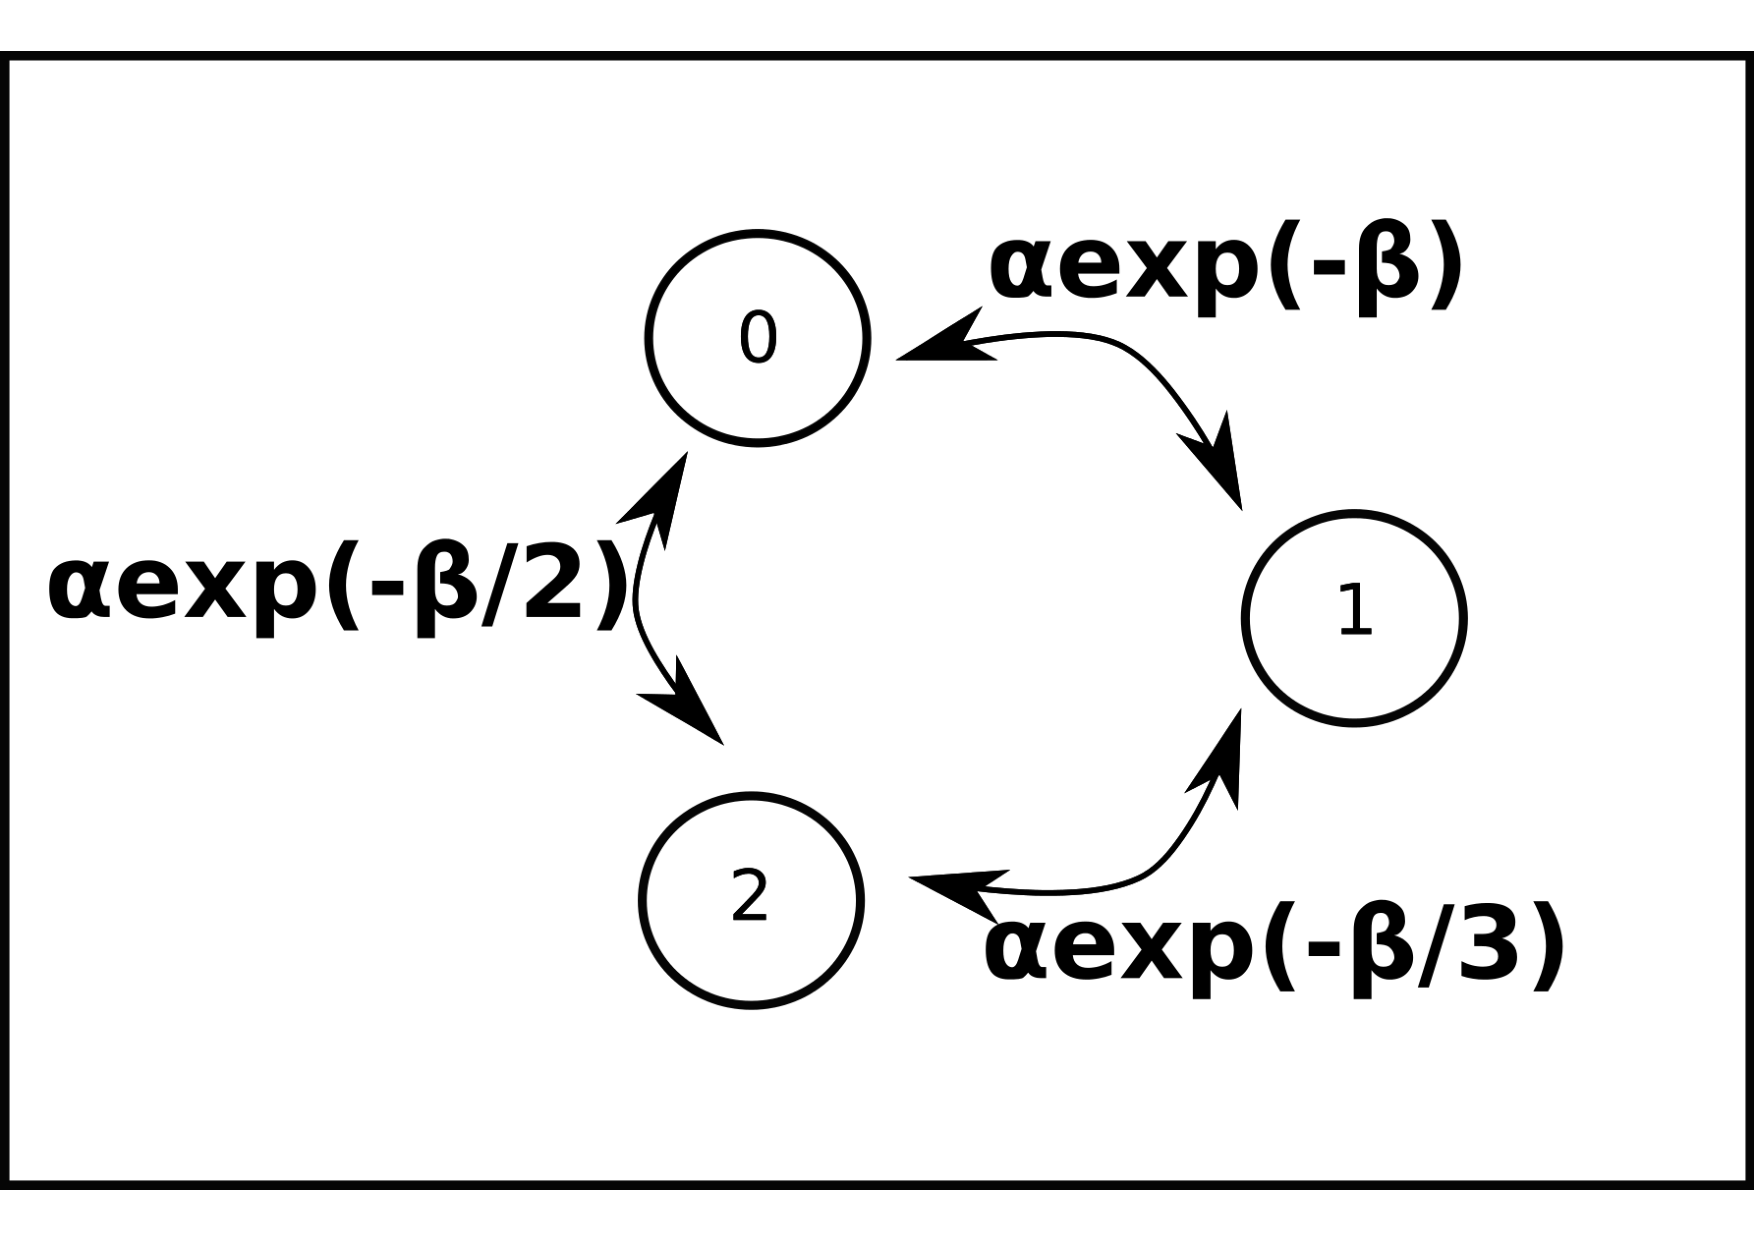
\includegraphics [width=0.70\textwidth, angle=0]{figs/exp_model.pdf}
      \end{minipage}
    \caption{A 3-state MJP with exponentially decaying rates}
    \label{fig:exp_model}
  \end{figure}

% \noindent Assume: $S = [S_0,S_1, ...,S_N] \;, T = [t_0(t_{start}), t_1,...,t_N, t_{N+1}(t_{end})]$, and y as observations.\\
% We consider a specific structure of rate matrix $A$. $A_{ij} = \alpha f_{ij}(\beta), \; i \neq j$. $A_{ii} = -\sum_{j \neq i} A_{ij}$. $0 \leq f_{ij} \leq 1$. Denote $F_i(\beta) = \sum_{j \neq i} f_{ij}(\beta)$.\\
% \begin{align*}
% P(s_0, S, T | \alpha, \beta) &= \pi_0(s_0)\prod_{i = 1}^N A_{S_{i - 1}S_i} \exp(- \int_{t_{start}}^{t_{end}} |A_{S(t)}| dt)\\
% &= \pi_0(s_0) \alpha^N \prod_{i = 1}^N f_{S_{i - 1}S_i} \exp(-\alpha  \sum_{i = 0}^{N} F_{S_i}(\beta)(t_{i + 1} - t_i))\\
% \end{align*} 
\noindent Consider an MJP with two parameters $\alpha$ and $\beta$, 
transitions between states $i$ and $j$ having rate $\alpha \exp(-\beta/(i+j))$.
We consider three settings: $3$ states (figure~\ref{fig:exp_model}),
$5$ states, and $10$ states.
We place Gamma$(\alpha_0,\alpha_1)$, and Gamma$(\beta_0, \beta_1)$ priors on 
the parameters $\alpha$ and $\beta$, with $(\alpha_0,\alpha_1,\beta_0,\beta_1)$ 
having values $(3,2,5,2)$ respectively. For each run, we draw random parameters 
from the prior to construct a transition matrix $A$, and placing a uniform 
distribution over states at time $0$, simulate an MJP trajectory.
We simulate observations uniformly at integer values on the time interval 
$[0, 20]$. Each observation is Gaussian distributed with mean equal to the state
at that time, and variance equal to $1$.  For the Metropolis-Hastings proposal, 
we used a lognormal distribution centered at the current parameter value, with 
a user-specified variance.
%\vinayak{We studied our MH sampler, for three setting of $k$}.  
% %\begin{align*}
% %P(\alpha, \beta | s_0, S, T ) \propto \alpha^N \prod_{i = 1}^N f_{S_{i - 1}S_i} \exp(-\alpha  \sum_{i = 0}^{N} F_{S_i}(\beta)(t_{i + 1} - t_i)) p_1(\alpha)p_2(\beta)\\
% %\end{align*}
% %If we assume the priors of $\alpha$, $\beta$ are $Gamma(\mu, \lambda)$, $Gamma(\omega, \theta)$, then the posterior will have a simper form as follows. 
% \begin{align*}
% P(\alpha, \beta | s_0, S, T ) = C \alpha^{\mu + N - 1}\exp(-\alpha (\lambda + \sum_{i = 0}^{N} F_{S_i}(\beta)(t_{i + 1} - t_i))) \prod_{i = 1}^N f_{S_{i - 1}S_i}  \beta ^{\omega - 1} \exp(-\theta \beta)\\
% \end{align*}
% We notice that given $\beta,\; S,\; T$, $\alpha$ is distributed as a $Gamma$ distribution.\\
% $\alpha | \beta, S, T, y  = \alpha | \beta, S, T \sim Gamma(\mu + N, \lambda + \sum_{0}^NF_{S_i}(\beta)(t_{i + 1} - t_i))$.\\
% There is no conjugate distribution to sample $\beta \sim P(\beta| s_0, S, T)$. We will have to use Metropolis Hasting within Gibbs to sample $\beta$. The target distribution is the following one.
% $$ P(\beta | S, T) = C \frac{\prod_{i = 1}^N f_{S_{i -1}S_i}(\beta)\beta^{\omega - 1} \exp(-\theta \beta)}{(\lambda + \sum_{i = 0}^{N} F_{S_i}(\beta)(t_{i + 1} - t_i))^{\mu + N}}.$$
% Such doubling might slow the mixing of the Markov chain. We can apply our Metropolis Hasting algorithm on this model.

\noindent \textbf{Results:}
  \begin{figure}%[b]
  \centering
  \begin{minipage}[!hp]{0.8\linewidth}
  \centering
    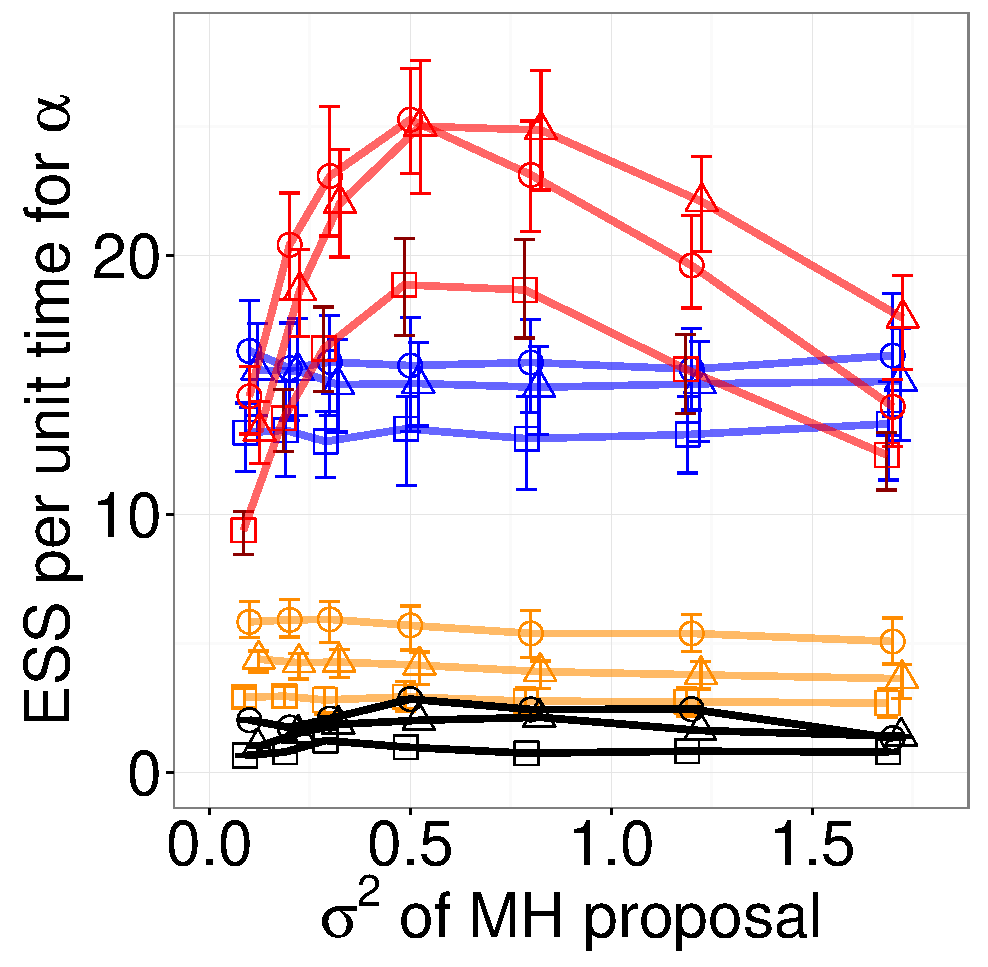
\includegraphics [width=0.45\textwidth, angle=0]{figures_new_apr12/exp_alpha_dim3_18apr12.pdf}
    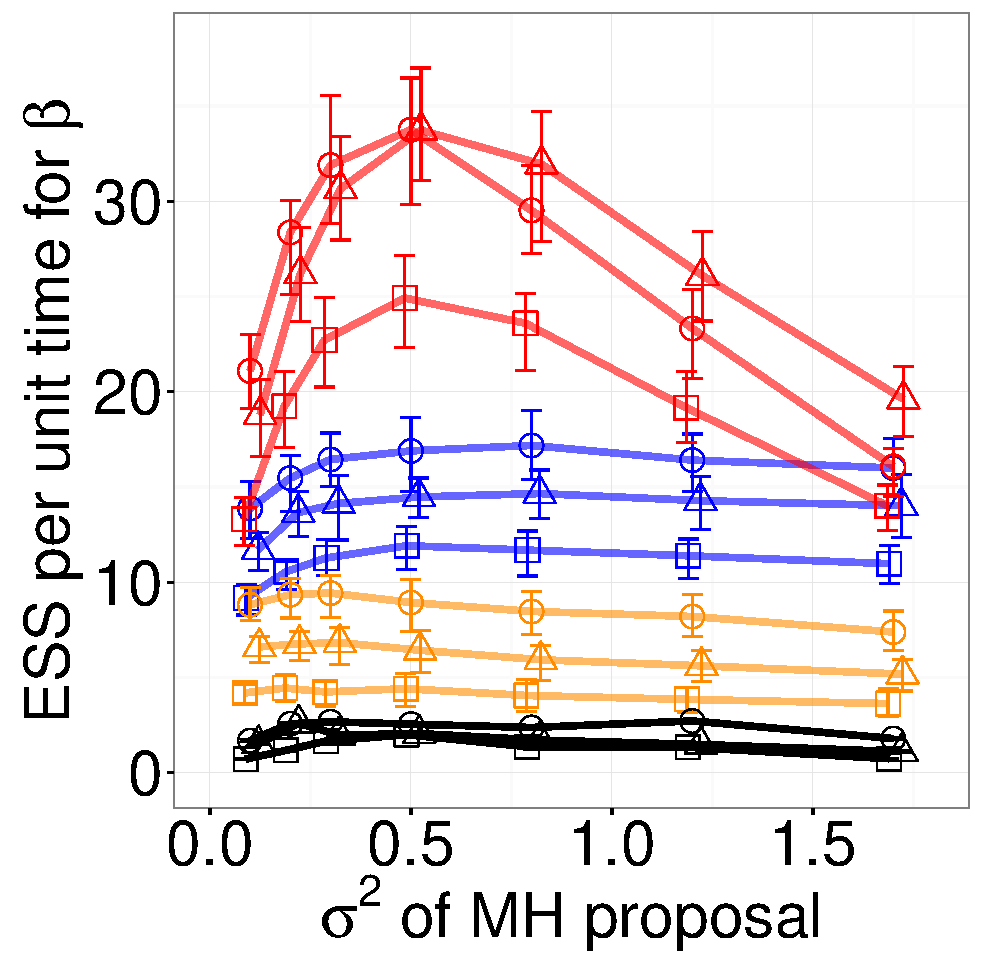
\includegraphics [width=0.45\textwidth, angle=0]{figures_new_apr12/exp_beta_dim3_18apr12.pdf}
%  \vspace{-1in}
  \end{minipage}
  \begin{minipage}[!hp]{0.8\linewidth}
  \centering
    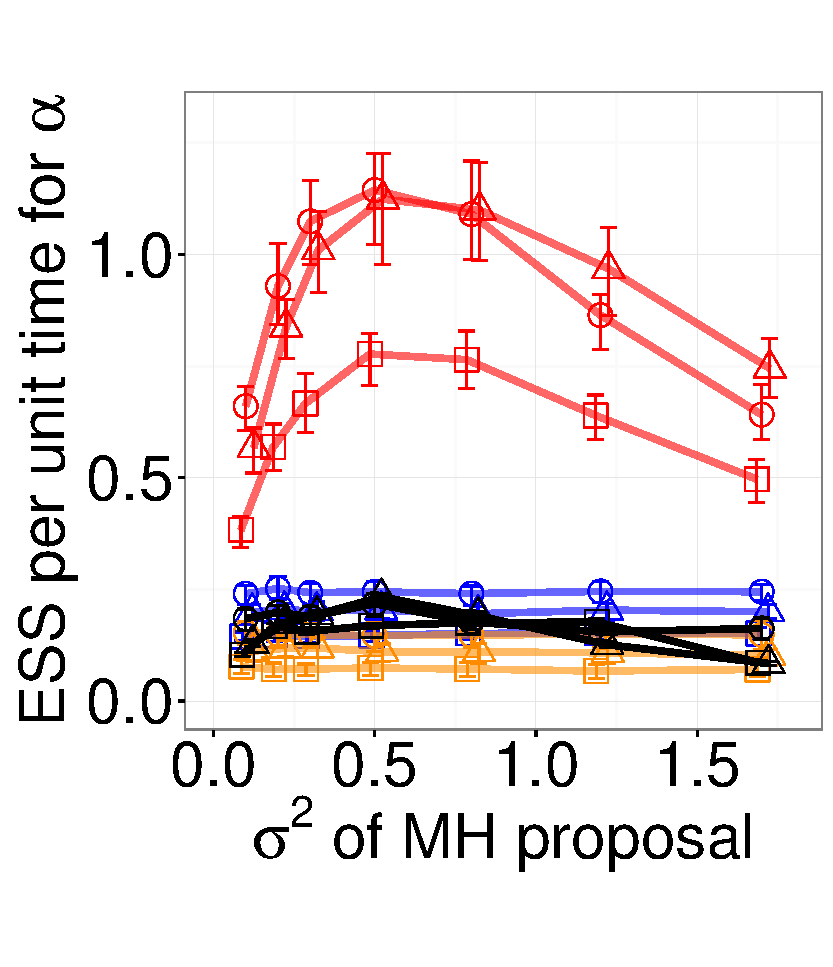
\includegraphics [width=0.45\textwidth, angle=0]{figures_new_apr12/exp_alpha_dim10_18apr12.pdf}
    \vspace{-0 in}
    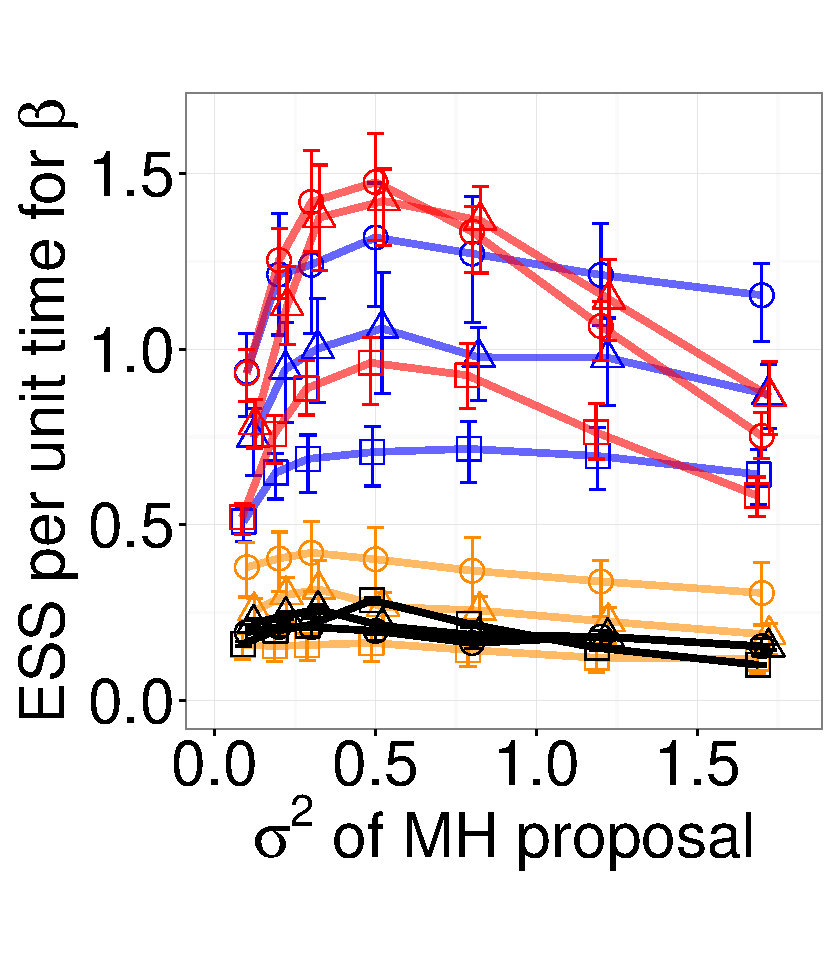
\includegraphics [width=0.45\textwidth, angle=0]{figures_new_apr12/exp_beta_dim10_18apr12.pdf}
    \vspace{-0 in}
  \end{minipage}
    \caption{ESS/sec for the synthetic  model, the top row being dimension 3, and the bottom,
      dimension 10. The left column is for $\alpha$, and the 
    right is for $\beta$. Red, yellow, blue and black curves are the symmetrized MH,
  \naive\ MH, Gibbs and particle MCMC algorithm. Different symbols correspond
to different settings of the algorithms, see section~\ref{sec:expts}}
     \label{fig:ESS_EXP_D10}
  \end{figure}
  Figure~\ref{fig:ESS_EXP_D10} plots the ESS per unit time for the parameters 
  $\alpha$ (left) and $\beta$ (right) for the
  case of $3$ states (top row) and $10$ states (bottom row) as we vary the scale-parameter $\sigma^2$ of the
  log-normal proposal distribution. We include results for $5$ states in the 
  supplementary material, the conclusions are the same. 
  %as we change the variance of the
  %proposal kernel, for different methods and different scaling parameters.
  %($\kappa =
%1.5, 2, 3$) and dimensions($p = 3, 5, 10$).
%, where   $k = 1.5$,  $\Omega(\theta, \theta^*) = k \max(\max A(\theta), \max A(\theta^*))$. 
%For particle MCMC, the number of particles can be $5, 10 , 20$. 
%  Blue lines are the Gibbs sampler, orange lines are \naive\ MH, red lines 
%are the symmetrized MH and black lines are particle MCMC. 
%For methods involving standard uniformization (Gibbs and \naive\ MH), dots 
%correspond to $\kappa = 1$, triangles correspond to $\kappa = 2$, and squares 
%correspond to $\kappa = 1.5$. For our symmetrized MH algorithm, circles,
%triangles and squares correspond to $\Omega = (\Omega_{old} + \Omega_{new}),
%2(\Omega_{old} + \Omega_{new})$ and $1.5 \max(\Omega_{old}, \Omega_{new})$
%respectively, where $\Omega_{new}$ and $\Omega_{old}$ equal $\max_i A_i$ under 
%the proposed and current parameters.
%  For particle MCMC, the dot-dashed lines correspond to 
%  $5$ particles,  the dashed lines correspond to $10$ particles, and the solid 
%  lines correspond to $20$ particles.
We see that our symmetrized MH algorithm is significantly more efficient 
than the baselines over a wide range of choices of $\sigma^2$, 
(including the natural choice of $1$).
Among the three setting of our algorithm, the simple additive setting
 ({triangles}) does best, though it is only slightly better than 
 the {max-of-max} setting (circles). {A possible reason for this improvement is 
  that the additive setting is more stable than the max-of-max setting, when the 
proposal variance can be large. The {additive setting with a multiplicative factor 
of $1.5$} (squares) does worse than both {additive choice with smaller multiplicative
factor and the max-of-max choice} but still better than the other algorithms. Among 
the baselines, simple Gibbs sampling 
does better than \naive\ Metropolis-Hastings, suggesting that the dependency of 
the Poisson grid on the MJP parameters does indeed significantly slow 
down mixing. Particle MCMC has the worst performance for this task. The
results in figure~\ref{fig:ESS_EXP_D10} for the 10-dimensional state space
show that for the parameter $\alpha$, the improvement that our proposed
sampler affords is even more dramatic. For the parameter $\beta$ however,
it's performance is comparable to Gibbs, although it's not possible to
claim one is uniformly superior to the other.

  \begin{figure}%[b]    
  \centering
  \begin{minipage}[hp]{0.24\linewidth}
  \centering
    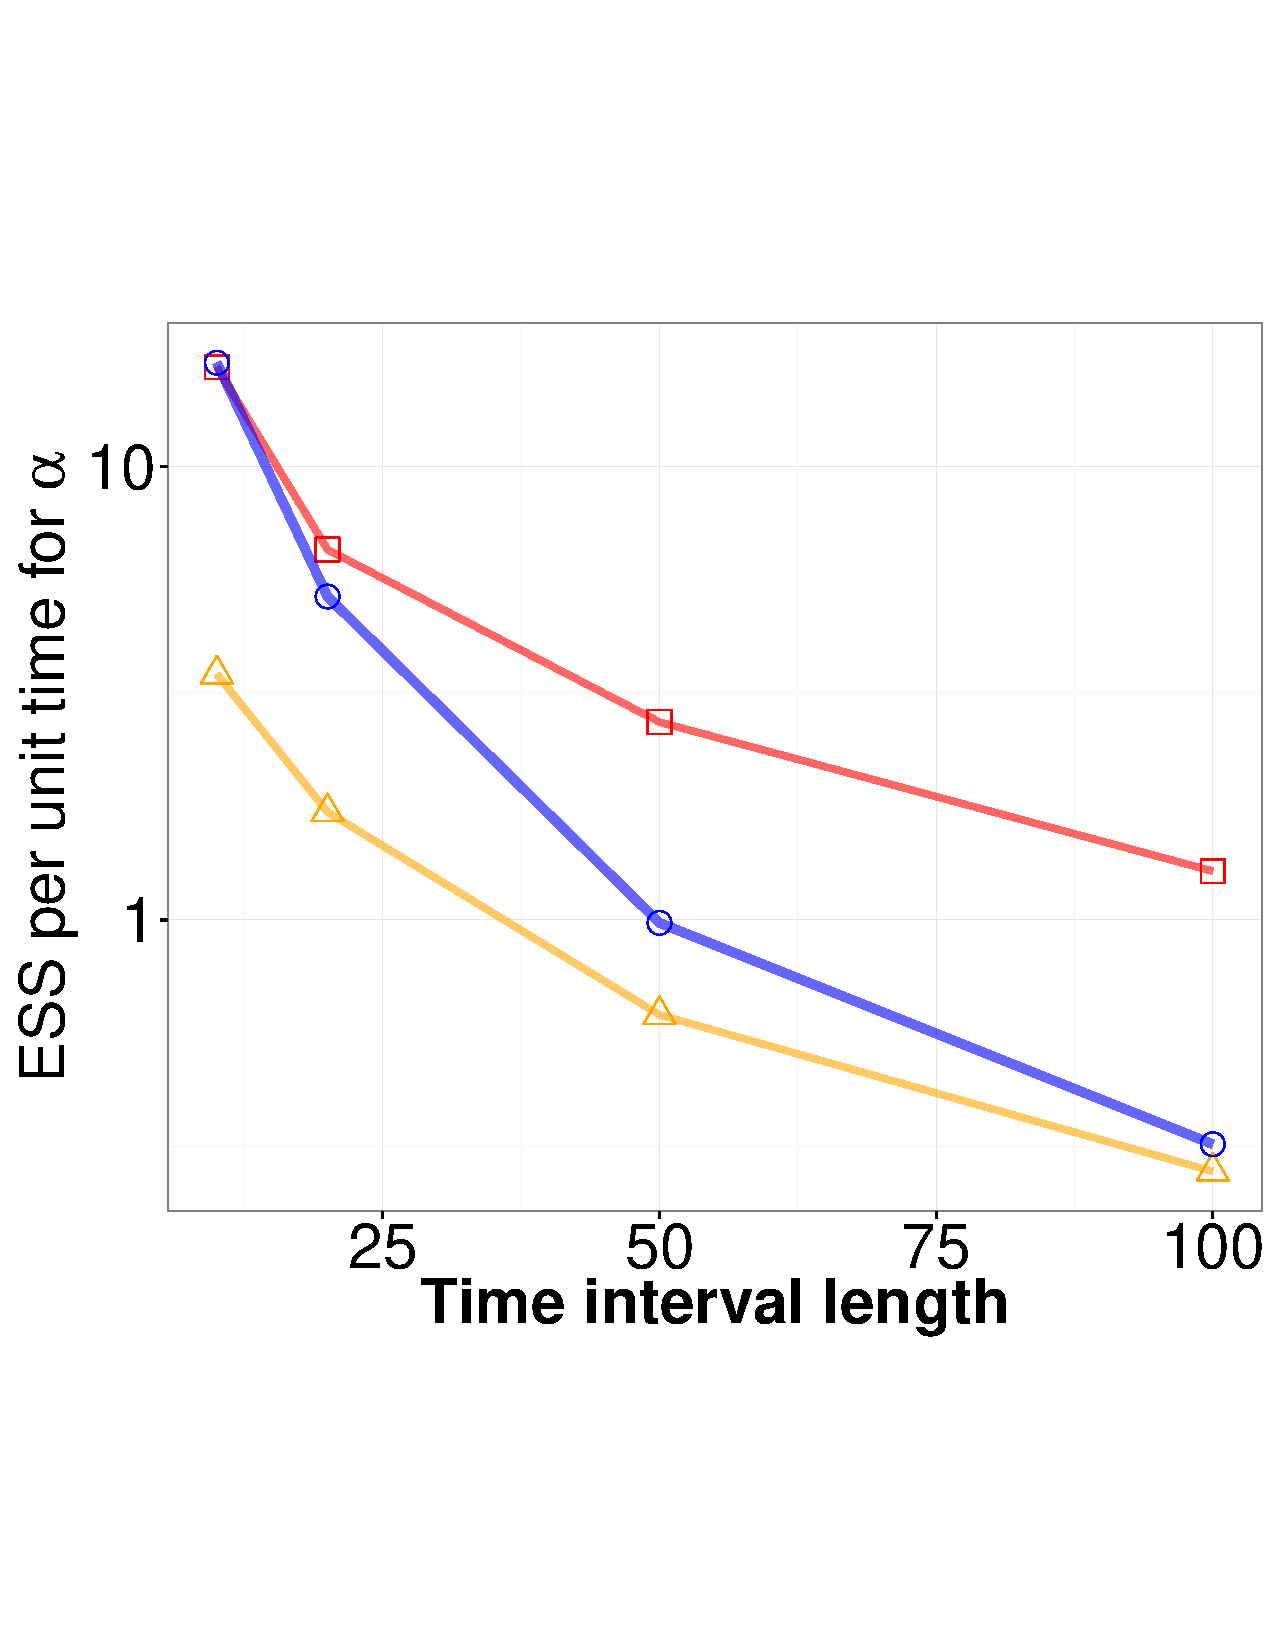
\includegraphics [width=0.99\textwidth, angle=0]{figs/ESS_vs_t_alpha_fixobservation.pdf}
    \end{minipage}
  \begin{minipage}[hp]{0.24\linewidth}
  \centering
    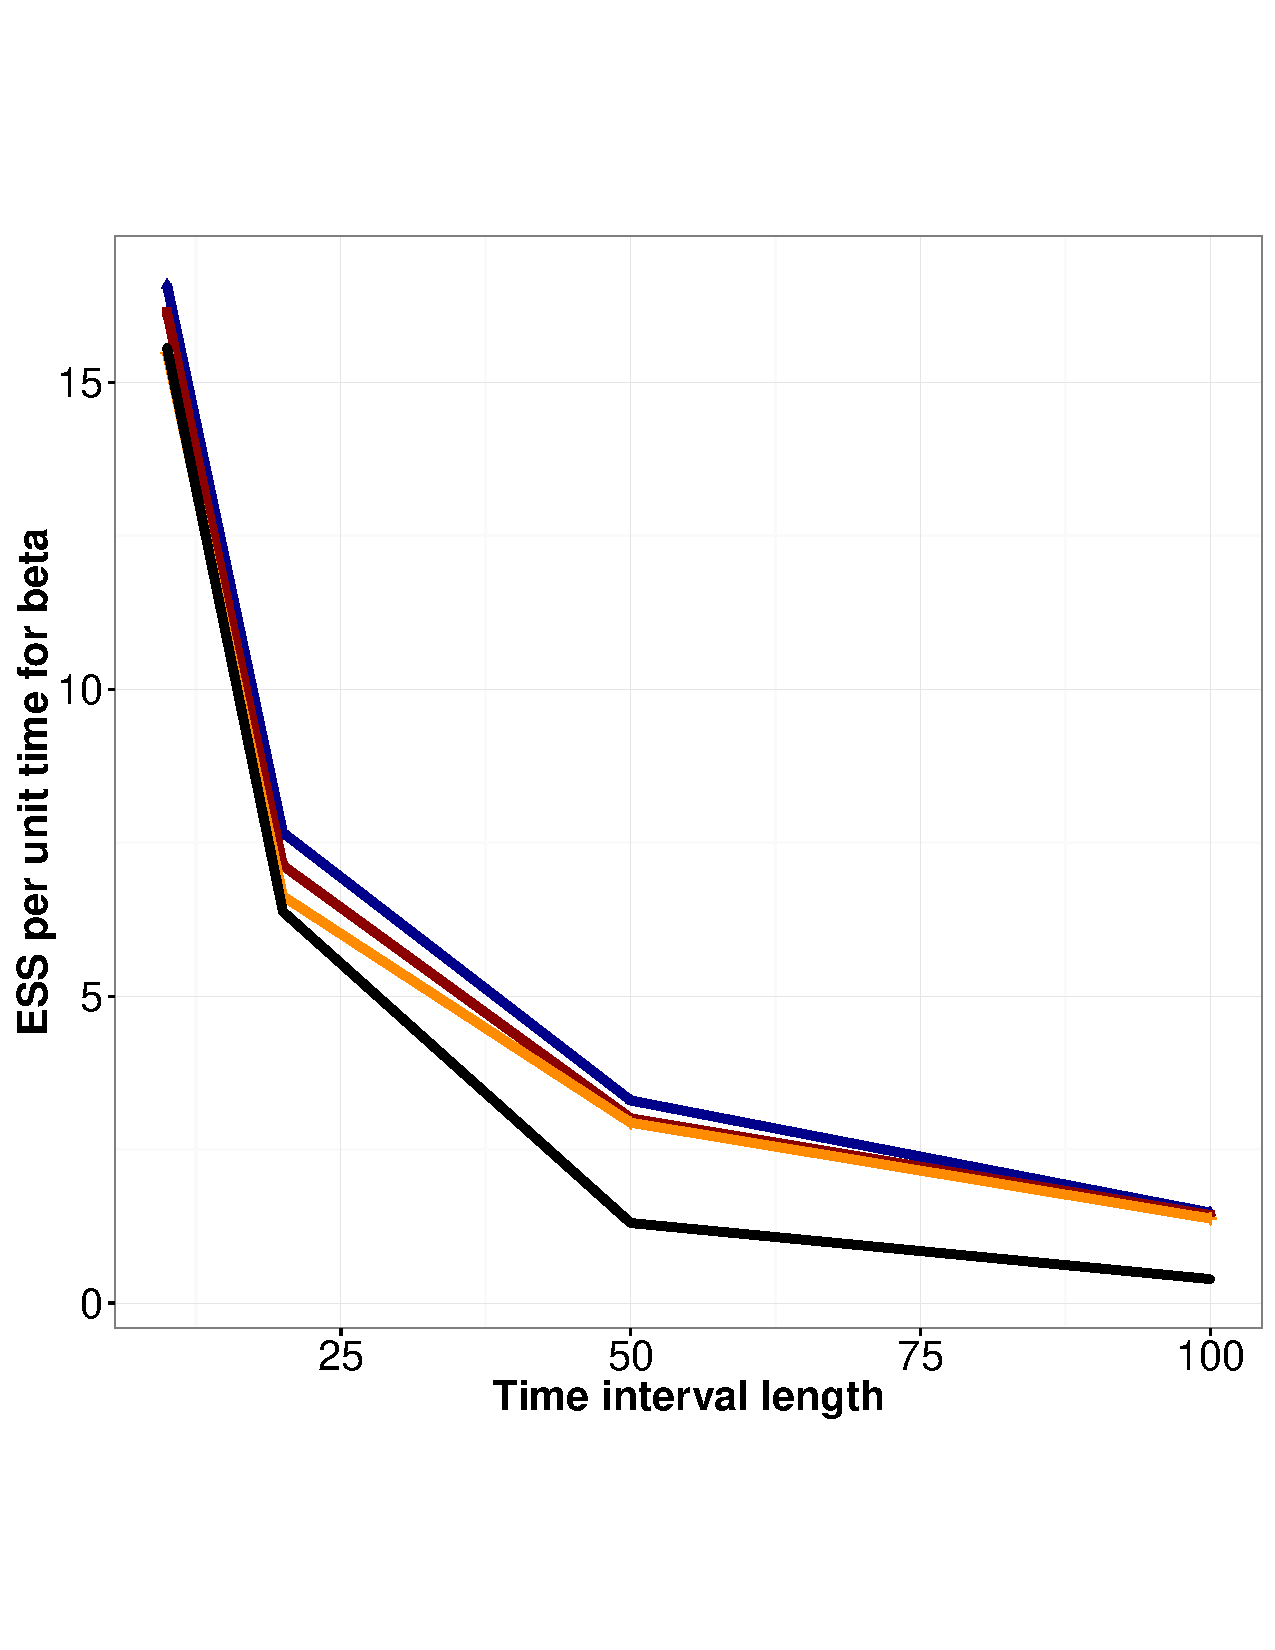
\includegraphics [width=0.99\textwidth, angle=0]{figs/ESS_vs_t_beta_fixobservation.pdf}
%    \vspace{-0.3in}
  \end{minipage}
    %\label{fig:TSS_fix}
  \begin{minipage}[hp]{0.24\linewidth}
  \centering
    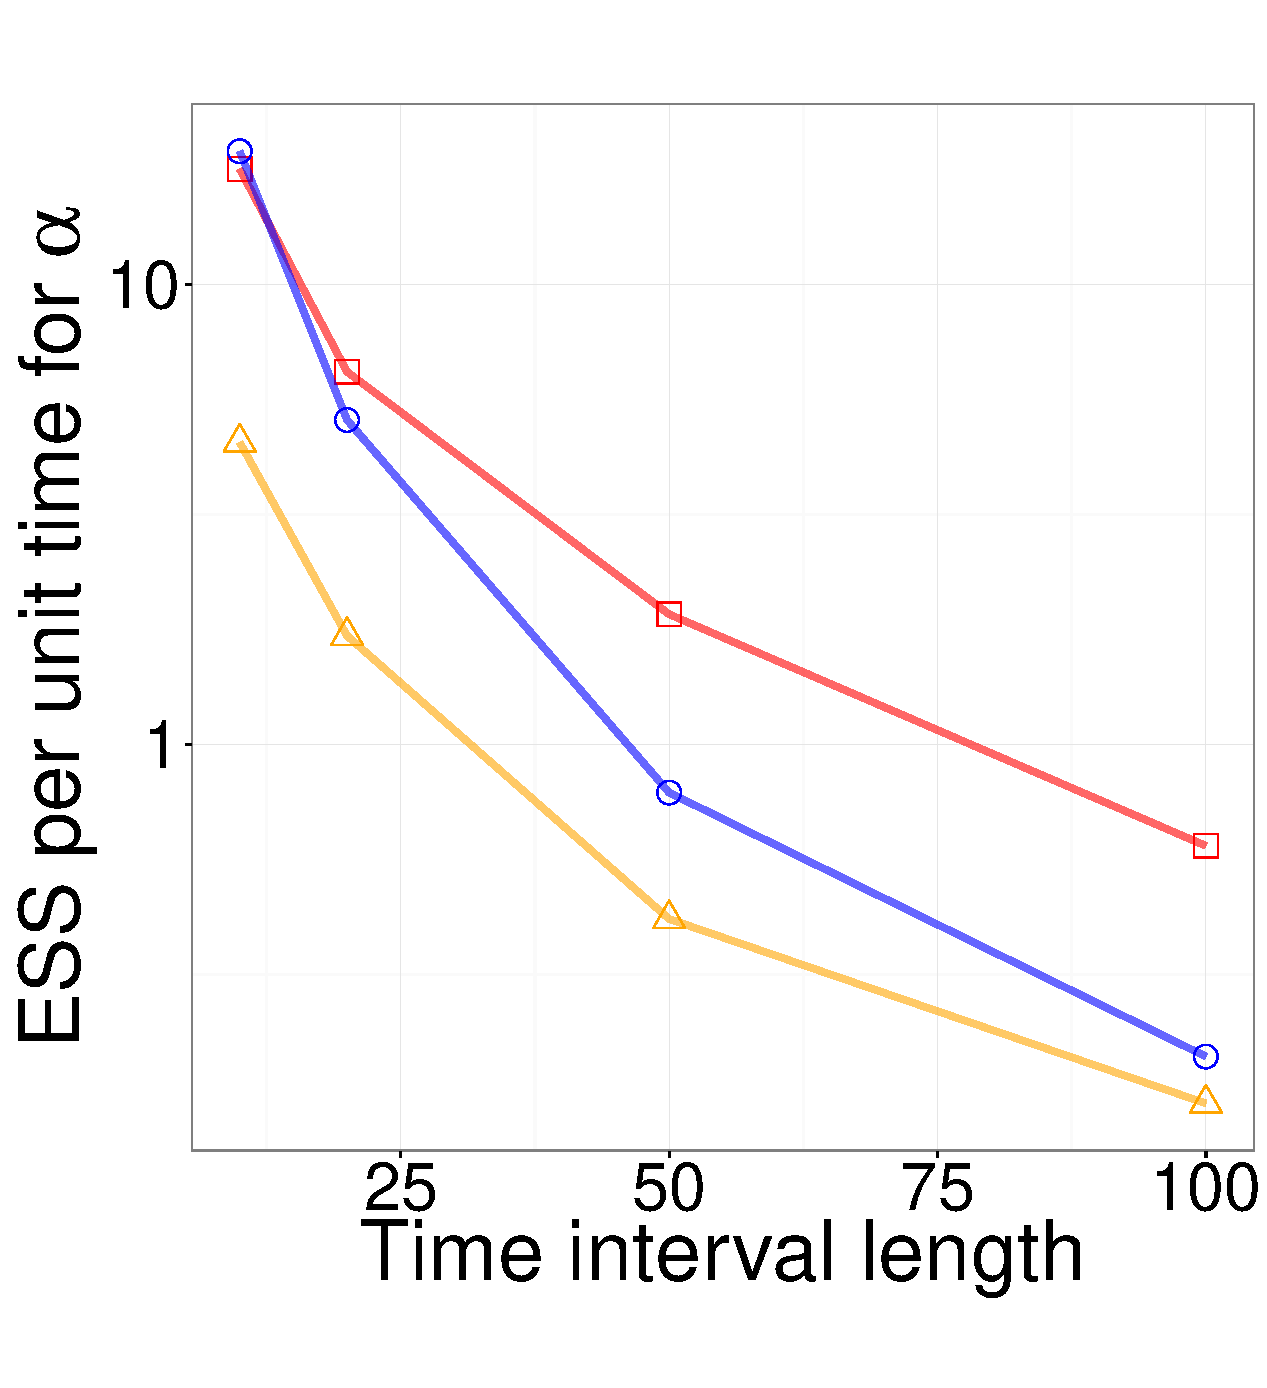
\includegraphics [width=0.99\textwidth, angle=0]{figs/ESS_vs_t_alpha.pdf}
      \end{minipage}
  \begin{minipage}[hp]{0.24\linewidth}
  \centering
    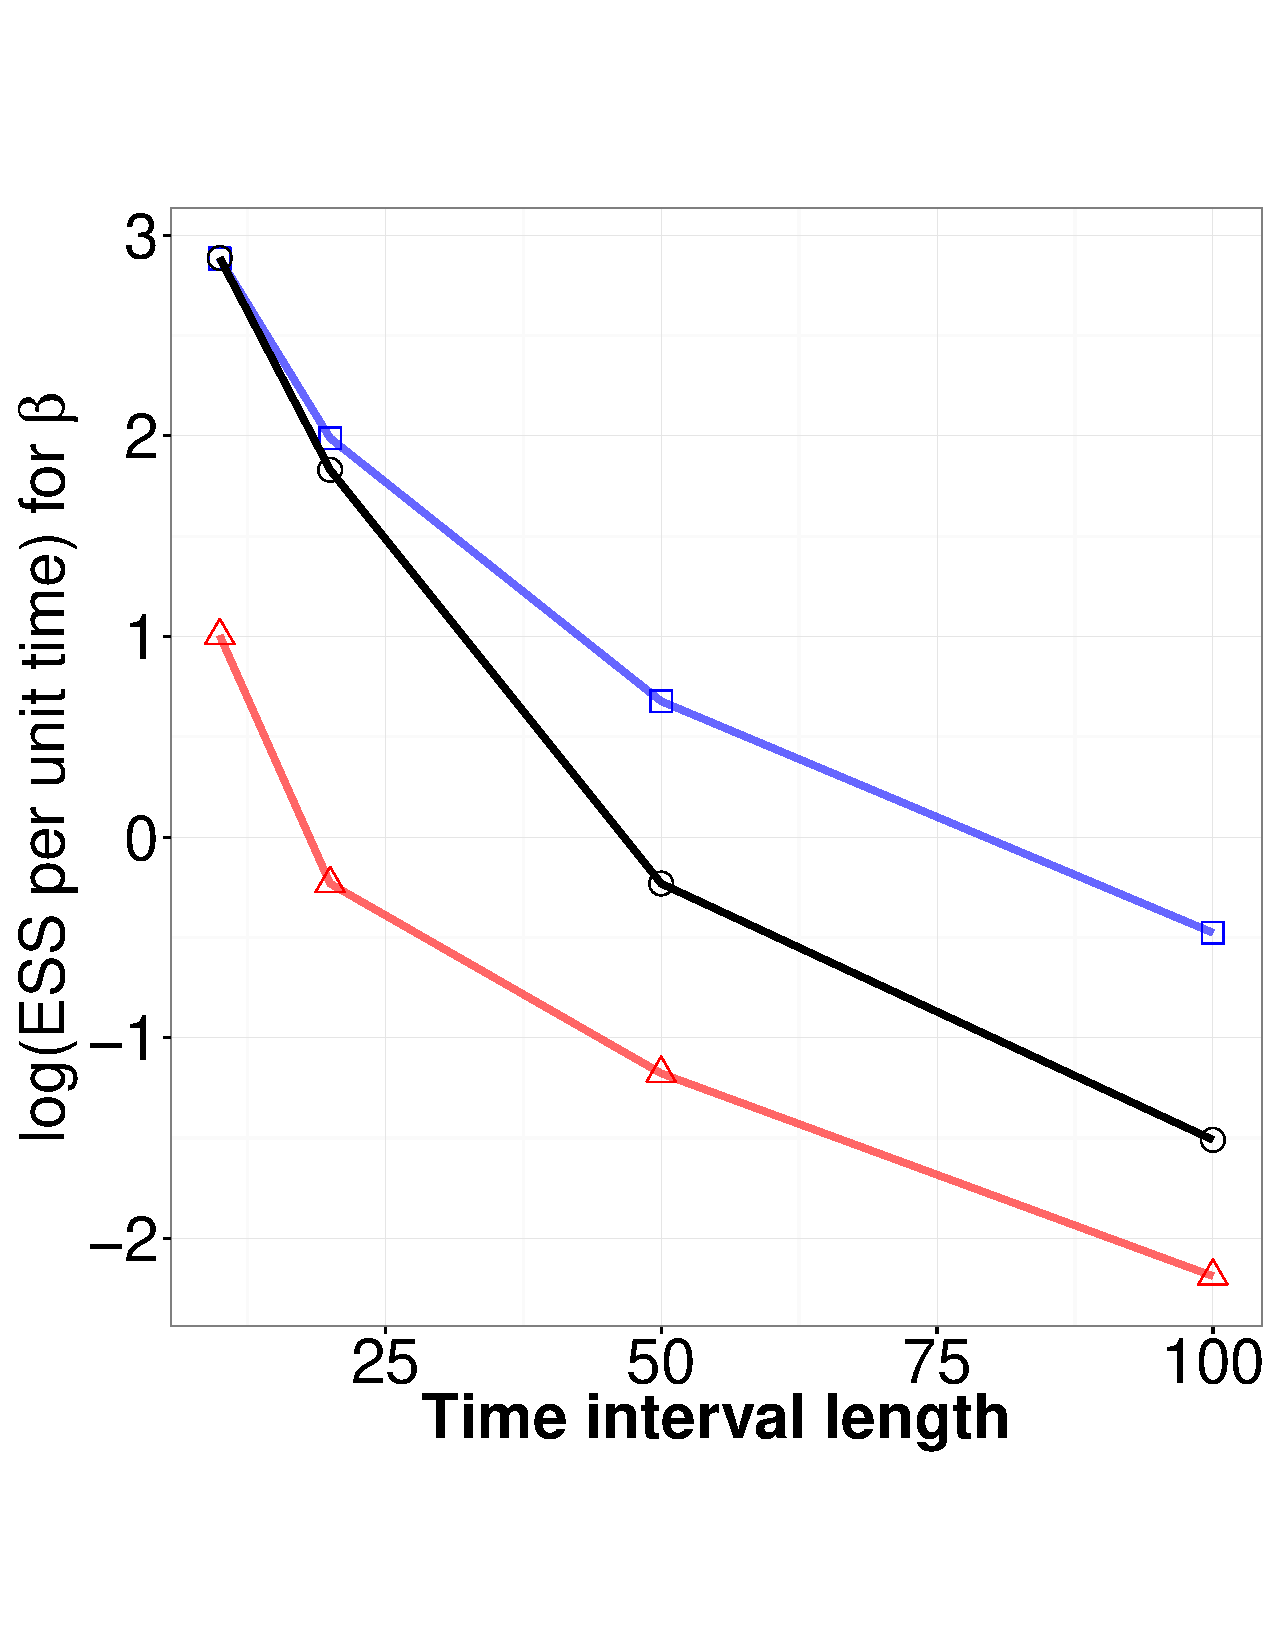
\includegraphics [width=0.99\textwidth, angle=0]{figs/ESS_vs_t_beta.pdf}
  \end{minipage}
%    \vspace{-0.3in}
%    \caption{Time Interval vs. ESS / sec}
    \caption{Time Interval vs. ESS/sec. In the left two plots, the number of 
    observations is fixed, in the right two, this grows linearly with the
  interval length. Red, yellow and blue curves are the symmetrized MH,
  \naive\ MH and Gibbs algorithm.}
     \label{fig:TSS}
  \end{figure}
%We generate different observations on different time intervals.
%Our observation process was a Gaussian distribution with mean equal to the 
%current state and variance equal to $1$. 
In figure~\ref{fig:TSS}, we plot ESS per unit time as the observation 
interval $\cT$ increases. We consider the three-state MJP, and as before there 
are $19$ observations uniformly located over a time interval $(0,\cT)$. We 
consider four settings, with $\cT$ equal to $10, 20, 50, 100$. For each, we 
compare our symmetrized MH sampler (with $\kappa$ set to $1$) with the Gibbs 
sampler (with $\kappa$ set to $2$). While the performance of the Gibbs sampler 
is comparable with our symmetrized algorithm for the smallest value of 
$\cT$, its performance is considerably worse for longer time-intervals. This is 
because of the conditional nature of the updates of the Gibbs sampler, where MJP
trajectories are sampled as intermediate objects to facilitate updating the
parameters. Longer time intervals will then result in stronger coupling between 
MJP path and parameters, slowing down mixing. This effect disappears if we 
integrate out the MJP trajectory. This experiment demonstrates that it
is not sufficient just to integrate out the state values of the trajectory, 
instead, we also have to get around the effect of the
trajectory transition times. Our symmetrized MH-algorithm allows us to do
this. 
%as a by-product, it also involves calculating a simpler 
%MH acceptance probability.


In figure~\ref{fig:TSS}, we plot results from a similar experiment. Now,
instead of keeping the number of measurements fixed as we increase the 
observation interval, we keep the observation rate fixed at one observation 
every unit interval of time, so that longer observation intervals have larger 
number of observations. The results are similar to the previous case: Gibbs 
sampling performs well for small observation intervals, with performance 
degrading sharply for larger observation intervals. These two experiments 
illustrate the usefulness of our idea of integrating out the MJP path while 
carrying out parameter inference.

  \subsection{The Jukes and Cantor (JC69) model}~
  \begin{figure}%[H]
  \centering
  \begin{minipage}[!hp]{0.7\linewidth}
  \centering
    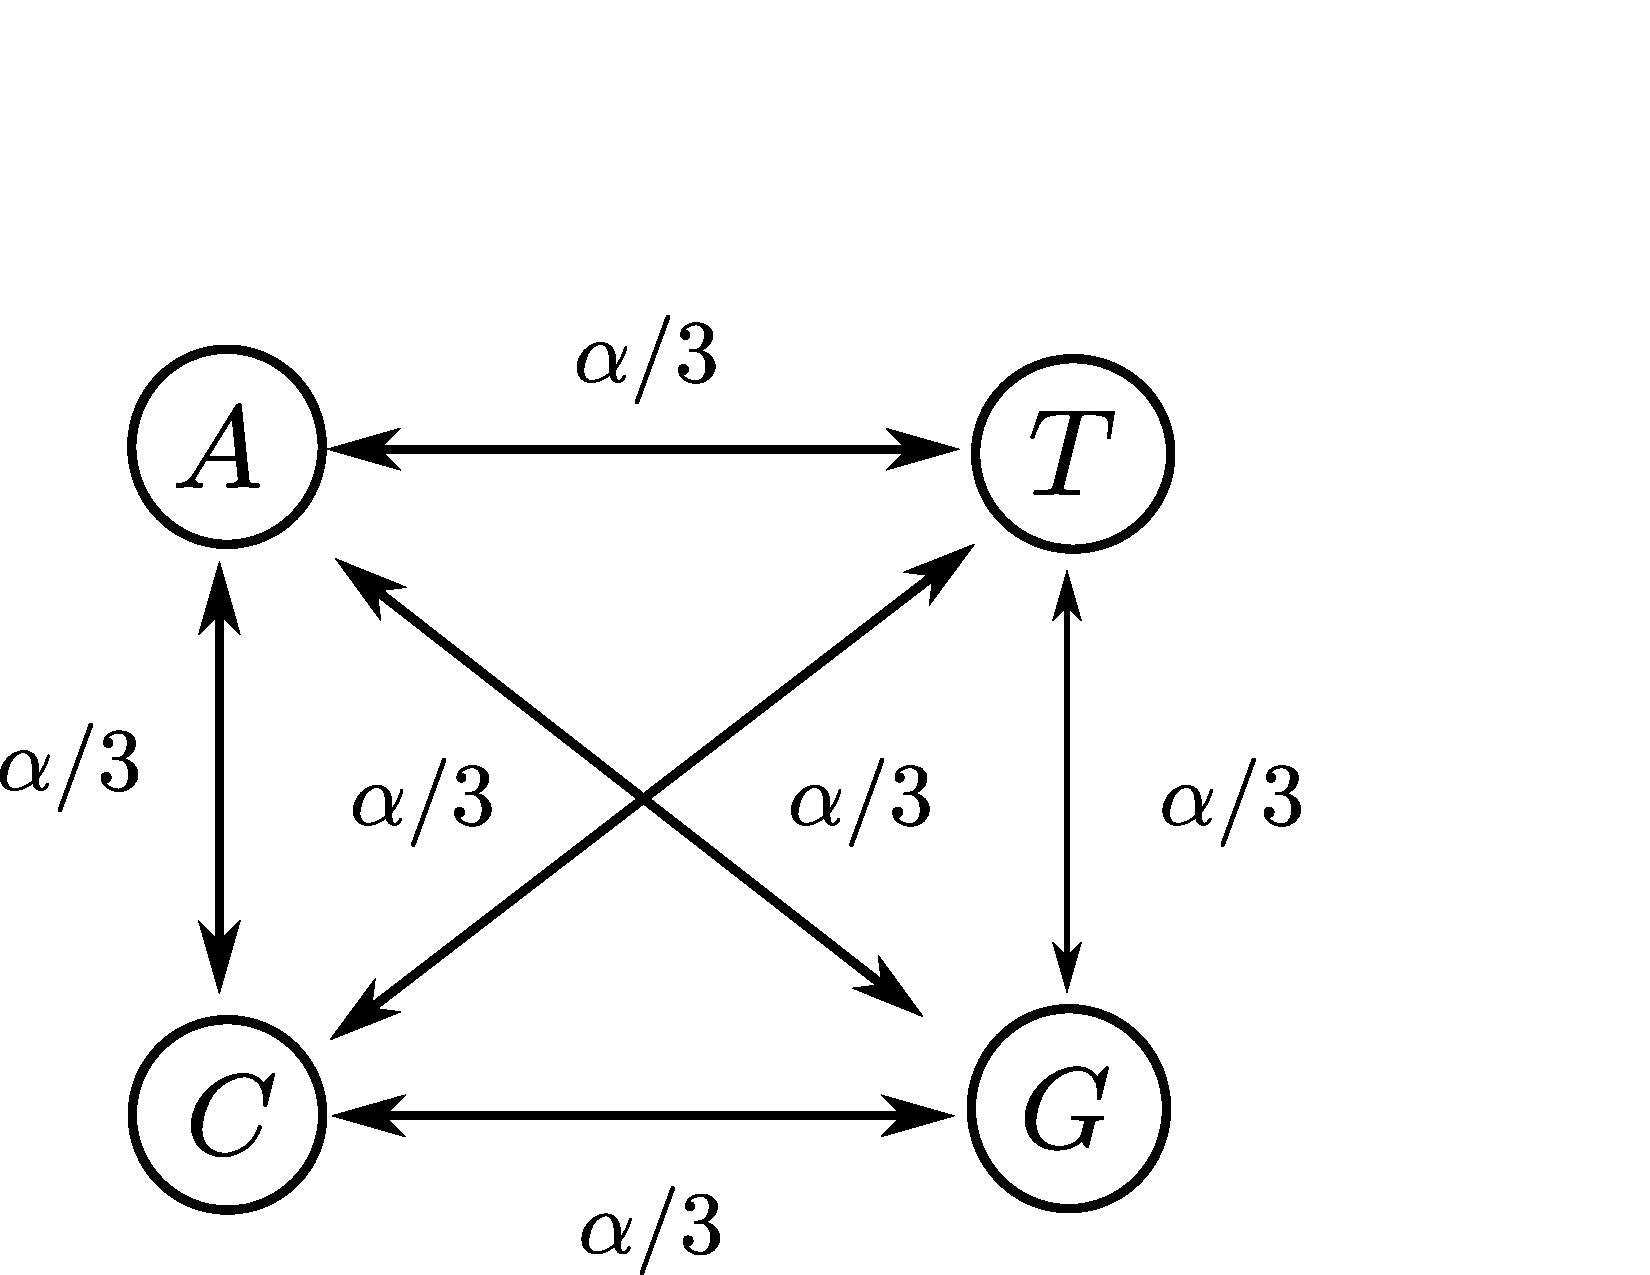
\includegraphics[width=.45\textwidth, angle=0]{figs/jc_model.pdf}
    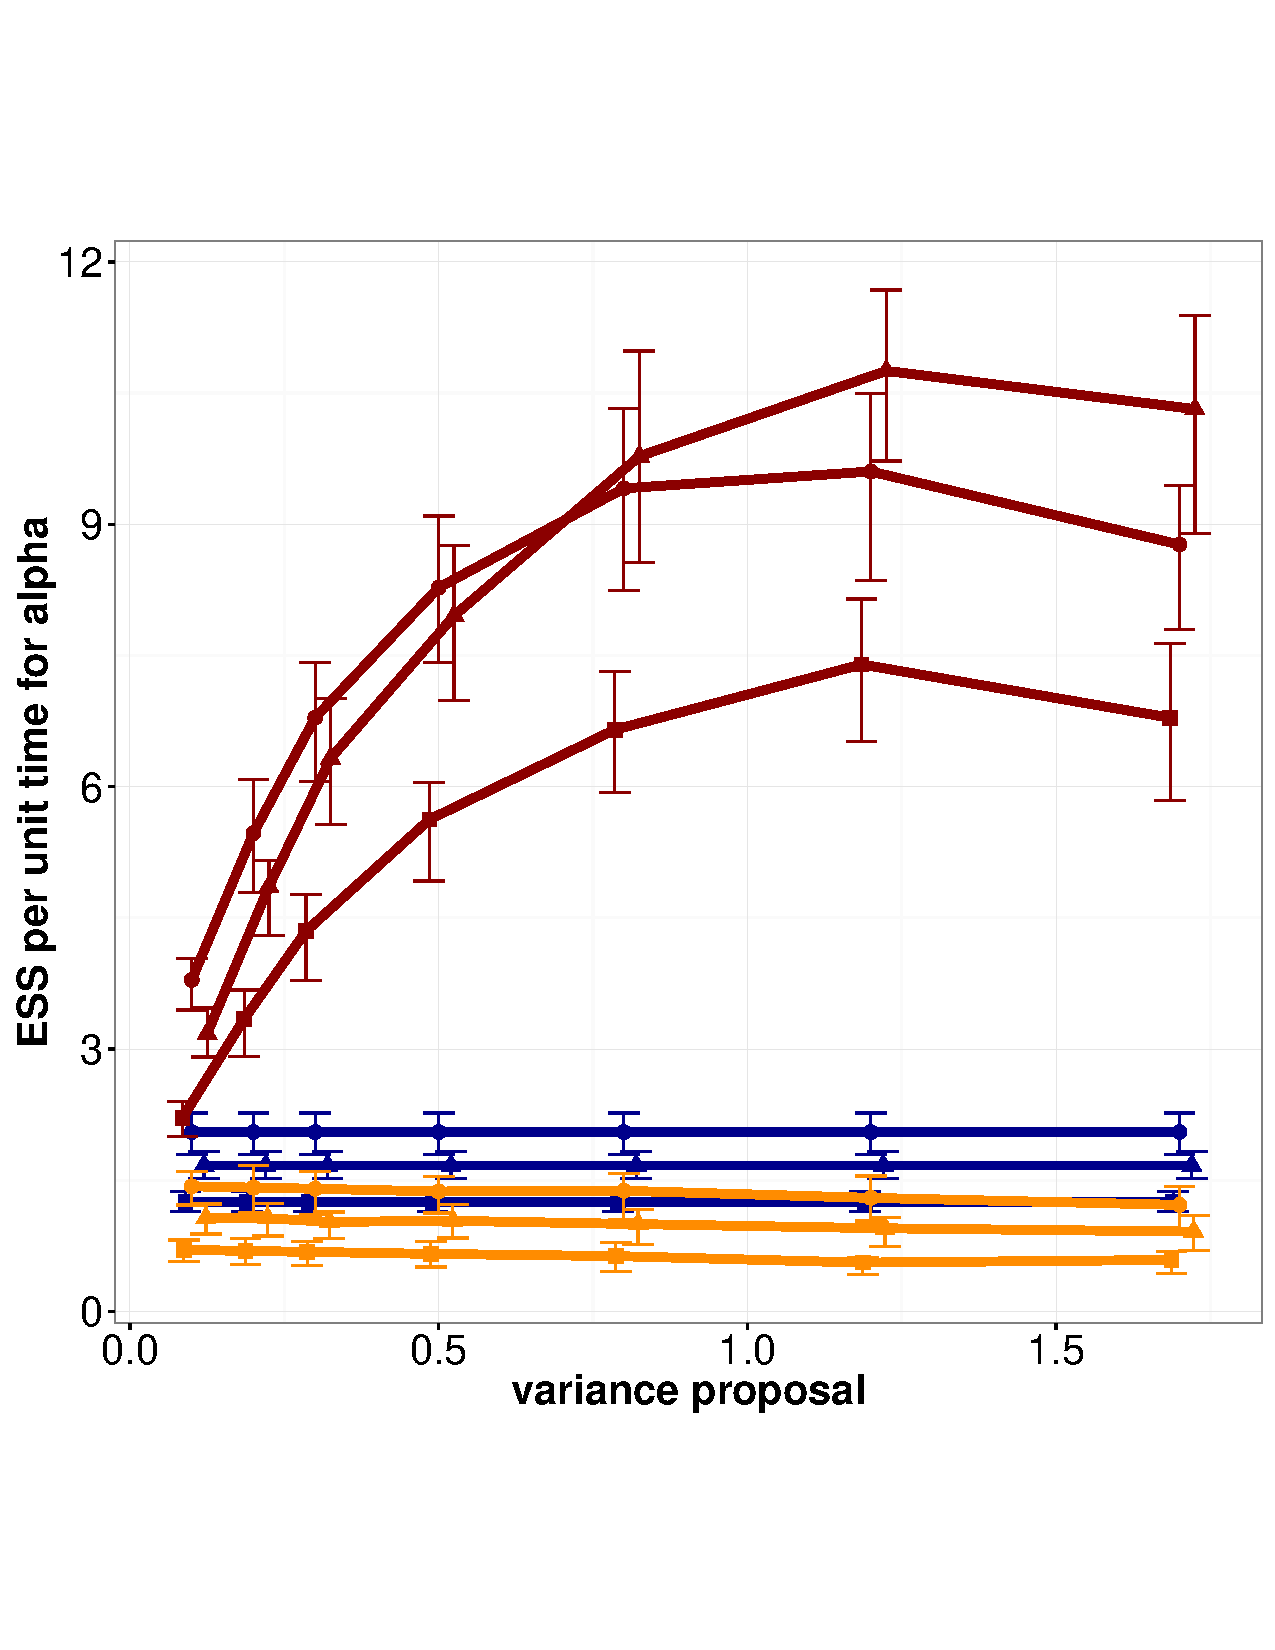
\includegraphics[width=0.45\textwidth, angle=0]{figs/jc.pdf}
	%\label{jc_model}
     \label{fig:ESS_JC}
  \end{minipage}
  \begin{minipage}[!hp]{0.28\linewidth}
  \caption{(a) Jukes-Cantor (JC69) model, (b)
    ESS/sec for the JC69 Model. Red, yellow and blue curves are the 
      symmetrized MH, \naive\ MH and Gibbs algorithm. }
  \end{minipage}
  \end{figure}
  The Jukes and Cantor (JC69) model is a popular model of DNA nucleotide
  substitution.  We write its state space as $\{0, 1, 2, 3\}$, representing the 
  four nucleotides $\{A, T, C, G\}$.  The model has a single parameter $\alpha$, 
  representing the rate at which the system transitions between any pair of 
  states. Thus, the rate matrix $A$ is given by 
  %Assume: $S = [S_0,S_1, ...,S_N] \;, T = [t_0(t_{start}), t_1,...,t_N, t_{N+1}(t_{end})]$, and y as observations.\\
$A_i = -A_{i,i} = 3\alpha, A_{i, j} = \alpha,i \neq j.$
We place a Gamma$(3,2)$ prior on the parameter $\alpha$.
Figure~\ref{fig:ESS_JC}(right) compares different samplers: we see that the
symmetrized MH samplers comprehensively outperforms all others.
Part of the reason why the difference is so dramatic here is because the
transition matrix is no longer sparse in this example, implying a stronger
coupling between MJP path and parameter $\alpha$. We point out that for Gibbs
sampling, the conditional parameter update is conjugate, and there is no
proposal distribution involved (hence it's performance remains fixed along
the x-axis). Particle MCMC performs worse
than all the algorithms, and we do not include it in our plots.

In figure~\ref{fig:jc_model_vs_t}, we plot the ESS per unit time for the
different samplers as we increase the observation interval. In the left plot,
we keep the number of observations fixed, in the right, these increase with
the observation interval. Once again we see that our proposed algorithm
1) performs best over all interval lengths, and 2) suffers a performance
degradation with interval length that is much milder than the other algorithms.
%$$p(\alpha) = \frac{\lambda^\mu}{\Gamma(\mu)}\alpha^{\mu -1}e^{-\lambda \alpha} $$.
%Then we can get the posterior distribution $$f(\alpha | s_0,S,T)$$ as follows.
%$$ f(\alpha| s_0,S,T) \propto \exp(-(\lambda + 3(t_{end} - t_{start}))\alpha) \alpha^{\mu + N -1} .$$
%$\alpha | s_0,S,T$ is following $Gamma(\mu+ N,\lambda + 3(t_{end} - t_{start}))$\\
  \begin{figure}%[H]
  \centering
  \begin{minipage}[!hp]{0.73\linewidth}
  \centering
    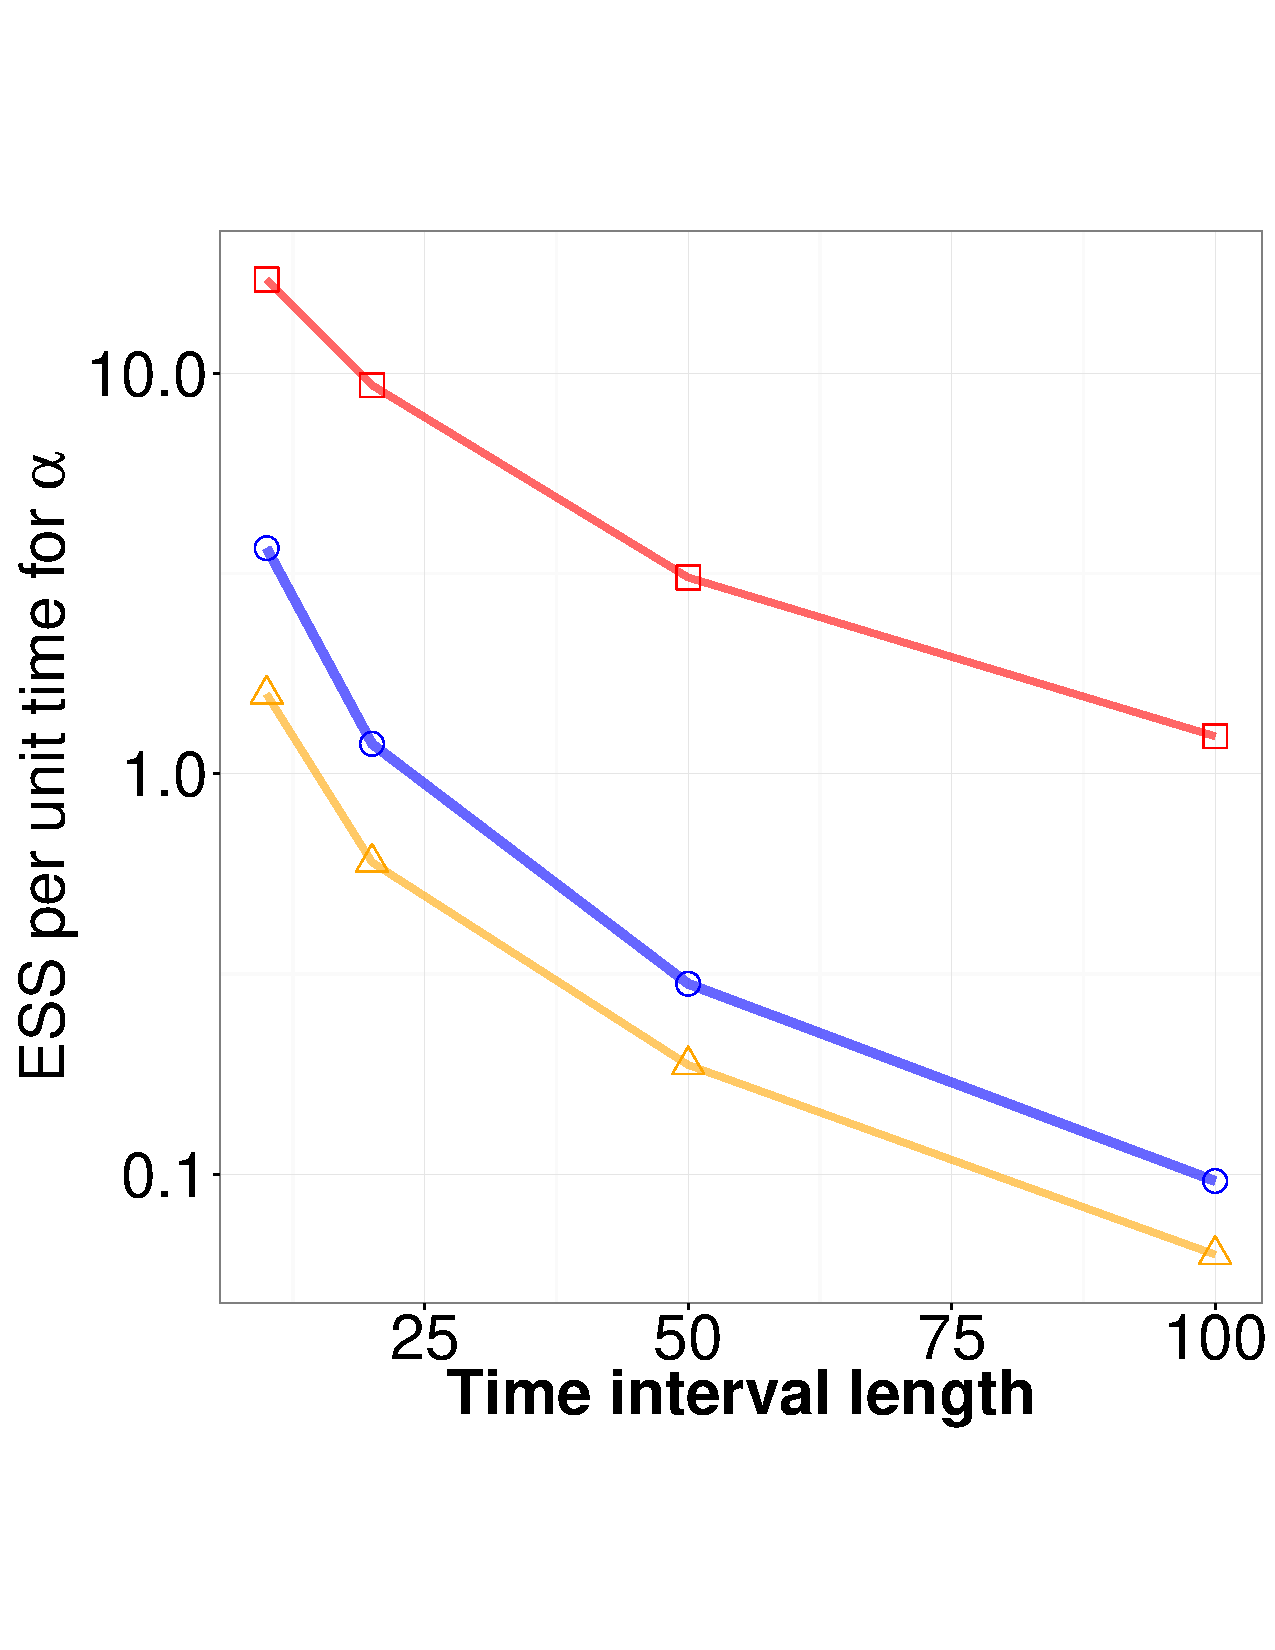
\includegraphics [width=0.45\textwidth, angle=0]{figs/ESS_vs_t_alpha_JC.pdf}
  \centering
    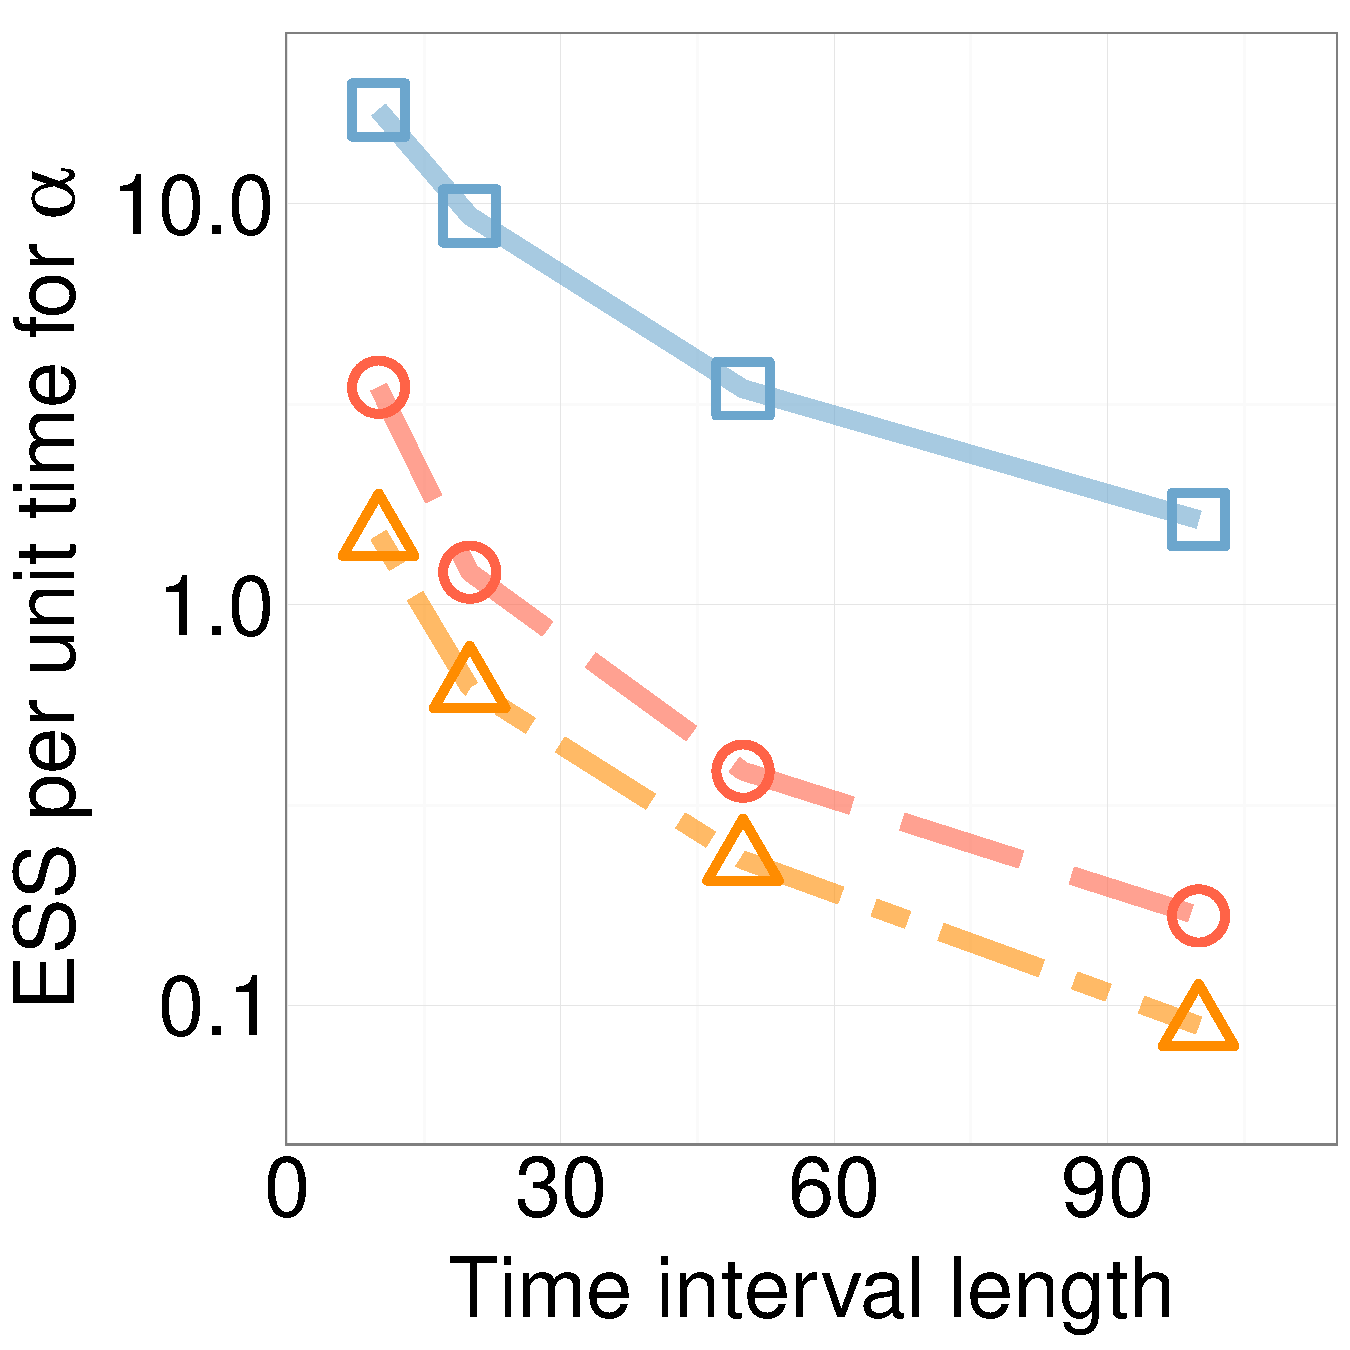
\includegraphics [width=0.45\textwidth, angle=0]{figs/ESS_vs_t_alpha_fixobservation_JC.pdf}
  \end{minipage}
  \begin{minipage}[!hp]{0.25\linewidth}
  \vspace{-.4in}
    \caption{Time Interval vs. ESS/sec. In the left plot, the number of 
    observations is fixed, in the right, this grows linearly with the
  interval length. Red, yellow and blue curves are the symmetrized MH,
  \naive\ MH and Gibbs algorithm. }
	\label{fig:jc_model_vs_t}
  \end{minipage}
  \end{figure}


\subsection{An immigration model with finite capacity}\label{sec:immig}~
Finally, we consider an M/M/N/N queue. This is a stochastic 
process whose state space is the set $\{0, 1, 2, 3, \cdots, N - 1\}$ with 
elements giving the number of customers/jobs/individuals in a system/population. 
Arrivals follow a rate-$\alpha$ Poisson process, moving the process from state 
$i$ to $i+1$ for $i<N$. The system has a capacity of $N$, so any arrivals when 
the current state is $N$ are discarded.  Service times or deaths are 
exponentially distributed, with a rate that is now state-dependent:
the system moves from $i$ to $i - 1$ with rate $i\beta$. 
%There are $N$ servers, which serve from the front of the queue. 
%If there are less than $N$ jobs, some of the servers will be idle. 
%Only $N$ customers can queue at any one time. 
%Any further arrivals to the queue are considered ''lost''. 

% \begin{figure}
% \centering
% \begin{minipage}[hp]{0.6\linewidth}%0.45
% \centering
%   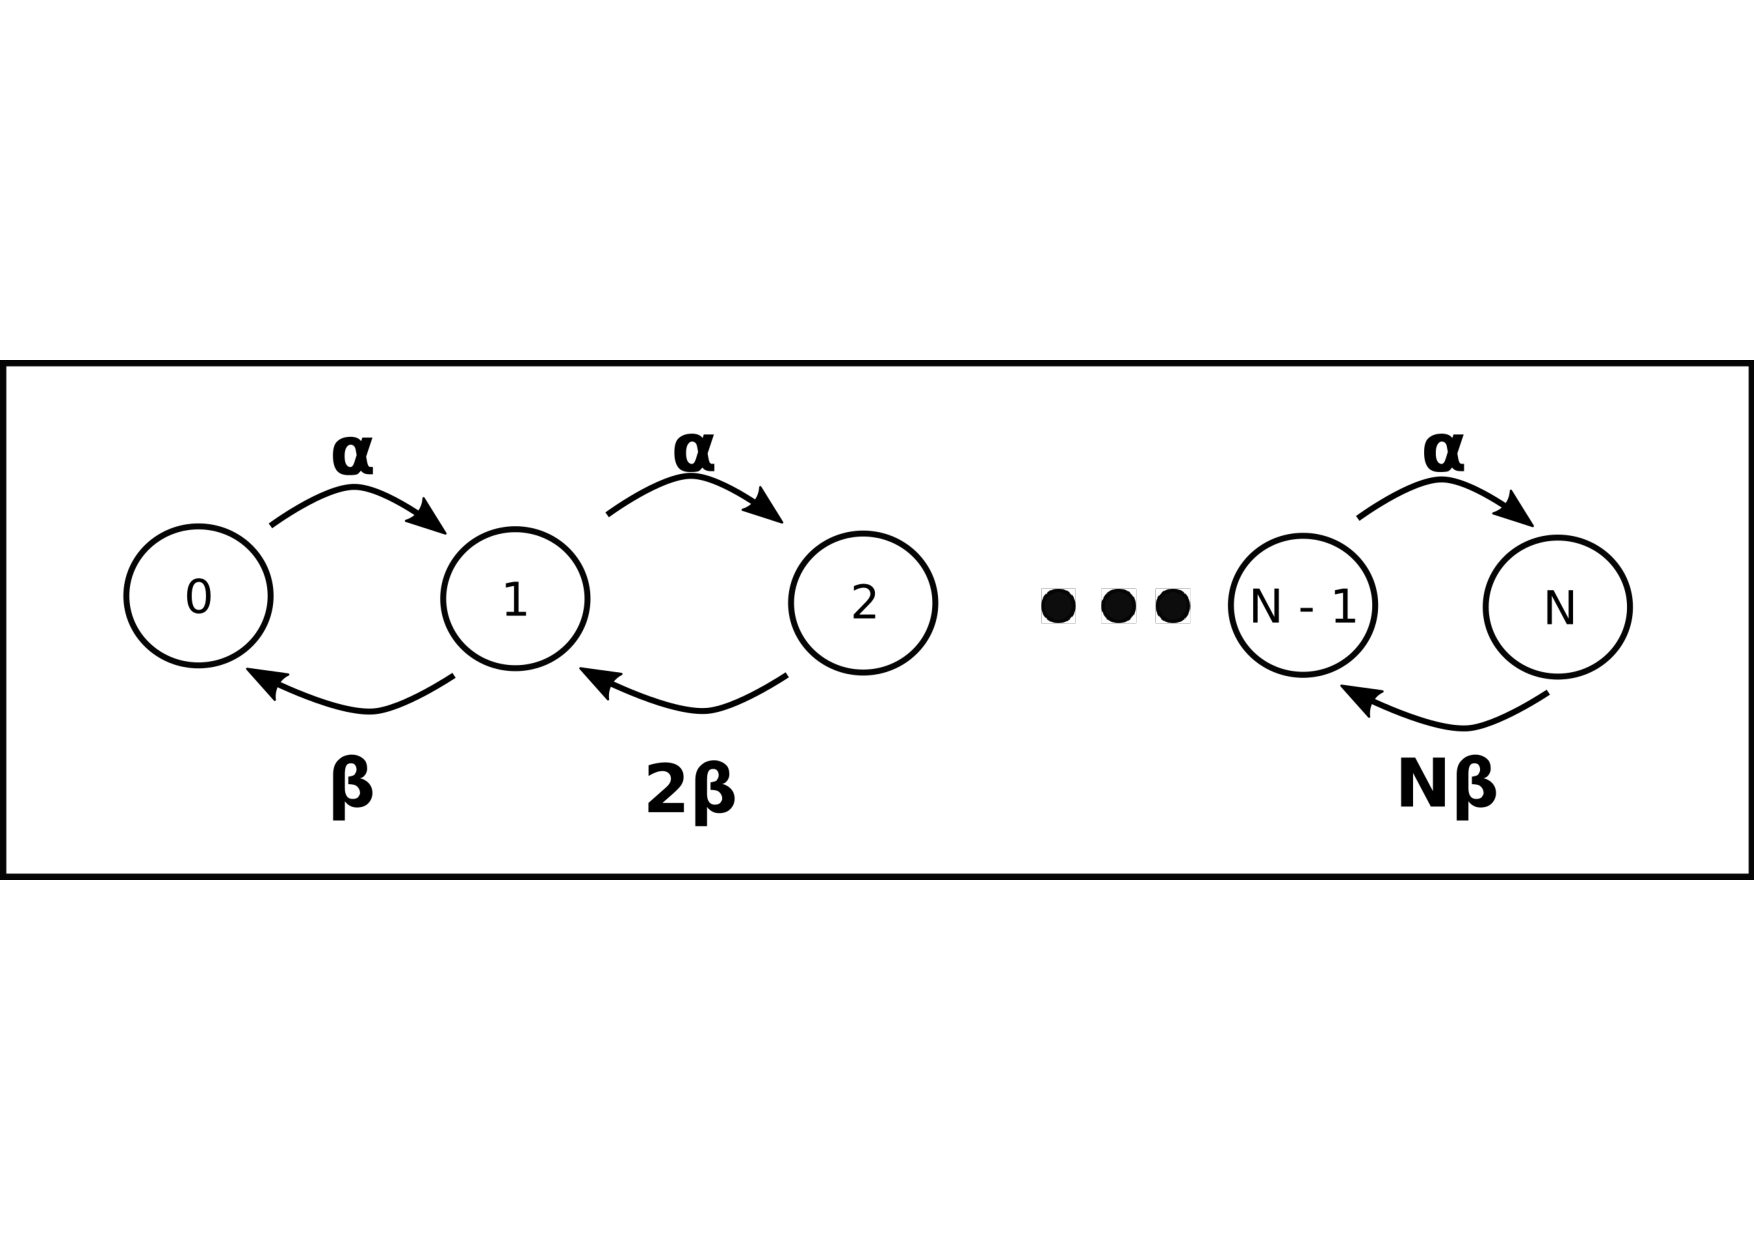
\includegraphics [width=1\textwidth, angle=0]{figs/queue_model.pdf}%0.70
%     \end{minipage}
%   \caption{queuing model}
%   \label{q_model}
% \end{figure}
  \begin{figure}%[b]
  \centering
  \begin{minipage}[hp]{0.82\linewidth}
  \centering
    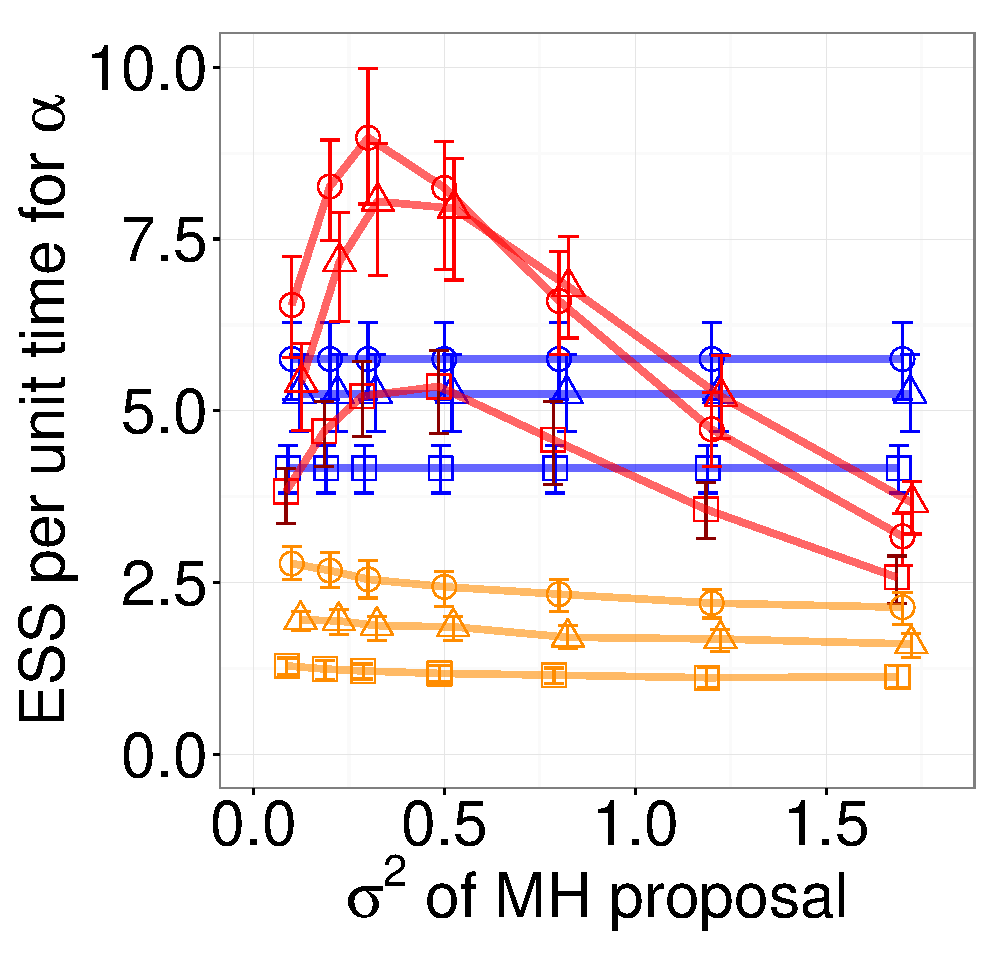
\includegraphics [width=0.48\textwidth, angle=0]{figures_new_apr12/Q_alpha_dim3_18apr12.pdf}
    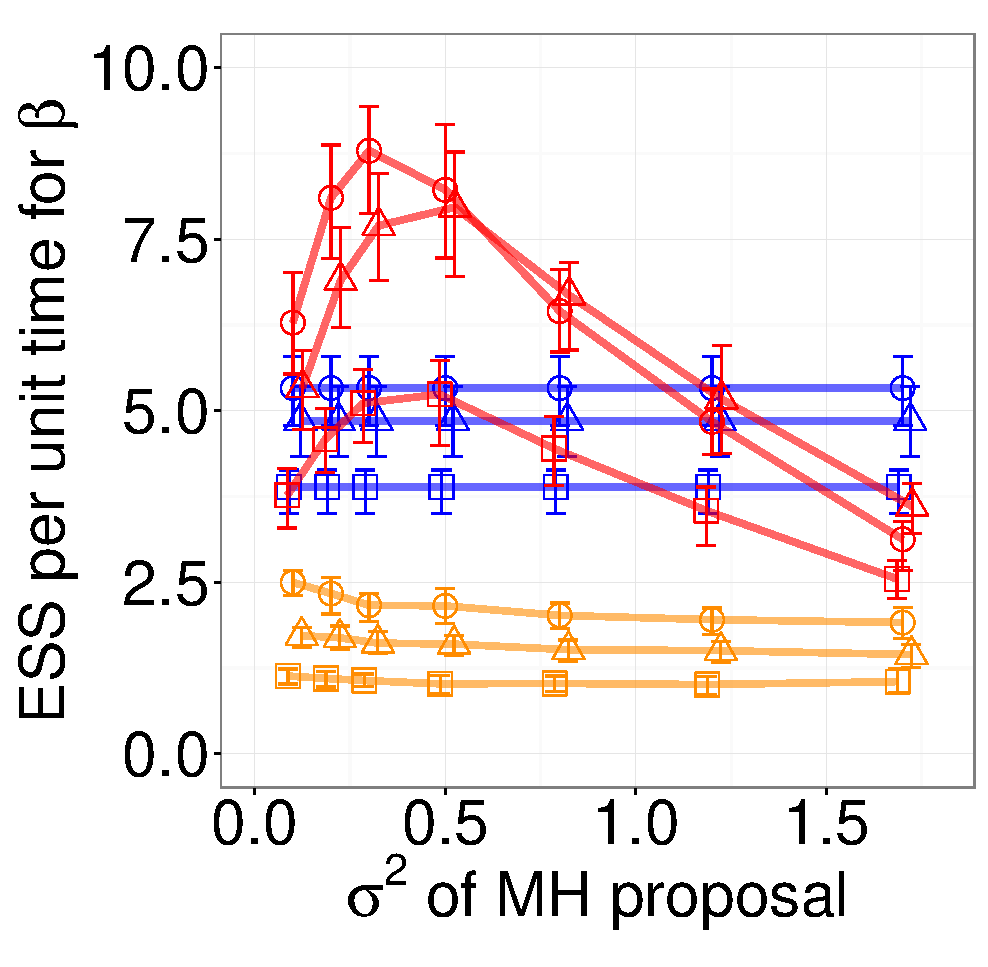
\includegraphics [width=0.48\textwidth, angle=0]{figures_new_apr12/Q_beta_dim3_18apr12.pdf}
%    \vspace{-1.0 in}
  \centering
    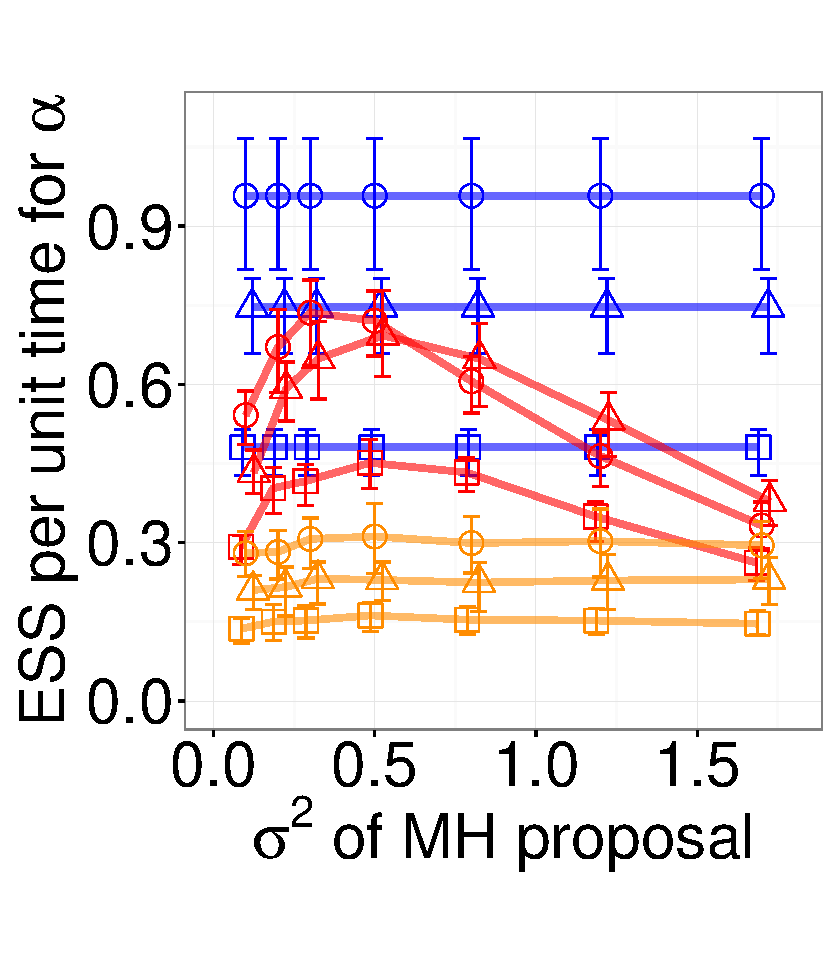
\includegraphics [width=0.48\textwidth, angle=0]{figures_new_apr12/Q_alpha_dim10_18apr12.pdf}
    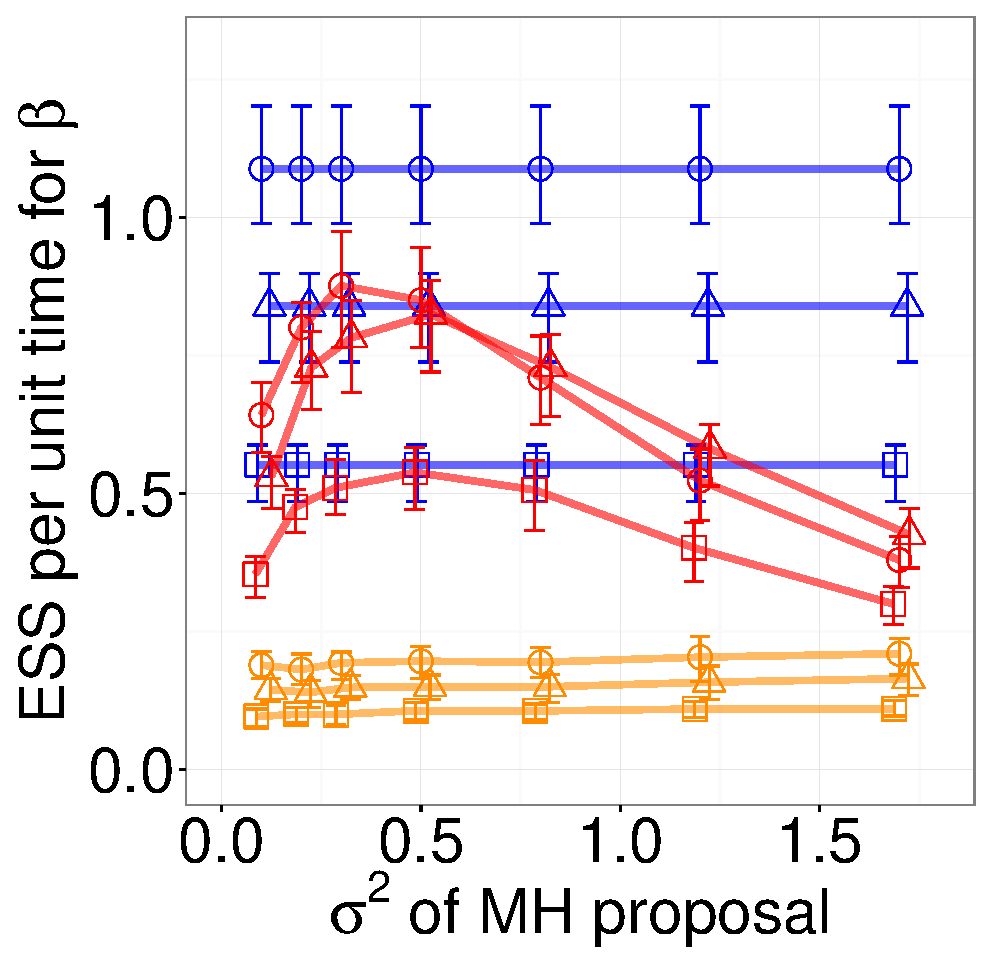
\includegraphics [width=0.48\textwidth, angle=0]{figures_new_apr12/Q_beta_dim10_18apr12.pdf}
 %   \vspace{-0.5 in}
  \end{minipage}
  \begin{minipage}[!hp]{0.17\linewidth}
    \caption{ESS/sec for the immigration model, the top row being dimension 3, and the bottom,
      dimension 10. The left column is for $\alpha$, and the 
    right is for $\beta$. Red, yellow, and blue curves are the symmetrized MH,
  \naive\ MH, Gibbs sampling and particle MCMC.}
     \label{fig:ESS_Q_D10}
  \end{minipage}
  \end{figure}
We follow the same setup as the first experiment:
for $(\alpha_0,\alpha_1,\beta_0,\beta_1)$ equal to $(3,2,5,2)$,
we place Gamma$(\alpha_0,\alpha_1)$, and Gamma$(\beta_0, \beta_1)$ priors on 
$\alpha$, $\beta$. These prior distributions are used to sample transition 
matrices $A$, which, along with a uniform distribution over initial states,
are used to generate MJP trajectories. We observe these at integer-valued
times according to a Gaussian observation process.
We consider three settings: $3, 5$ and $10$ states, with results from $5$ 
steps included in the supplementary material. 

  %\subsection{Experiments}
  Figure~\ref{fig:ESS_Q_D10} plots the ESS 
  per unit time for the parameters $\alpha$ (left) and $\beta$ (right) as we 
  change the variance of the proposal kernel, for different settings of
  different algorithms. The top row shows results for a state-space
  of dimension $3$, and the bottom row, results for a dimension
  $10$ (we include the case of dimension $5$ in the supplementary material).
  %Colors and types are the same as the previous experiment.
  Again, our symmetrized  MH algorithm does best for dimensions
  $3$ and $5$, although now Gibbs sampling performs well for dimensionality $10$.
  This is partly because for the problem, the Gibbs conditionals over $\alpha$
  and $\beta$ and conjugate, and have a very simple Gamma distribution
  (this is also why the Gibbs sampler curves are straight lines: there is no
  proposal distribution involved here).
% Figure~\ref{fig:hist} shows posterior distributions for 
% $P(\theta | X)$(red), $P(\theta | S, T, X)$(green), $P(\theta | W, X)$(blue). 
% We run $10000$ iterations. The first $5000$ are treated as burn in period. 
% We fix $V_{5000}, W_{5000}$ and then sample $\theta$ from 
% $P(\theta | V_{5000}, W_{5000}, X)$ and sample $\theta$ from 
% $P(\theta | W_{5000}, X)$. We keep updating $S$ and $T$ for sampling from 
% $P(\theta | X)$. We sample another $5000$ $\theta$s to draw the histograms. 
% We can find that $P(\theta | S, T, X)$ and $P(\theta | W, X)$ are both very 
% concentrated which implies the coupling.
% \begin{figure}%[b]
% \begin{minipage}[hp]{0.45\linewidth}
% \centering
%   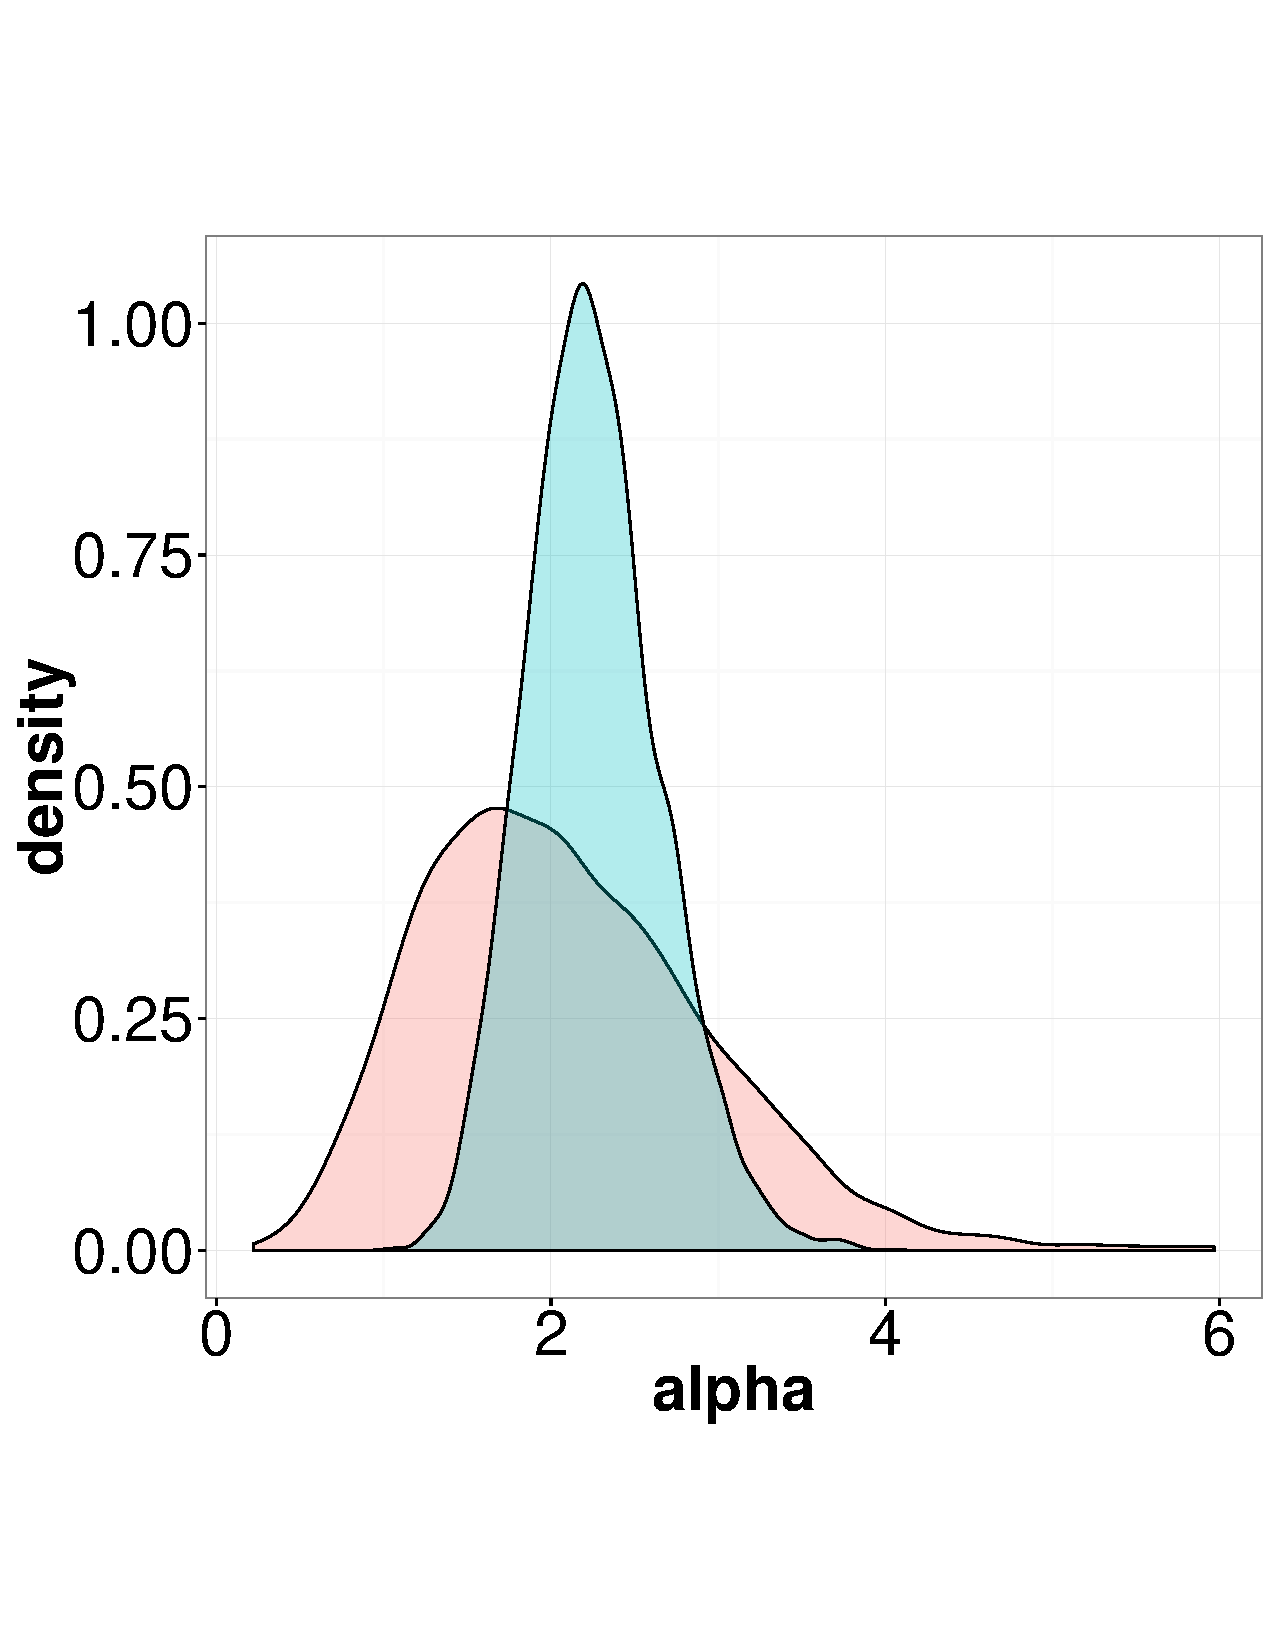
\includegraphics [width=0.90\textwidth, angle=0]{figs/dist_alpha.pdf}
%   \vspace{-0 in}
% \end{minipage}
% \begin{minipage}[!hp]{0.45\linewidth}
% \centering
%   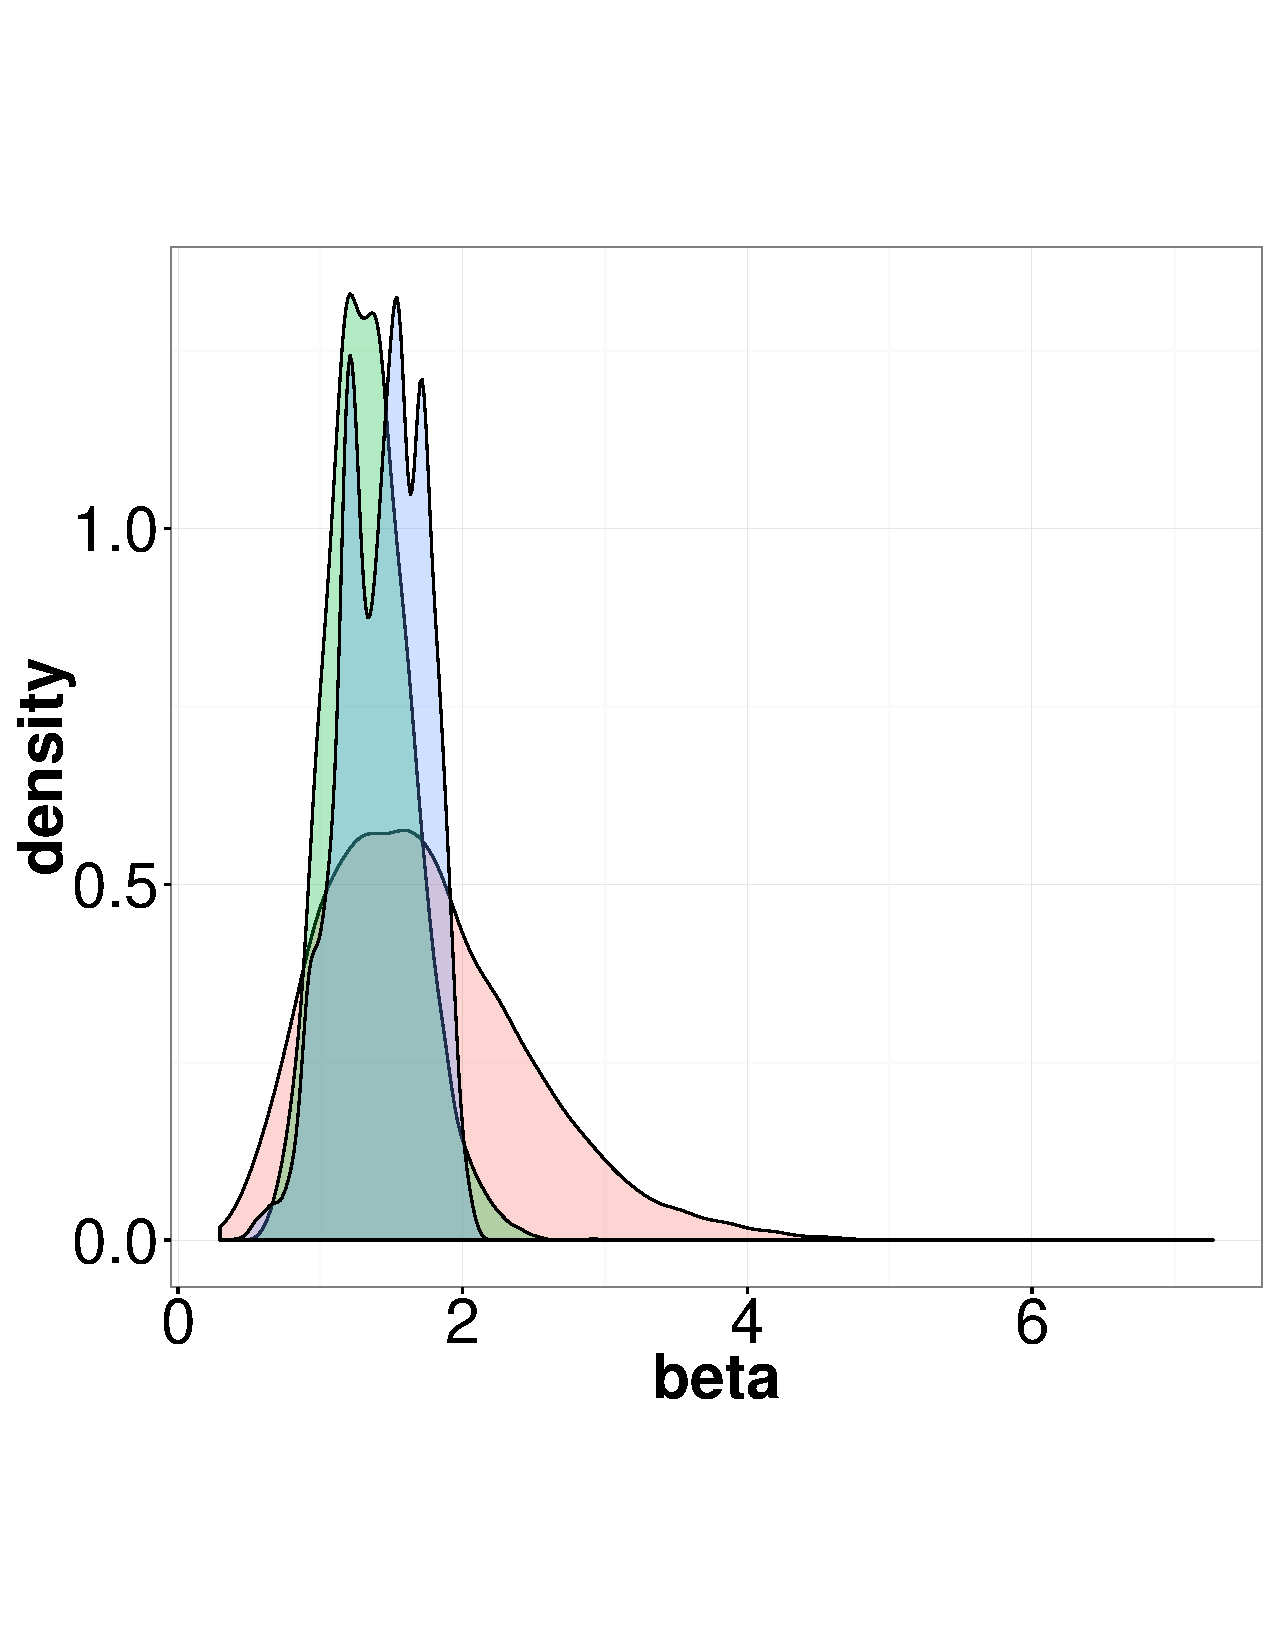
\includegraphics [width=0.90\textwidth, angle=0]{figs/dist_beta.pdf}
%   \vspace{-0 in}
% \end{minipage}
%   \caption{density.The left is for $\alpha$, and the right is for $\beta$.}
%    \label{fig:dist}
% \end{figure}
\subsubsection{A time-inhomogeneous immigration model}~
Here we extend the previous model to incorporate a known time-inhomogeneity. 
The arrival and death rates are no longer constant, and are instead given by
 %$$A_i(t) =: A_{i,i}(t) = -(\alpha + i\beta)w(t), \; \; i =0,1,...,N$$ 
$A_{i, i+1}(t) = \alpha w(t) \ (i =0,1,\cdots,N-1)$ respectively.
While it is not difficult to work with sophisticated choices of $w(t)$,
here we limit ourselves to a simple piecewise-constant choice of $w(t)$ 
given by $w(t) = \left\lfloor \frac{t}{5} \right\rfloor$. Even such a simple
change in the original model can dramatically affect the performance
of the Gibbs sampler.
% $w(t) = w_i, \; t \in [\l_i, l_{i + 1}), i = 1,2,3,..., K$.
%\noindent Assume: $S = [S_0,S_1, ...,S_N] \;, T = [t_0(t_{start}), t_1,...,t_N, 
%t_{N+1}(t_{end})]$, and y as observations.\\
%Now, let's consider a immigration model as follows. State space is 
% $\{0, 1, 2, ..., N - 1\}$, representing the total population. 
% We already know the conditional density(given $\alpha,\; \beta$) of a MJP trajectory $(s_0, S, T)$ in time interval $[t_{start}, t_{end}]$, with $S=(s_1, s_2,..., s_k)$, $T=(t_1, t_2,..., t_k)$. 
% $$f(s_0,S,T| \alpha, \beta) = \prod_{i=0}^{k-1} A_{s_i, s_{i+1}}(t_i) \exp(\sum_{i=0}^{k} A_{s_i}(t_i)(t_{i+1} - t_{i})), $$
% where $t_0 = t_{start}$, $t_{k+1} = t_{end}.$\\
% Let's denote some notations here.\\
% $$U(s_0, S, T):= \sum_{i=0}^{k-1} \mathbb{I}_{\{s_{i+1} - s_i = 1\}}.$$
% $$D(s_0, S, T):= \sum_{i=0}^{k-1} \mathbb{I}_{\{s_{i+1} - s_i = -1\}}.$$
% Call them U and D for short.
% Let's denote the total time when the trajectory state stays at state i as $\tau_i$, i.e. $\tau_i = \sum_{j=0}^{k} (t_{j+1} -t_j)\mathbb{I}_{\{s_j = i\}}$, then $\sum_{i=0}^k (t_{i+1} - t_i)s_i = \sum_{i=0}^N \tau_ii.$\\

% $$f(s_0,S,T| \alpha, \beta) \propto \exp(\sum_{r = 0}^{K}-w_r\alpha(l_{r + 1} - l_{r}- \tau_N^r) )\alpha^U \cdot  \exp(-\int_{t_s}^{t_{e}}(S(t)w(t)\beta)  \beta^D$$\\
% If we assume the prior of $\alpha$, and $\beta$ are $Gamma(\mu,\lambda)$, $Gamma(\omega, \theta)$, which are independent with each other. \\
% $$p(\alpha) = \frac{\lambda^\mu}{\Gamma(\mu)}\alpha^{\mu -1}e^{-\lambda \alpha}. $$
% $$p(\beta) = \frac{\theta^\omega}{\Gamma(\omega)}\beta^{\omega -1}e^{-\theta \beta}. $$
% Then we can get the posterior distribution $$f(\alpha, \beta | s_0,S,T)$$ as follows.
% $$ f(\alpha, \beta | s_0,S,T) \propto \exp(-(\lambda +\sum_{r = 0}^{K}w_r\alpha(l_{r + 1} - l_{r}- \tau_N^r))\alpha) \alpha^{\mu + U -1} \cdot \exp(-(\int_{t_{s}}^{t_{e}}(S(t)w(t) + \theta)\beta) \beta^{\omega+ D -1}.$$
% It means that the posterior distributions of $\alpha$, $\beta$ are still independent. \\
% $\alpha | s_0,S,T$ is following $Gamma(\mu+ U,\lambda +\sum_{r = 0}^{K}w_r\alpha(l_{r + 1} - l_{r}- \tau_N^r)  )$\\
% $\beta | s_0,S,T$ is following $Gamma(\omega+ D,\int_{t_s}^{t_{e}}(S(t)w(t) + \theta)$.\\
% Such immigration models have perfectly conjugate posterior distributions when we assign $\gamma$ priors to $\alpha$ and $\beta$. We apply our Metropolis Hasting algorithms on such models to compare the performance with the performance of Gibbs Sampling algorithm.

%\subsection{Experiments}

 The top row of figure~\ref{fig:ESS_pc_10} plots the ESS per unit time for the 
 parameters $\alpha$ (left) and $\beta$ (right) for the immigration model with 
 capacity $3$.  Now, the symmetrized MH algorithm is significantly 
 more efficient, comfortably outperforming all samplers (including the Gibbs 
 sampler) over a wide range of settings. %The Gibbs sampler slightly outperforms
 %the simple MH sampler, while particle MCMC is significantly worse (we have
% not included it).  
 Figure~\ref{fig:ESS_pc_10} shows performance for dimension
 $10$, once again the symmetrized MH-algorithm performans best over a 
 range of settings of the proposal variance. We note that increasing the
 dimensionality of the state space results in a more concentrated posterior,
 shifting the optimal setting of the proposal variance to smaller values.
  \begin{figure}%[b]
  \centering
  \begin{minipage}[!hp]{0.8\linewidth}
  \centering
    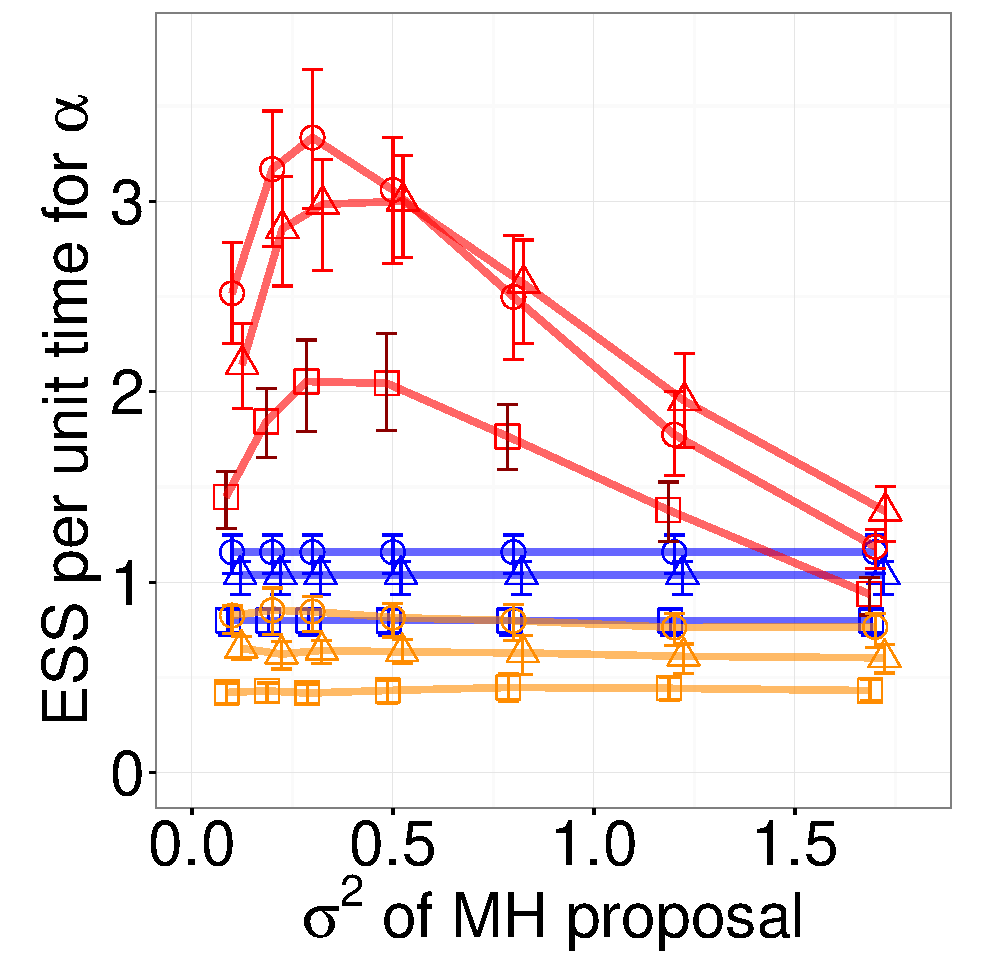
\includegraphics [width=0.48\textwidth, angle=0]{figures_new_apr12/CQ_alpha_dim3_18apr12.pdf}
    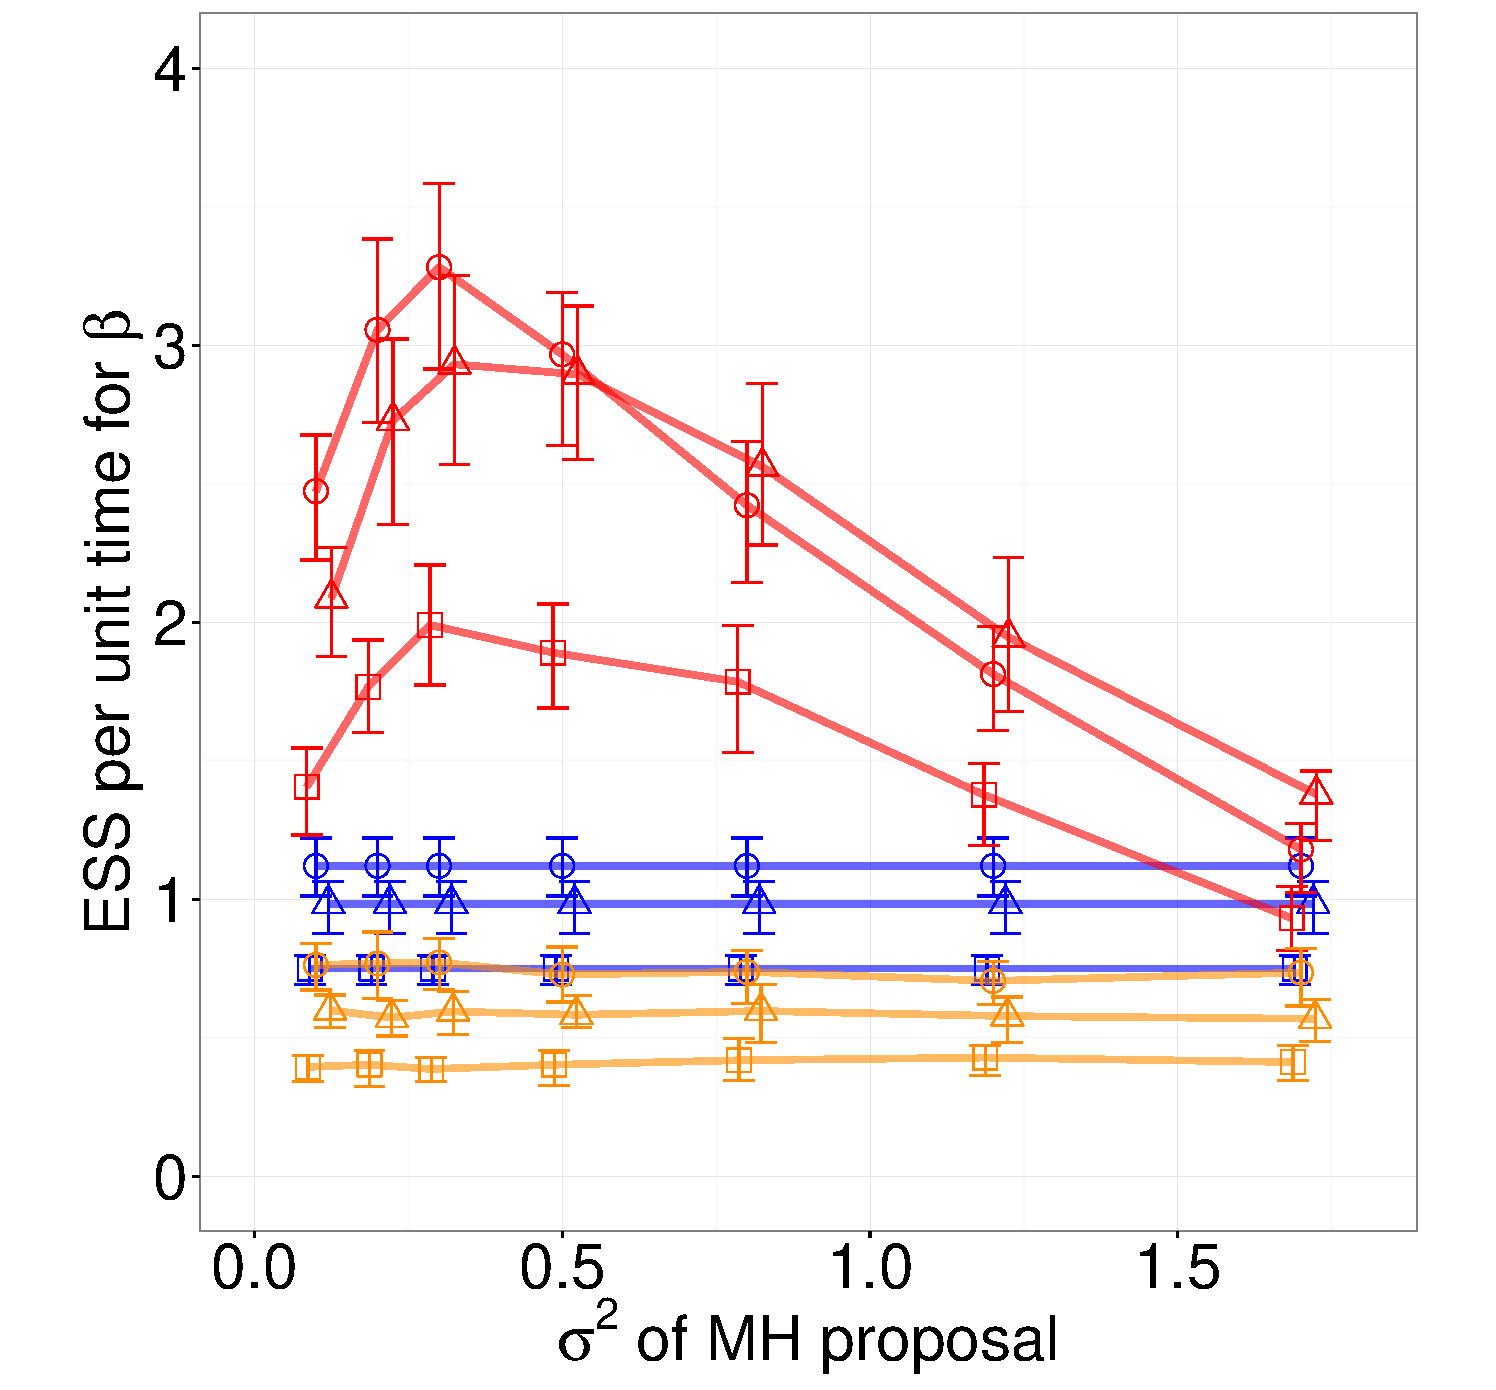
\includegraphics [width=0.48\textwidth, angle=0]{figures_new_apr12/CQ_beta_dim3_18apr12.pdf}
%    \vspace{-.81 in}
  \centering
    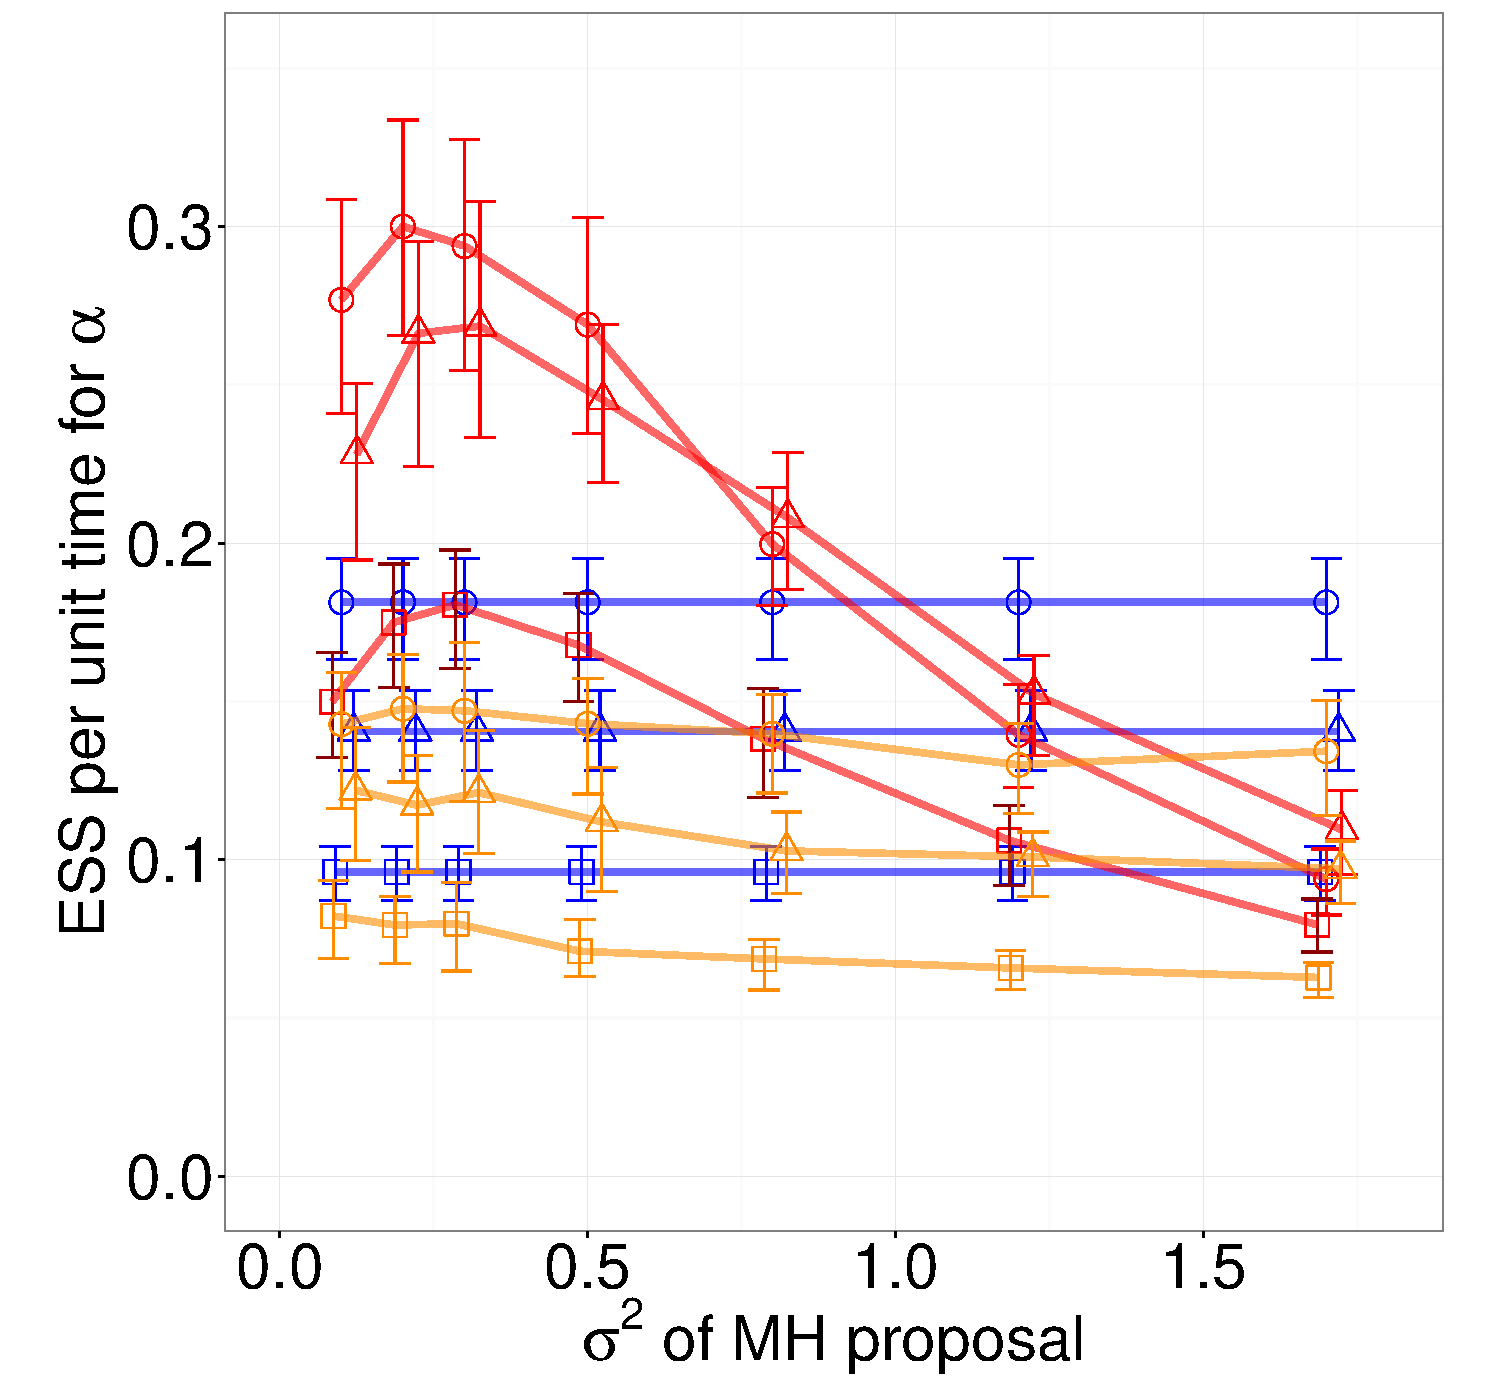
\includegraphics [width=0.480\textwidth, angle=0]{figures_new_apr12/CQ_alpha_dim10_18apr12.pdf}
    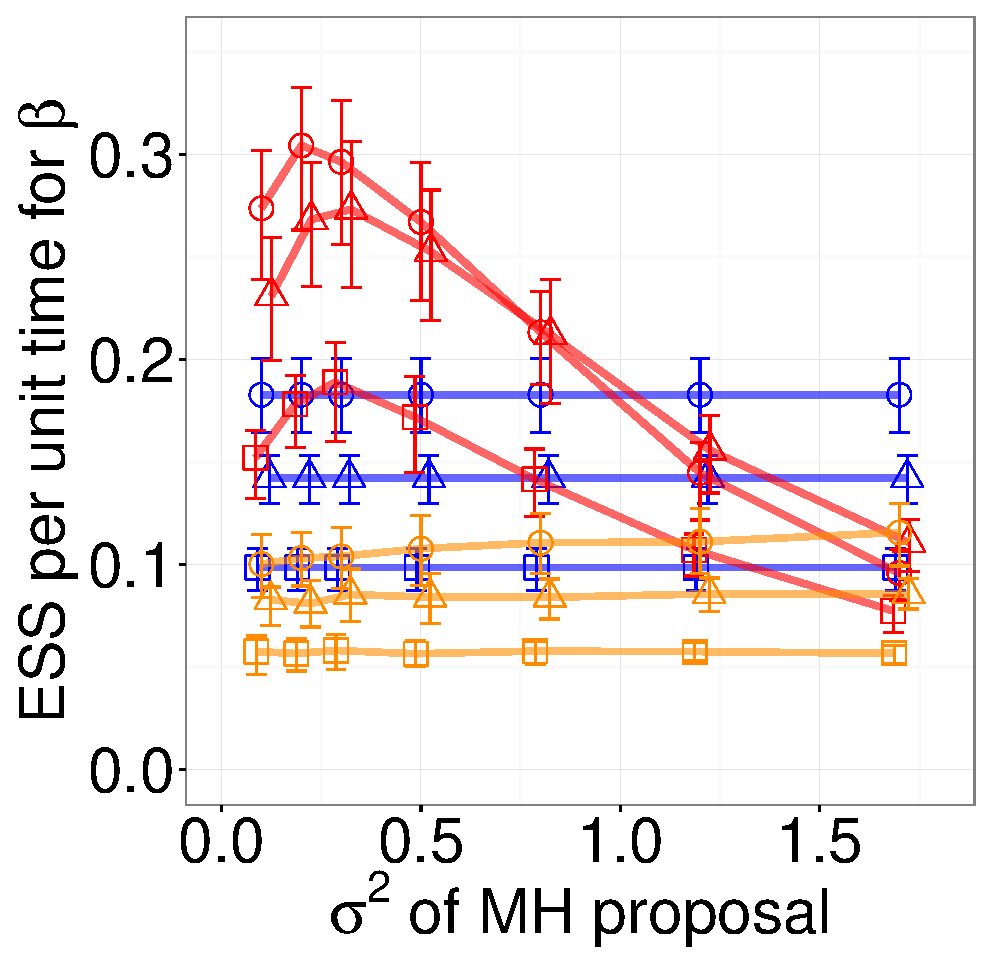
\includegraphics [width=0.480\textwidth, angle=0]{figures_new_apr12/CQ_beta_dim10_18apr12.pdf}
%    \vspace{-.5in}
  \end{minipage}
  \begin{minipage}[!hp]{0.19\linewidth}
    \caption{ESS/sec for the time-inhomogeneous immigration model, the top row 
      being dimension 3, and the bottom,
      dimension 10. The left column is for $\alpha$, and the 
    right is for $\beta$. Red, yellow and blue curves are the symmetrized MH,
  \naive\ MH, and Gibbs algorithm.}
     \label{fig:ESS_pc_10}
  \end{minipage}
  \end{figure}

  \subsection{Analysis of Chi site data for Escherichia coli}~
  We analyze the Escherichia coli data used in Fearhead. The data are for E. coli DNA and consist of the position (in bases) of Chi sites along the genome while the Chi site is a motif of eight base pairs: GCTGGTGG. The circular double-stranded DNA genome of E. coli has two strands which are the inner and outer rings. The molecular mechanisms of DNA replication differ between the two half-strands and they are termed leading and lagging. The E. coli genome is 4639675 bases long and each half is 2319.838 kilobases long. We model this discrete process as continuous process because of the length. Further, we model this using Markov-modulated Poisson process. Specifically, we analyze the inner lagging strand data by our Metropolis Hasting sampler compared with Gibbs sampler. A Markov-modulated Poisson process is a Poisson process whose intensity depends on the current hidden state of a continuous time Markov chain. Points from the Markov-modulated Poisson process are observed. We assume the hidden state space is  $\{1, 2\}$ and the corresponding Poisson-rates are $\lambda_1$ and $\lambda_2$. Transitions from state $1$ to state $2$ have rate $\alpha$ while transitions from state $2$ to state $1$ have rate $\beta$. Gamma priors are placed for these four parameters. Specifically, we use Gamma$(2,2)$, Gamma$(2,3)$, Gamma$(3,2)$, Gamma$(1,2)$ for $\alpha$, $\beta$, $\lambda_1$, $\lambda_2$ respectively.
  \begin{figure}%[b]
  \centering
  \begin{minipage}[!hp]{0.99\linewidth}
  \centering
    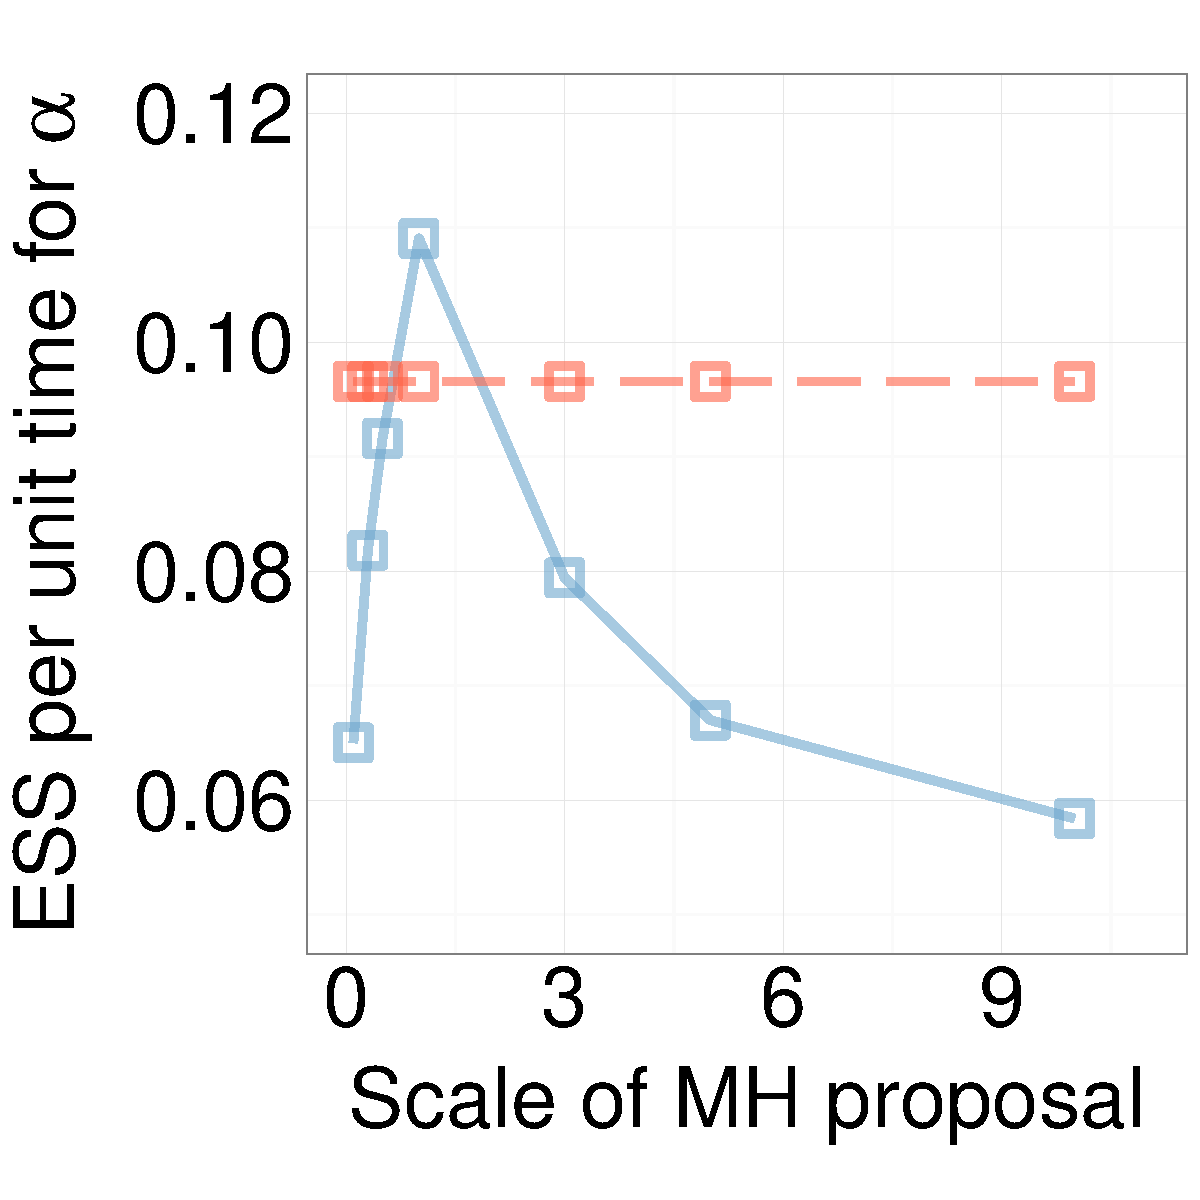
\includegraphics [width=0.33\textwidth, angle=0]{figs/ECOLI_alpha.pdf}
    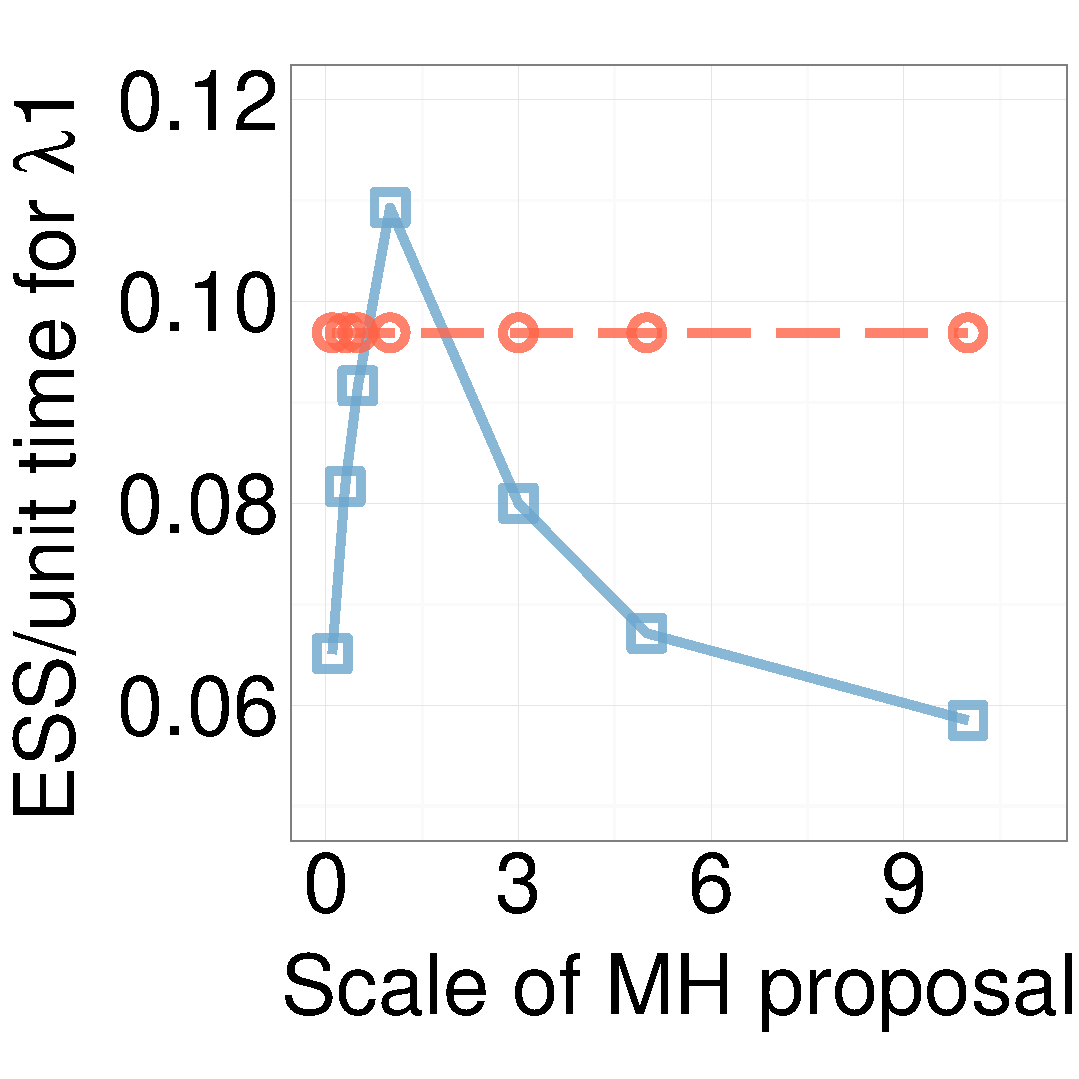
\includegraphics [width=0.33\textwidth, angle=0]{figs/ECOLI_l1.pdf}
%    \vspace{-.81 in}
 %   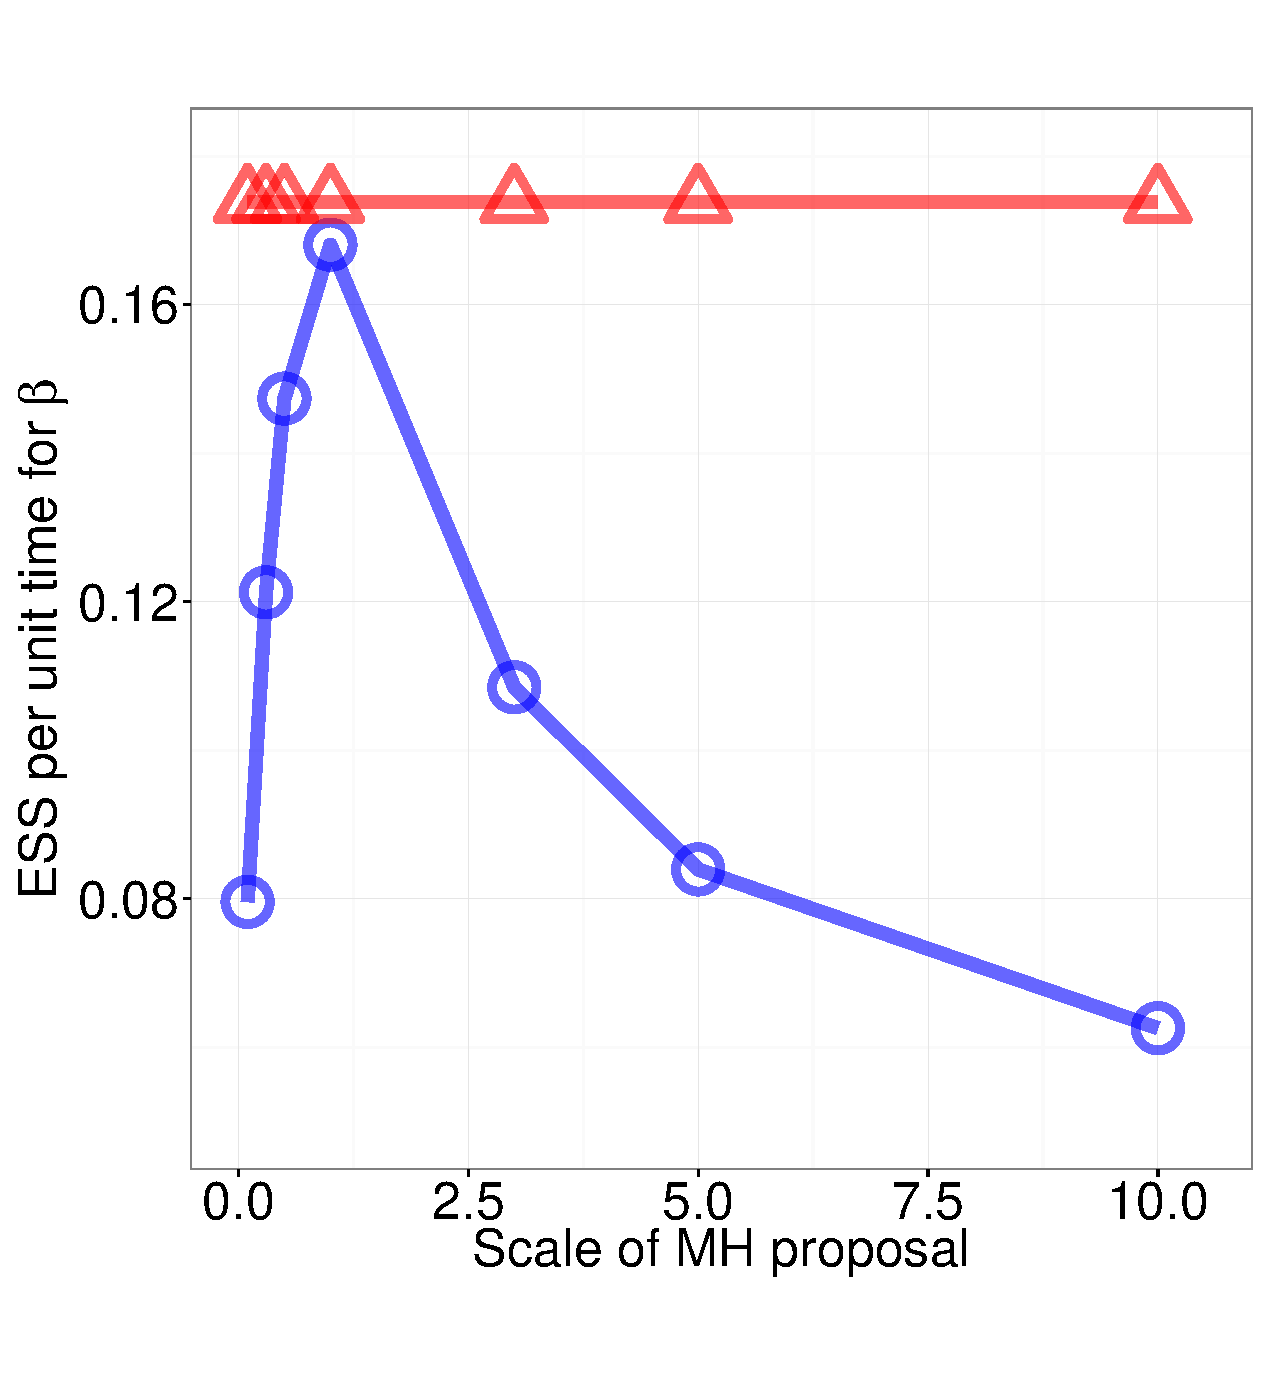
\includegraphics [width=0.24\textwidth, angle=0]{figs/ECOLI_beta.pdf}
 %  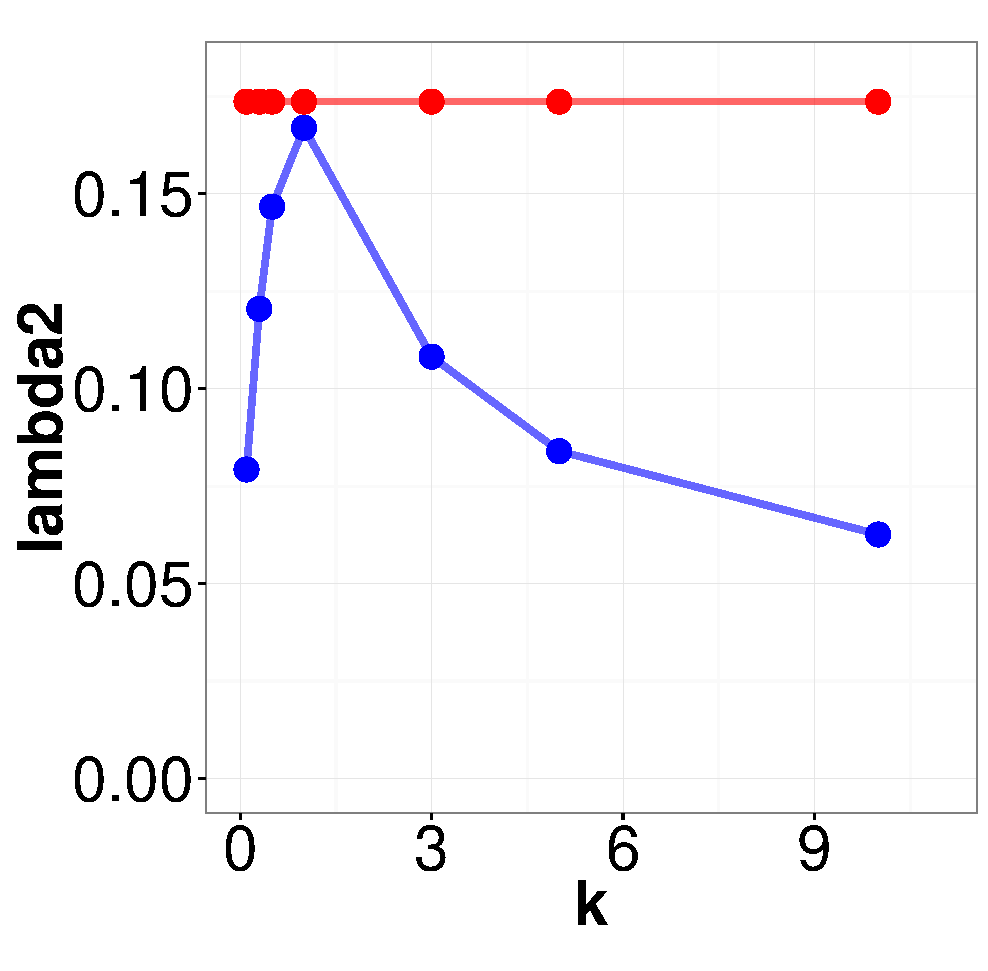
\includegraphics [width=0.24\textwidth, angle=0]{figs/ECOLI_l2.pdf}
  %  \vspace{-.5in}
  \end{minipage}
    \vspace{-.2in}
    \caption{ESS/sec for the EColi data.}
     \label{fig:ECOLI}
  \end{figure}



\section{Geometrical ergodicity of the MH algorithm}~
As shown before, virtual jumps are sampled after uniformization procedure. Let's consider the redundant representation of the trajectory. $V = (v_0, v_1, v_2,..., v_n)$, $W = (w_1, w_2, w_3,..., w_n)$, where $v_i$ can be the same as $v_{i + 1}$. Denote $X$ as $(W, V, \theta)$. Also assume that noisy observations $Y = (Y_1, Y_2, ..., Y_k)$ are observed at some determined times $(t_1^{obs}, t_2^{obs}, ..., t_k^{obs})$. We will show that the chain of $X's$ is geometrically ergodic. Let $P$ be the transition kernel of the Markov chain $X_n$ generated by Algorithm 1. Let $\Pi(X)$ be the target distribution, which is the posterior distribution $P(X | Y)$. First, consider the following posterior distribution.
\begin{align*}
P(V | W, Y, \theta) &\propto  P(W, V | \theta) P(Y | W, V) p_0(\theta)\\
&= \nu_0(v_0)g_0(v_0; \theta)\prod_{i = 1}^n P(v_{i - 1}, v_i; \theta)g_i(v_i; \theta) p_0(\theta)\\
\end{align*}
\begin{align*}
g_i(v; \theta) &= \Omega(\theta) \exp(-(w_{i + 1} - w_i)\Omega(\theta)) \prod_{j: w_i < t_j^{obs} < w_{i + 1}} L_j(Y_j| v)\\
g_n(v; \theta) &= \exp(-(t_{end} - w_n)\Omega(\theta)) \prod_{j: w_n < t_j^{obs} < t_{end}} L_j(Y_j| v)\\
\end{align*}
Given the jumping times $W$, the state on the jumping times is a discrete time markov chain with $B(\theta)$ as transition matrix.
\begin{align*}
B(\theta) = I + \frac{A(\theta)}{\Omega(\theta)}\\
\end{align*}
The following is $n_0$ step transition probability.
\begin{align*}
B_{i - n_0 : i}(v_{i - n_0}, s_i = v; \theta) = \sum_{v_{i - n_0 + 1}, v_{i - n_0 + 2},...,v_{i - 1}} (\prod_{l = i - n_0 + 1}^{i - 1} B(v_{l - 1}, v_l; \theta))B(v_{i - 1}, v; \theta)\\
B_{i - n_0 : i}^{g}(v_{i - n_0}, s_i = v; \theta) = \sum_{v_{i - n_0 + 1}, v_{i - n_0 + 2},...,v_{i - 1}} (\prod_{l = i - n_0 + 1}^{i - 1} B(v_{l - 1}, v_l; \theta)g_l(v_l; \theta))B(v_{i - 1}, v; \theta)\\
\end{align*}
\begin{theorem}~
  Denote the state space as $S$ and the parameter space as $\Theta$, and assume that:\\
1. Exist an irreducible rate matrix $A^{min}$ such that $A(s, s';\theta) \geq A^{min}(s, s')$, for $\forall s \in S$ and $s' \in S$, where $s \neq s'$.\\
2. For $\forall \theta$, $\forall s$,  and the determined $\Omega(\theta)$, there exits an $\eta$ such that $\frac{A(s; \theta)}{\Omega(\theta)} \leq 1 - \eta$, where $A(s; \theta) = \sum_{s' \neq s} A(s, s';\theta)$.\\
3. $\exists \Omega^{max} < +\infty$, such that, $\forall \theta$, $\Omega(\theta) \leq \Omega^{max}$.\\
4. $\exists \kappa > 0$ such that the proposal distribution in MH step $q(\theta' | \theta) \geq \kappa q_0(\theta_0)$, where $q_0(\theta_0)$ is the prior distribution of $\theta$.\\
\indent Then the chain $X_n$ generated by Algorithm 1 is geometrically ergodic, i.e. there exist an constant $\gamma$ and a function $M(X)$ such that $L(Y | X) > 0$ and every m, $$\Vert P^m(X, \cdot) - \Pi(\cdot) \Vert_{tv} \leq \gamma^m M(X).$$
\end{theorem} 
\begin{lemma}~
   For a fixed $n_0$ , and $\forall$ $i$  such that $ n_0 \geq i \leq n - 1$, assume that\\
1. $\exists$  $ \xi > 0$, $B_{i - n_0: i}(v_{i - n_0}, v; \theta) \geq \xi$, $\forall$ $v_{i - n_0}, v \in S$.\\
2. $\exists$  $\eta > 0$, $B(v,v ; \theta) \geq \eta$, $\forall$, $v \in S$.\\
3. $\exists$  $g_l^{min} > 0$, $g_l^{max}$, such that $g_l^{min} \leq g_l(v; \theta) \leq g_l^{max}$, for $\forall$ $v \in S$, and $\forall$ $l \in [i - n_0 + 1, i]$\\ 
Then $\mathbb{P}(V_i = v | V_{i + 1} = v, W, \theta, Y) \geq \delta_i$ and $\delta_i = \xi\eta \prod_{l = i - n_0 + 1}^i \frac{g_l^{min}}{g_l^{max}}$.
\end{lemma}
\begin{proof}
  We condition on $V_{i - n_0} = v_{i - n_0}$ and we can get the following. 
\begin{align*}
\mathbb{P}(V_i = v | v_{i + 1} = v, V_{i - n_0} = v_{i - n_0} W, \theta, Y) &= \frac{\mathbb{P}(V_i = v | v_{i - 1} = v, V_{i - n_0}| W \theta, Y)}{\mathbb{P}(v_{i + 1} = v, V_{i - n_0}| W \theta, Y)} \\
&= \frac{B_{i - n_0: i}^g(v_{i - n_0}, v; \theta)g_i(v;\theta)B(v,v;\theta)}{\sum_{v'}B_{i - n_0: i}^g(v_{i - n_0}, v'; \theta)g_i(v';\theta)B(v',v;\theta)} \\
&\geq \frac{\prod_{l = i - n_0 + 1}^i g_l^{min}}{\prod_{l = i - n_0 + 1}^i g_l^{max}} \frac{B_{i - n_0: i}(v_{i - n_0}, v; \theta)B(v, v; \theta)}{\sum_{v'}B_{i - n_0: i}(v_{i - n_0}, v'; \theta)B(v', v; \theta)}\\
&\geq \xi \eta \prod_{l = i - n_0 + 1}^i \frac{g_l^{min}}{g_l^{max}}
\end{align*}
\end{proof}
\begin{lemma}~
 If the assumptions of Lemma 2 hold for $\forall$ $i \in [n_0, n - 1]$, then $\mathbb{E}[|J| | W, \theta, Y] \leq |W|  + 1- \sum_{i = n_0}^{|W| - 1} \delta_i$, where $J = \{i \in [1, n]: V_i \neq V_{i - 1}\} \cup \{ 0 \}$ for $\forall \theta \in \Theta$.
\end{lemma}
\begin{proof}
We notice that $|W| = n$. Apply lemma 2 to every $i \in [n_0, n - 1]$. We can get $\mathbb{P}(V_i = v| V_{i + 1}, W, \theta, Y) \geq \delta_i.$ Then $\mathbb{E} \mathbb{I}_{\{V_i \neq V_{i + 1} \}} = \mathbb{E}[\mathbb{P}(V_i \neq V_{i + 1}| V_{i + 1}, W, \theta, Y) | W, \theta, Y] \leq 1 - \delta_i$. Then we apply the naive upper bound $1$ for every $i < n_0$. Then $$\mathbb{E}[|J| | W, \theta, Y] = \mathbb{E}[1 + \sum_{i = 0}^{n - 1}\mathbb{I}_{\{V_i \neq V_{i + 1}\}}| W, \theta, Y] \leq n + 1 - \sum_{i = n_0} ^ {n - 1} \delta_i.$$
\end{proof}
\begin{proposition}
  (Drift Condition)  Under the assumptions of theorem 1, there exit   $0 < \delta < 1$ and $c < +\infty$ such that in one step of algorithm 1, $\mathbb{E} [|J(X')| |X] \leq (1 - \delta) |J(X)| + c$.
\end{proposition}
\begin{proof}
Assume the current state is $X = (V, W, \theta)$, where $V = (v_0, v_1, v_2,..., v_n)$, $W = (w_1, w_2, w_3,..., w_n)$. First we will show there exists a $n_0$, such that the assumptions of lemma 2 hold for this $n_0$. Let $B^{min} = I + \frac{A^{min}}{r^{max}}$. Because $A^{min}$ is irreducible, $B^{min}$ is irreducible too. So there exists $n_0 \in \mathbb{Z}^+$ and $\xi > 0$ such that $(B^{min})^{n_0}(v, v') \geq \xi$ for $\forall v, v' \in S$. So condition 1 of lemma 2 holds. Assumption 2 of Theorem 1 leads to condition 2 of lemma 2. \\
In the first step of algorithm 1, virtual jumps $U$ are sampled. And we get $W'$. $|U|$ is poisson distributed with rate $\int_{t_{start}}^{t_{end}}(\Omega(\theta) - A(X_t))dt \leq \Omega^{max}(t_{end} - t_{start})$. So $\mathbb{E}[|W'| | X] \leq |J(X)| + \Omega^{max}(t_{end} - t_{start})$.\\For condition 3 of lemma 2, the upper bound is uniform for all $l$. $g_l^{max} = \Omega^{max}$. For the lower bound, if $g_l(v; 
\theta)$ includes likelihood factors, then we simply use $0$ as lower bound. For the remaining, we have a uniform lower bound $g_l^{min} = \Omega^{min} \exp(\Omega^{max}(t_{end} - t_{start}))$, where $\Omega^{min} = \min_{v}\{ \sum_{v' \neq v} A(v, v')\}$. There are at most $k$  $g_l(v; \theta)$ which contains likelihood factors. If $g_l^{min} = 0$, then let $\delta_i = 0$ for $i \in [l, l + n_0 - 1]$. We also let $\delta_i = 0$ for $ i < n_0$. So there are at most $(k + 1) n_0$ indices $i$ such that $\delta_i = 0$. For at least $n - (k + 1)n_0$ indices such that $\delta_i = \xi \eta (\frac{g^{min}}{g^{max}})^{n_0} \triangleq \delta$ which is free of $\theta$.\\ 
Then apply lemma 3 using the $\delta_i$ we define earlier. $\mathbb{E}[|J'| W', \theta', Y] \leq |W'| + 1 - (|W'| - (k + 1) n_0) \delta \leq (1 - \delta) |W'| + ((k + 1)n_0\delta + 1)$\\
$$\mathbb{E}[J(X') | X] = \mathbb{E}[\mathbb{E}[J(X')| W'] | X] \leq (1- \delta)(|J(X)| + \Omega^{max}(t_{end} - t_{start})) + (k + 1)n_0\delta + 1.$$
\end{proof}
\begin{proposition}
  (Small set Condition)  The set $\{ X: |J(X)| \leq h \}$ is 1-small for every $h > 0$. I.e. there exits a probability measure $\Psi$ and a constant $\beta > 0$ such that $P(X, dX') \geq \beta \Psi(dX')$, where $|J(X)| \leq h$.
\end{proposition}
\begin{proof}
First choose a $V^\dagger = (v_1^\dagger, v_2^\dagger,..., v_k^\dagger)$ such that $\prod_{j = 1}^k L_j(Y_j|v_j^\dagger) \triangleq L^\dagger > 0$. Then define $V^\ast = (v_0^ \ast, v_1^\ast, ...,v_m^\ast)$ such that $V^\dagger$ is a sub-sequence of $V^\ast$, where $v_i^\ast \neq v_{i + 1}$. Also, embed $t^{obs} = (t_1^{obs}, t_2^{obs},..., t_k^{obs})$ in a longer time sequence $W^\ast = (w_1^\ast, w_2^\ast,...,w_m^\ast)$.\\
$$\nu_0(v_0^\ast) \prod_{i = 1} ^ {m - 1}B(v_i^\ast,v_{i + 1}^\ast; \theta) \geq \nu_0(v_0^\ast) \prod_{i = 1} ^ {m - 1} \frac{A^{min}(v_i^\ast,v_{i + 1}^\ast)}{\Omega^{max}} \triangleq \beta_2^\ast.$$
Define the regeneration measure $\Psi(dX')$ as follows.\\
$$W_i' \sim Unif(w_{i - 1}^\ast, w_i^\ast)$$ 
$$V_i' = v_i$$
$$\theta' \sim p_0(\cdot)$$
The random vector $(w_1', w_2',...,w_m')$ has the uniform distribution on the set $\tau = \{ (w_1, w_2,...,w_m)|w_{i - 1}^\ast \leq w_i\leq w_i^\ast\}$. There is another way in which algorithm 1 can be executed. $\Omega(\theta) - B(v; \theta) \geq \eta \Omega(\theta) \geq \eta \Omega^{min} \triangleq \epsilon$. In step 1, we independently sample two Poisson processes $U_0$ and $U_1$ with rates $\epsilon$ and $\Omega(\theta) - B(V_t; \theta)$. Let $U = U_0 \bigcup U_1$. Then $W' = J(X) \bigcup U$. $$\mathbb{P}(U_0 \in \tau) \triangleq \beta_0 > 0.$$
$$\mathbb{P}(U_1 = \varnothing) \geq \exp(-\Omega^{max}(t_{end} - t_{start})) \triangleq \beta_1 > 0.$$
In step 2 of algorithm 1, $\theta$ is updated under Metropolis Hasting scheme. First, $\theta'$ is proposed via the proposal kernel $q(\theta'| \theta)$, then $\theta'$ is accepted with probability $\alpha = 1 \wedge \frac{q(\theta | \theta')P(\theta'| W', Y)}{q(\theta' | \theta)P(\theta| W', Y)} \triangleq 1 \wedge \bar{\alpha}$. Assume $P(Y | V, W) \in [L_{min}, L_{max}]$
\begin{align*}
P(\theta, W', Y) &= \int p(V', \theta, W', Y) dV'\\
&= \int p_0(\theta)P(W, V | \theta)P(Y | V', W') dV'\\
&\in [L_{min}p_0(\theta)P(W'| \theta), L_{max}p_0(\theta)P(W'| \theta)]
\end{align*} 
We notice that $P(W' | \theta) = \Omega(\theta)^{|W'|}(t_{end} - t_{start})^{|W'|}\exp(-\Omega(\theta)(t_{end} - t_{start}))$
\begin{align*}
\bar{\alpha} &\geq \frac{q(\theta | \theta' )}{q(\theta' | \theta)} \frac{L_{min}}{L_{max}}\frac{P(W' | \theta')}{P(W'|\theta)}\frac{p_0(\theta)}{p_0(\theta)}\\
&\geq \frac{q(\theta| \theta')}{q(\theta' | \theta)}\frac{L_{min}}{L_{max}}(\frac{\Omega^{min}}{\Omega^{max}})^{|W'|}\exp(-\Omega^{max}(t_{end} - t_{start}))\frac{p_0(\theta')}{p_0(\theta)}\\
&\geq \kappa\frac{L_{min}}{L_{max}}(\frac{\Omega^{min}}{\Omega^{max}})^{|W'|}\exp(-\Omega^{max}(t_{end} - t_{start}))\frac{p_0(\theta')}{q(\theta' | \theta)}\\
&\triangleq \kappa C(|W'|)\frac{p_0(\theta')}{q(\theta' | \theta)}
\end{align*}
So for $\forall \theta' \in \Theta$, and given $W'$,
 \begin{align*}
&q(\theta' | \theta) \hat{\alpha} d\theta' \geq \kappa C(|W'|) p_0(\theta')d\theta'\\
&q(\theta' | \theta)  d\theta' \geq \kappa p_0(\theta')d\theta'\\
\end{align*}
So for $\forall \theta' \in \Theta$,  $\exists D(|W'|) = 1 \wedge C(|W'|) < +\infty$ such that $q(\theta' | \theta)\alpha d\theta' \geq D(|W'|)p_0(\theta')d\theta'$. We notice that $D(x)$ is decreasing with respect to $x$.\\
In step 2, FFBS is applied to sample a new trajectory given the jump times. We can use rejection sampling to do the same sampling $ V$ from $P(\cdot| W', \theta', Y)$ as follows.\\
(i) Simulate $V'$ with transition matrix $B(\cdot,\cdot;\theta')$ and initial distribution $\mu_0$.\\
(ii) Accept it with probability $\alpha= \frac{\mu_0(v_0')\prod_{i = 0}^{|W'| - 1}B(v_i', v_{i + 1}'; \theta)\prod_{i =0}^{|W'|}g_i(v_i'; \theta)}{\mu_0(v_0')\prod_{i = 0}^{|W'| - 1}B(v_i', v_{i + 1}';\theta) (\Omega(\theta))^{|W'| + 1}L_{max}} \geq \frac{(\Omega^{min})^{|W'| + 1}}{(\Omega^{max})^{|W'| + 1}L_{max}}$.\\
Suppose the current state is $X = (W, V, \theta)$ with $|J(X)| \leq h$ and the next state is $X' = (W', V', \theta)$. We define the following events\\
$(E_1)$: In step 1, we get $W' = J(X) \bigcup U_0$, and $U_0 \in \tau$. So $\mathbb{P}(E_1) \geq \beta_0 \beta_1 > 0$.\\
$(E_2)$: In step 2, we propose $\theta'$ and accept it. $\mathbb{P}(E_2) \geq D(m + h)p_0(\theta')d\theta'\triangleq \beta_2 p_0(\theta')d\theta'$, where $\beta_2 > 0$. \\
$(E_3)$: In step 3, all the jump times in $J(X)$ become virtual jump times. $\mathbb{P}(E_3) \geq \beta_2^\ast \eta^{|J(X)|} \geq \beta_2^\ast \eta^h \triangleq \beta_3 > 0$\\
$(E_4)$: given $E1$ -- $E3$, $V'$ is accepted. $\mathbb{P}(E_4) \geq (\frac{\Omega^{min}}{\Omega^{max}})^{m + h}\exp(-\Omega^{max}(t_{end} - t_{start})) \frac{L^\dagger}{L_{max}} \triangleq \beta_4$.\\
If $E_1$ -- $E_4$ happen, then a new trajectory $(W', V')$ is generated. It is independent with $X$. $p(W', V') = \Psi |_{(W,V)}(W', V')$.
So, $P(X, dX') \geq \beta_0\beta_1\beta_2\beta_3\beta_4 \Psi(dX')$.
\end{proof}
Theorem 1 directly follows from Propositions 4 and 5, according to Roberts and Rosenthal (2004).




\bigskip
%\begin{center}
%{\large\bf SUPPLEMENTAL MATERIALS}
%\end{center}

%\begin{description}

%\item[Title:] Brief description. (file type)

%\item[R-package for  MYNEW routine:] R-package �MYNEW� containing code to perform the diagnostic methods described in the article. The package also contains all datasets used as examples in the article. (GNU zipped tar file)

%\item[HIV data set:] Data set used in the illustration of MYNEW method in Section~ 3.2. (.txt file)

%\end{description}

~\nocite{RaoTeh13}
~\nocite{RaoTeh12}
~\nocite{Andrieu10}
~\nocite{Andrieu09}
~\nocite{Golightly15}
~\nocite{Andrieu102}
~\nocite{Liu94}
~\nocite{Neal12}
~\nocite{Neal03}
~\nocite{geoergo}
\bibliography{bibfile}
\bibliographystyle{plain}

\section{Supplementary material}

\subsection{Synthetic MJP}

  \begin{figure}[H]
  \centering
  \begin{minipage}[hp]{0.45\linewidth}
  \centering
    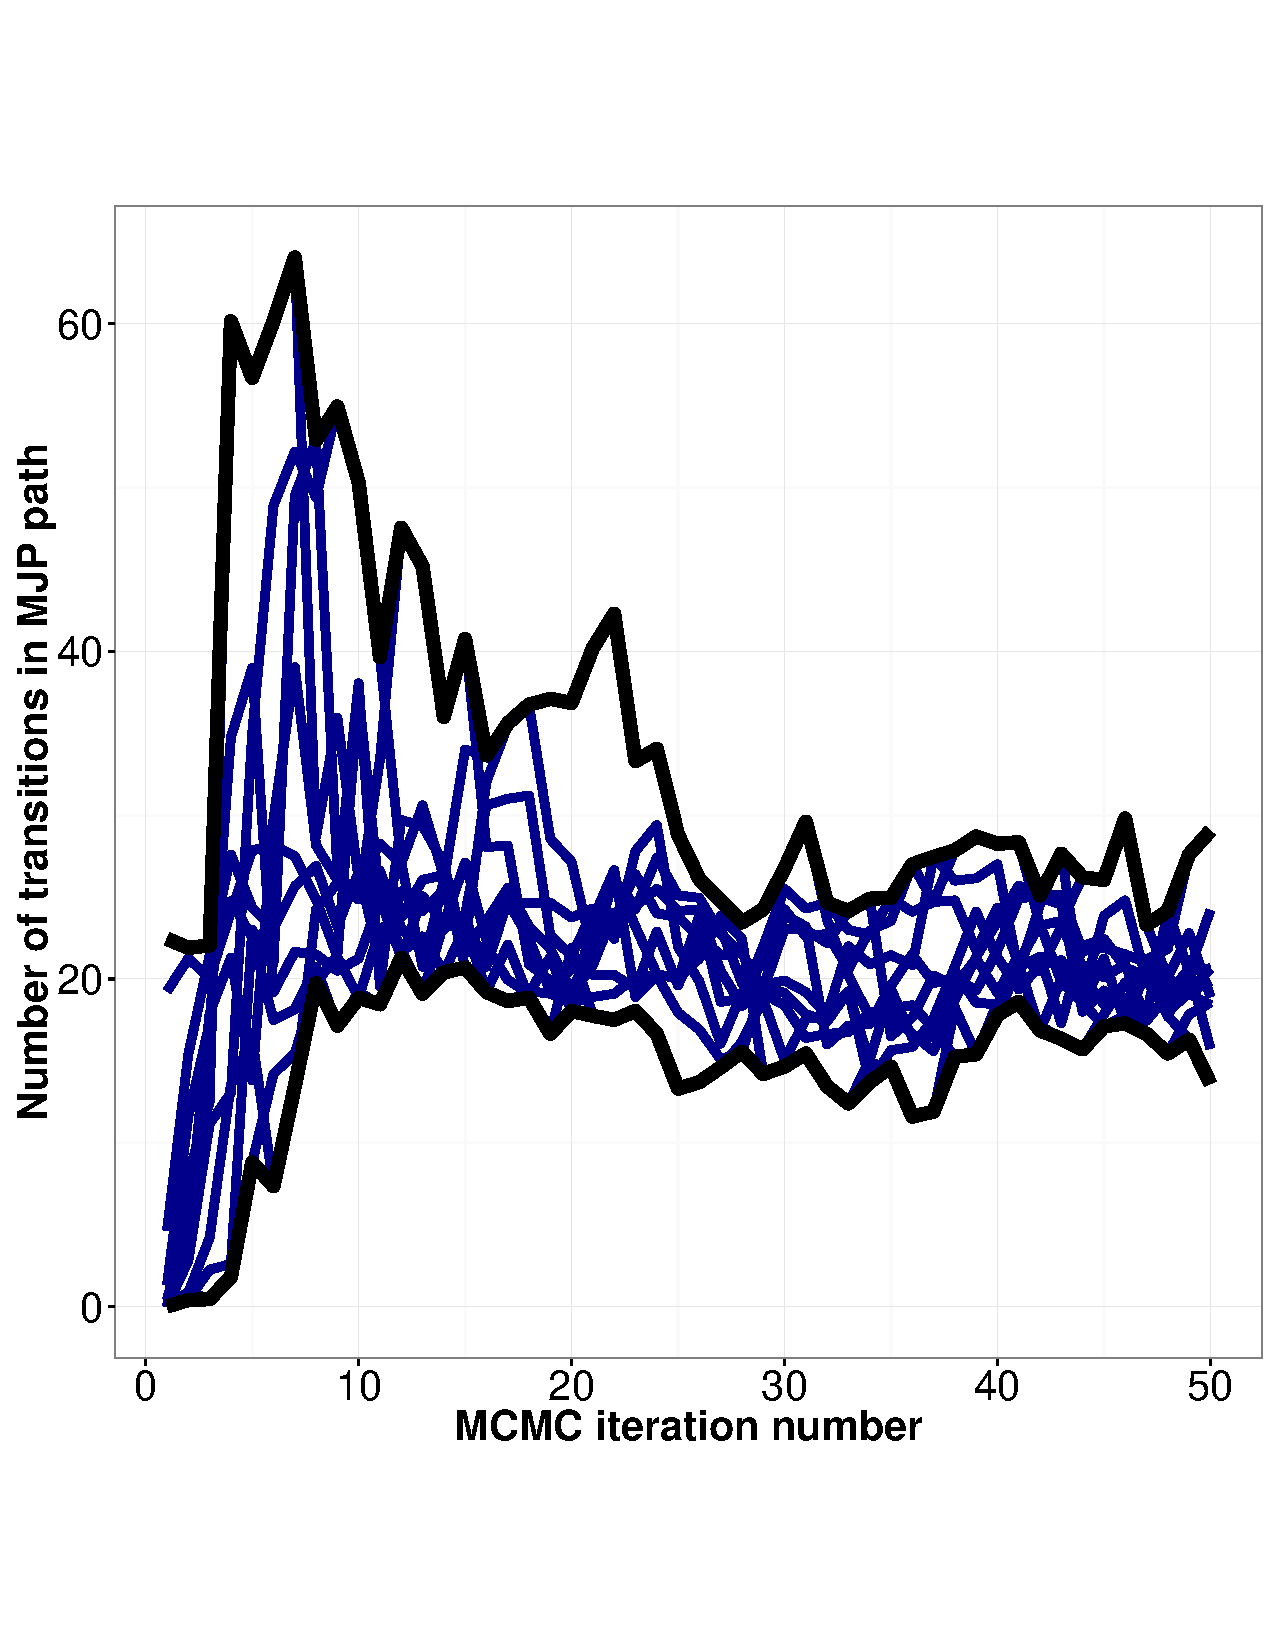
\includegraphics [width=0.90\textwidth, angle=0]{figs/exp3_k2_path_transition.pdf}
      \end{minipage}
    \caption{Trace plot of the number of MJP transitions for different initializatoins.}
	\label{fig:Transition_exp}
  \end{figure}

Figure~\ref{fig:Transition_exp} shows the initial burn-in of our improved MH 
sampler for the immigration-death model for different initializations. The vertical 
axis shows the number of state transitions in the MJP trajectory of each iteration. 
This quantity quickly reaches its equilibrium value within a few iterations.\\

% \begin{figure}[H]
% \centering
% \begin{minipage}[hp]{0.45\linewidth}
% \centering
%   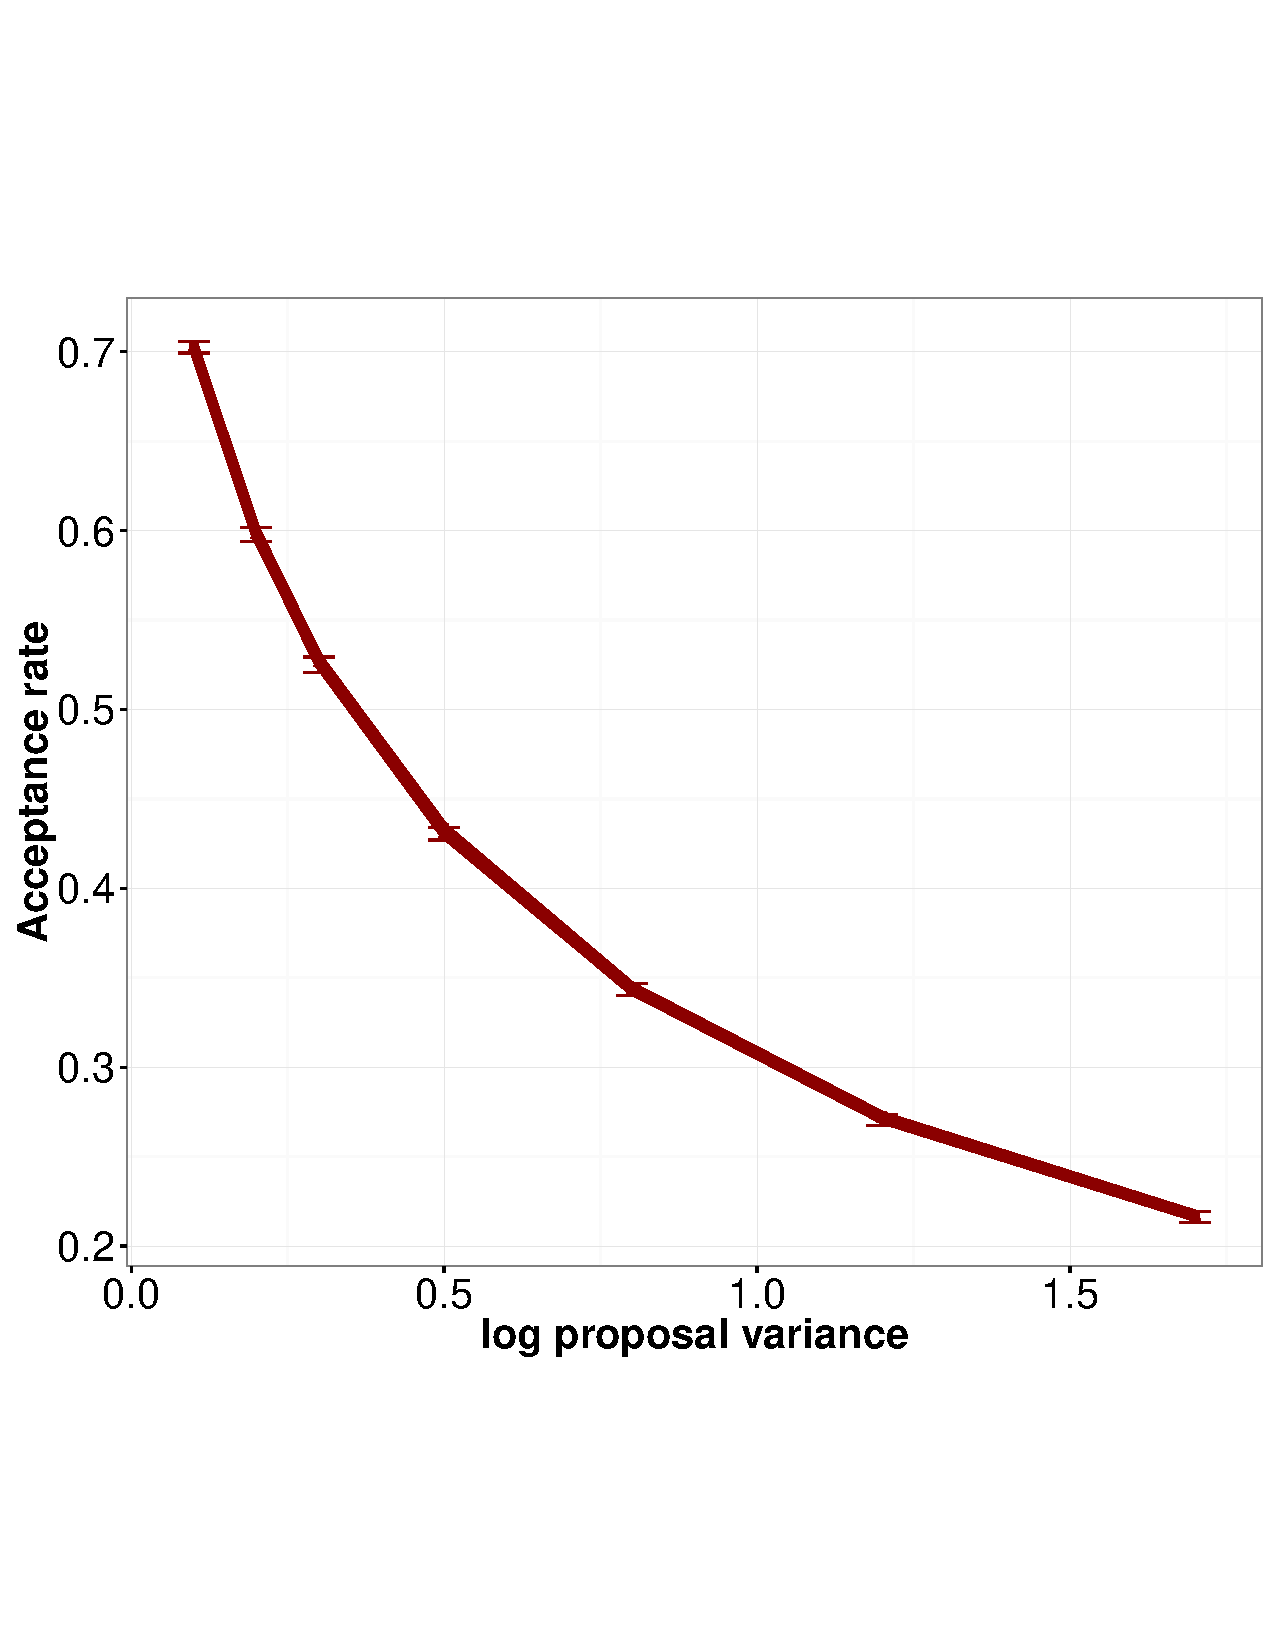
\includegraphics [width=0.90\textwidth, angle=0]{figs/acc_rate_exp_d3.pdf}
%     \end{minipage}
%   \caption{Acceptance rate for exp model (dim 3)}
%   \label{fig:acc_exp}
% \end{figure}

% Figure~\ref{fig:acc_exp} plots ESS plots the overall  acceptance rate against 
% the log variance of the proposal kernel per run for dimension $3$. 



  
    \begin{figure}[H]
  \centering
  \begin{minipage}[hp]{0.45\linewidth}
  \centering
    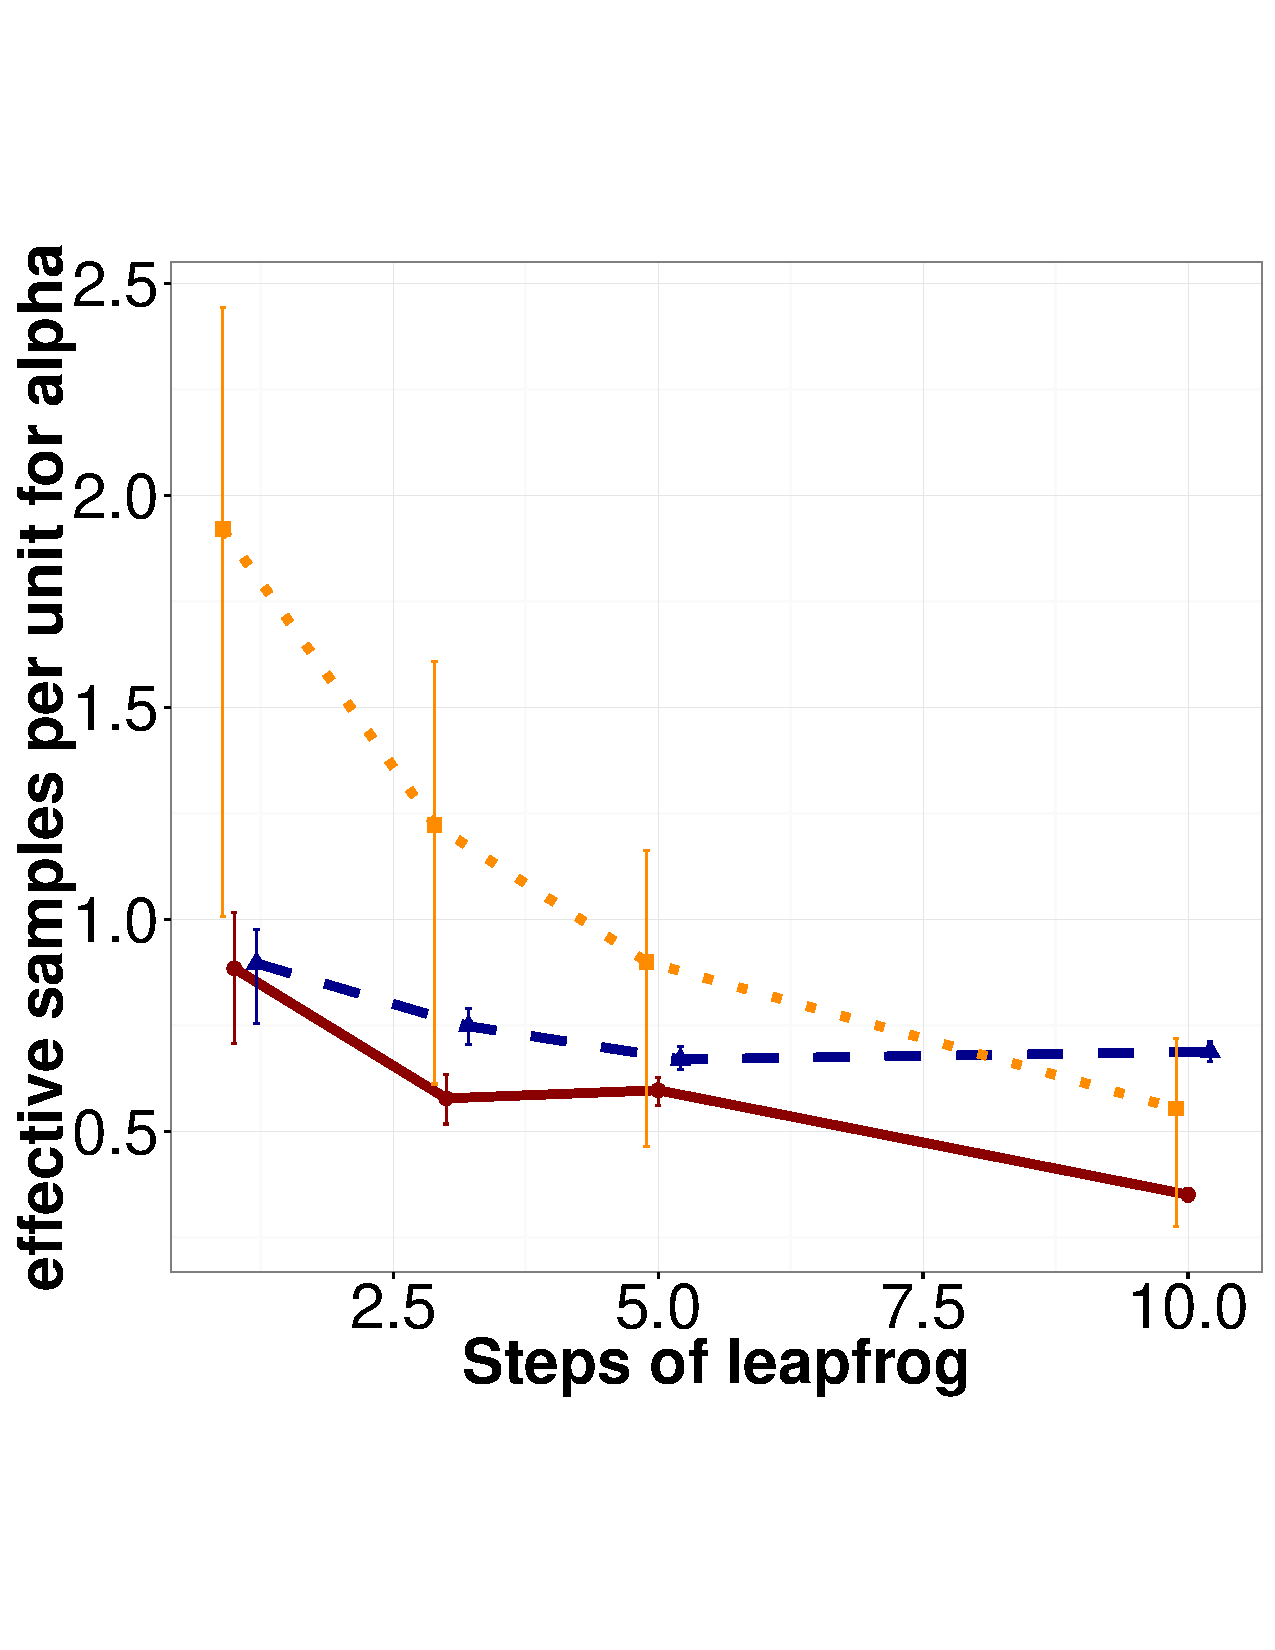
\includegraphics [width=0.90\textwidth, angle=0]{figs/h_alpha.pdf}
      \end{minipage}
  \begin{minipage}[hp]{0.45\linewidth}
  \centering
    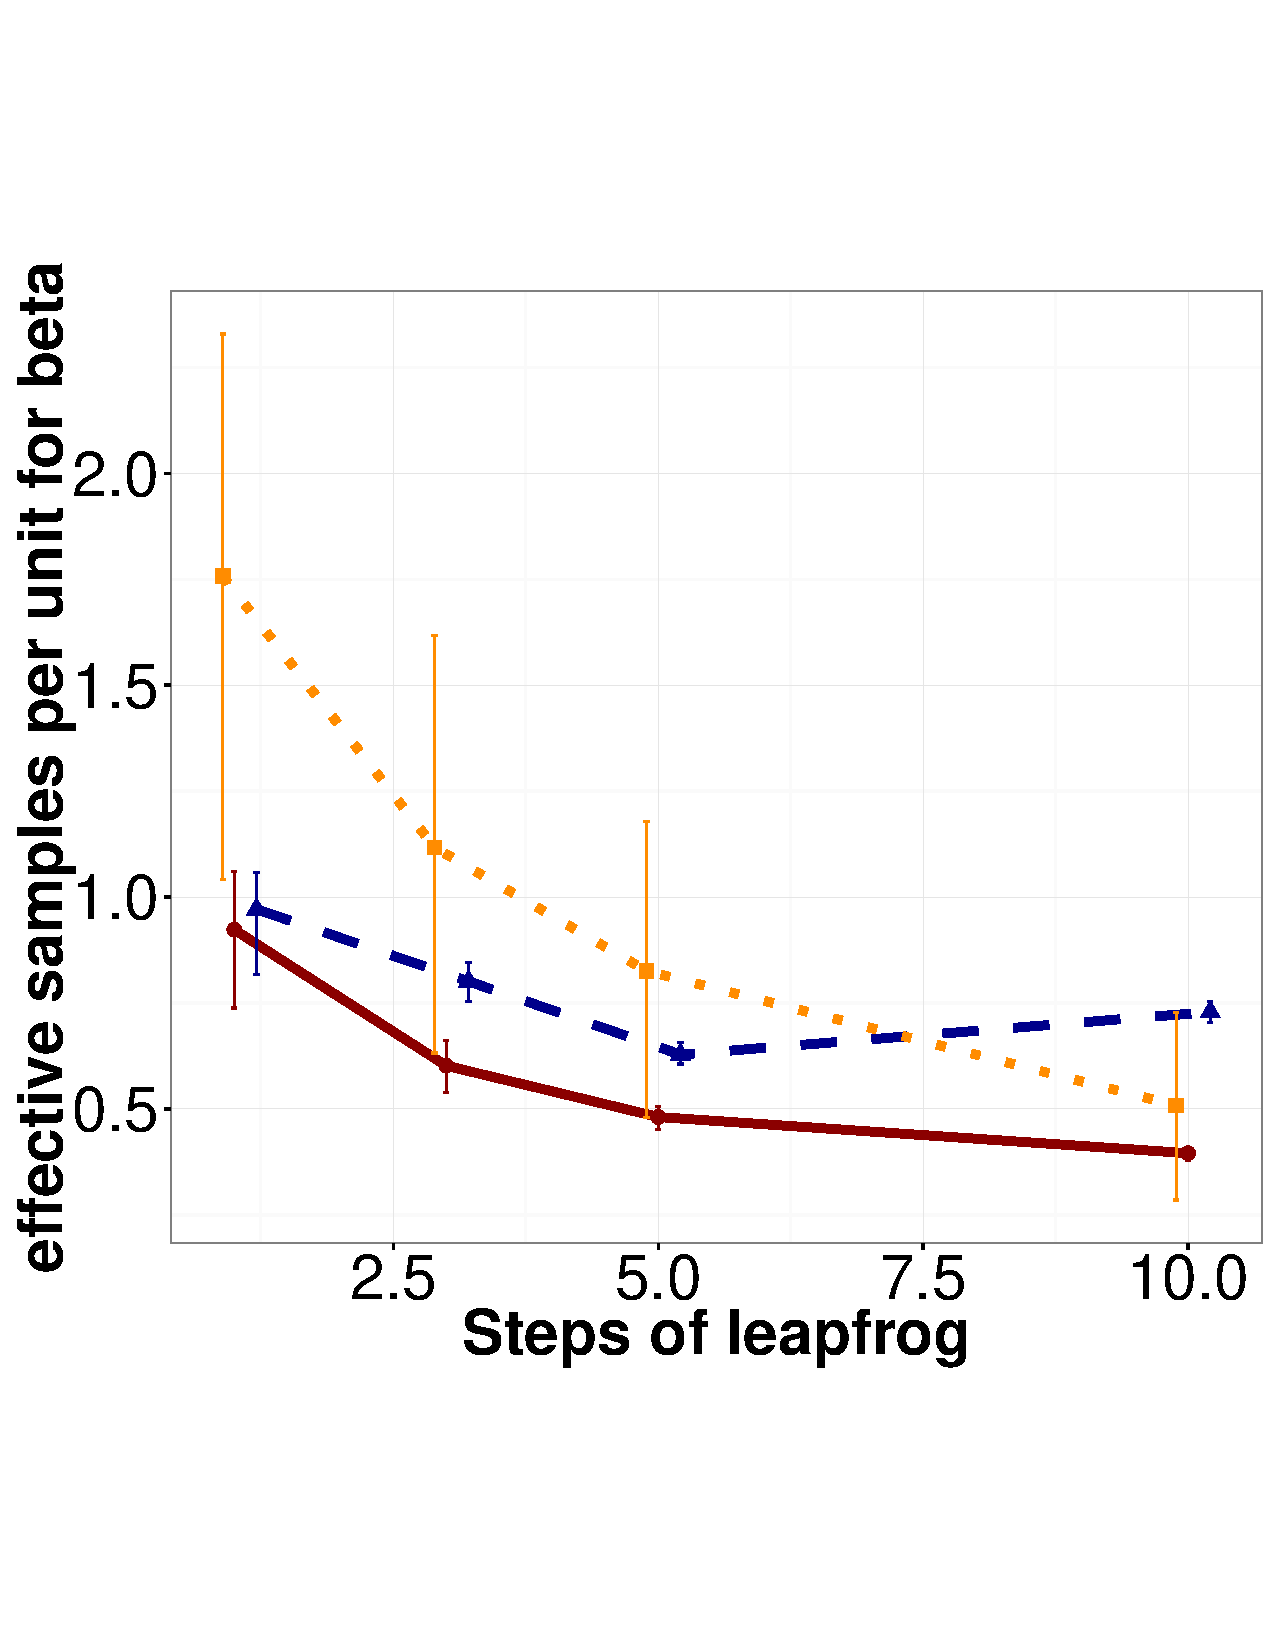
\includegraphics [width=0.90\textwidth, angle=0]{figs/h_beta.pdf}
      \end{minipage}
    \caption{HMC for dim 3}
    \label{fig:HMC_DIM_3}
  \end{figure}
In Figure~\ref{fig:HMC_DIM_3}, we plot the ESS per unit time as we change the 
number of leapfrog jumps in Hamiltonian MCMC for dimension $3$ for the 
immigration-death model. We consider 
three different step size for leapfrog step($s = 0.02, 0.05, 0.1$). 
% We use the same data for our previous experiment for the case when dimension $3$. 
We set the mass matrix $M$ to the identity matrix. We see that in this case,
the improved exploration afforded by HMC is not sufficient to overcome the 
computational burden it incurs: this is partly because every time a gradient is
computed (and this every leapfrog step), one needs to run the forward-backward algorithm.

  \begin{figure}[H]
  \centering
  \begin{minipage}[!hp]{0.45\linewidth}
  \centering
    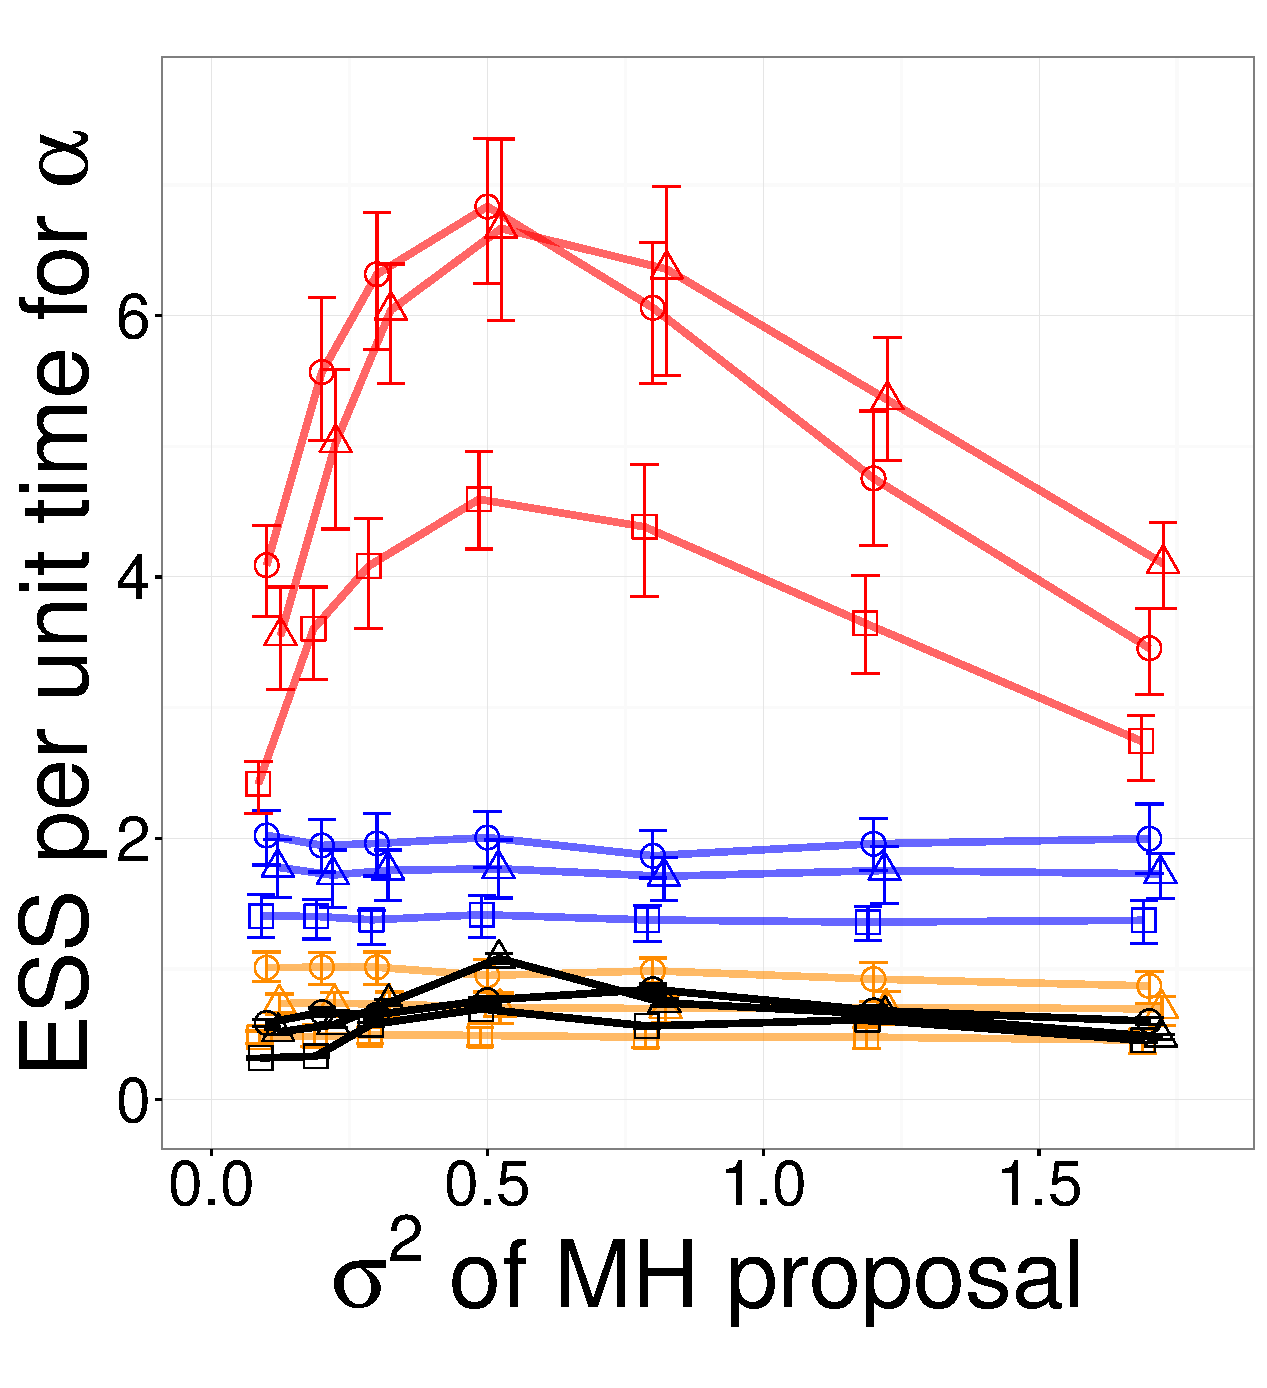
\includegraphics [width=0.90\textwidth, angle=0]{figs/exp_5_alpha.pdf}
      \end{minipage}
  \begin{minipage}[hp]{0.45\linewidth}
  \centering
    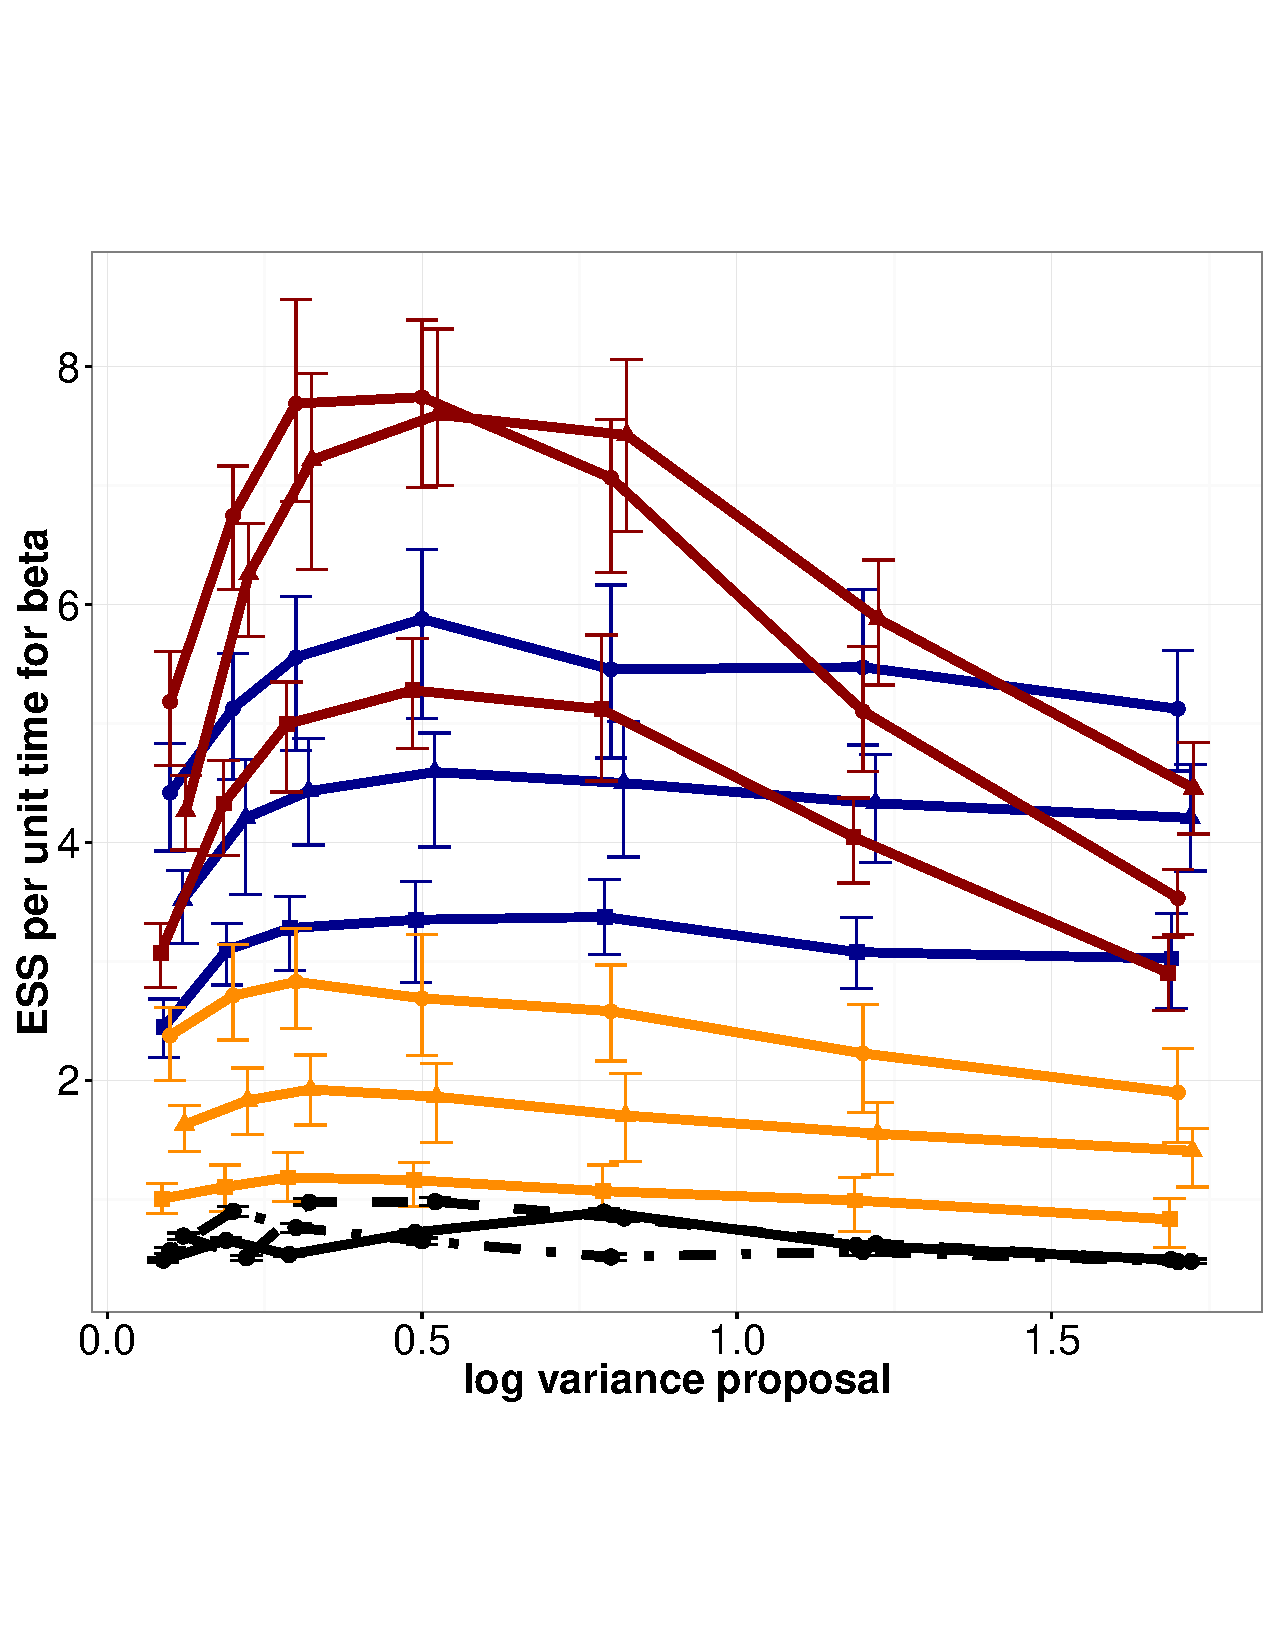
\includegraphics [width=0.90\textwidth, angle=0]{figs/exp_5_beta.pdf}
    \vspace{-0 in}
  \end{minipage}
    \caption{ESS/sec for the synthetic model with dimension 5. The left is for 
    $\alpha$, and the right is for $\beta$.}
     \label{fig:ESS_EXP_D5}
  \end{figure}

\subsection{Immigration model with capacity}
\begin{figure}[H]
  \begin{minipage}[hp]{0.85\linewidth}
  \centering
    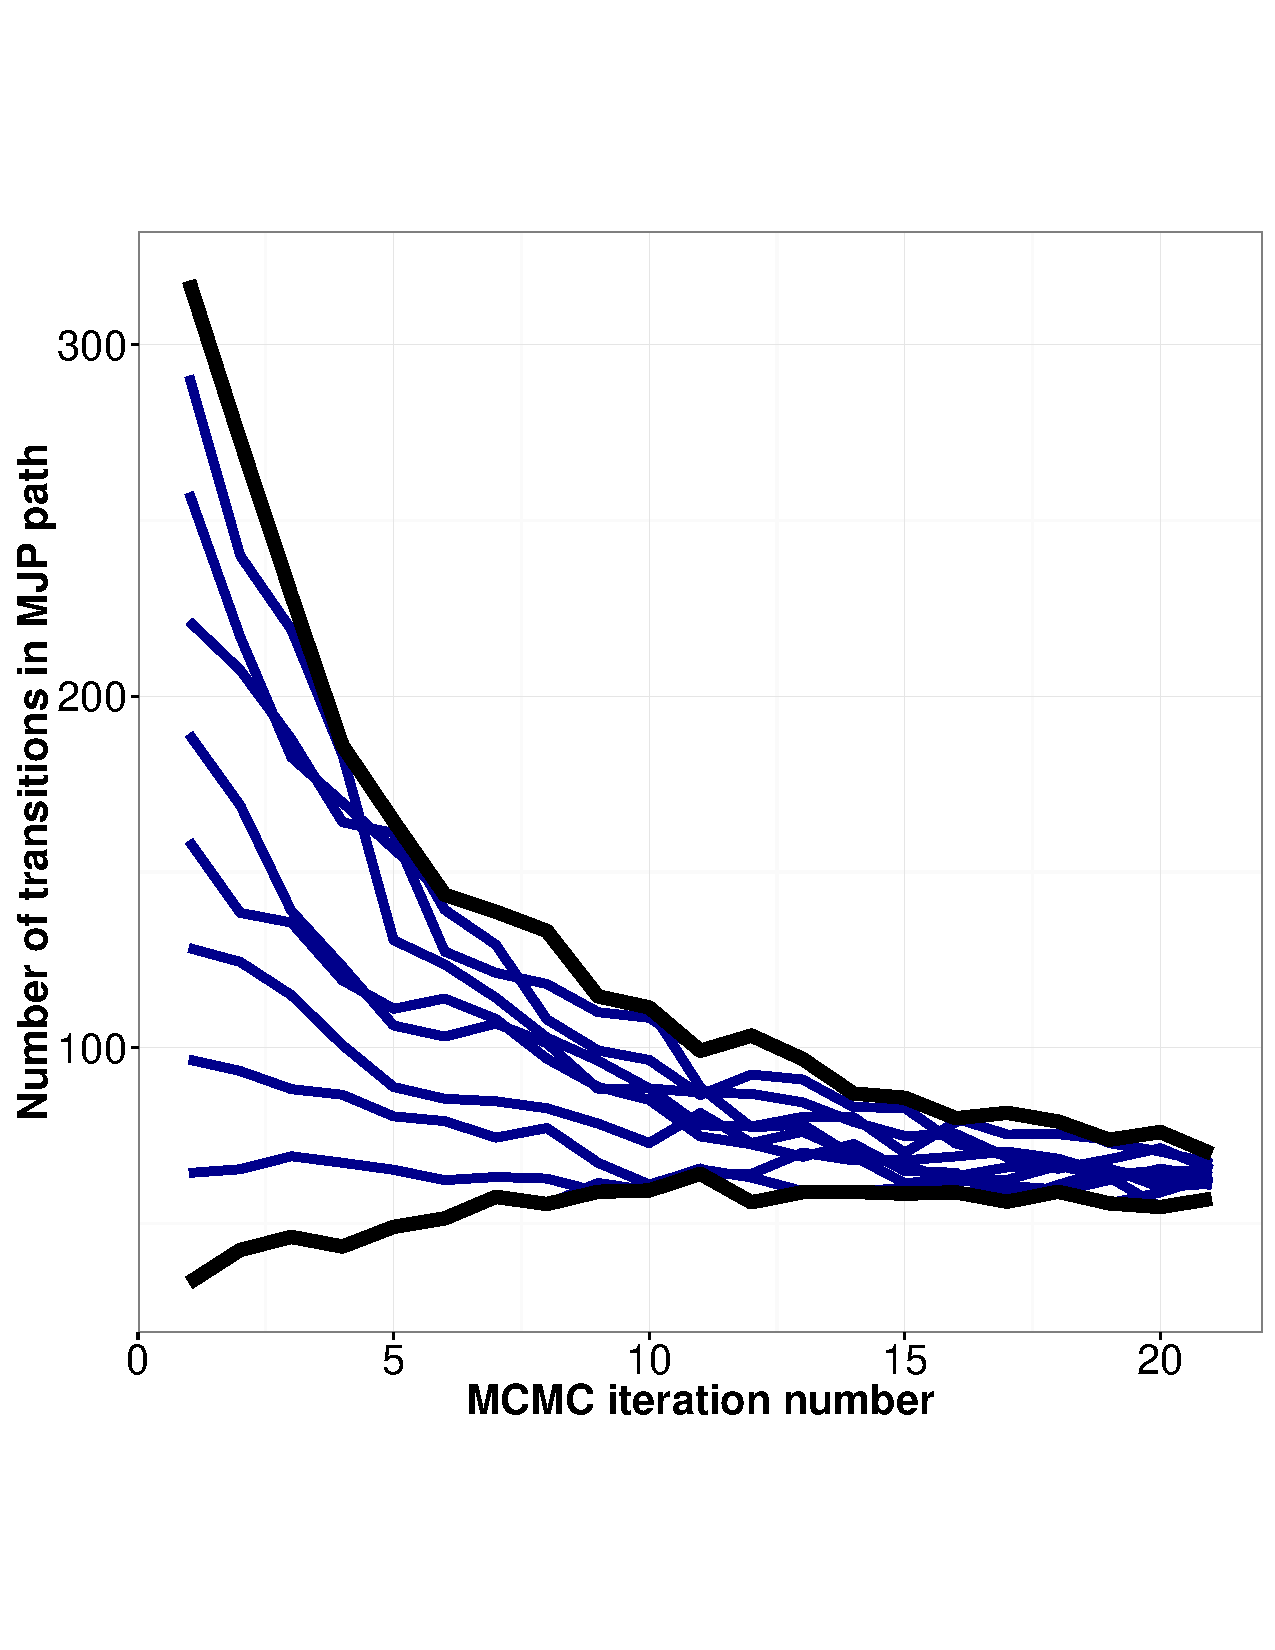
\includegraphics [width=0.40\textwidth, angle=0]{figs/q3_k2_path_transition.pdf}
    \vspace{-0 in}
    \caption{Trace plot of the number of MJP transitions for different initializatoins for immigration model.}
     \label{fig:ESS_Q_TRANSITION}
  \end{minipage}
\end{figure}

  \begin{figure}[H]
  \centering
  \begin{minipage}[hp]{0.45\linewidth}
  \centering
    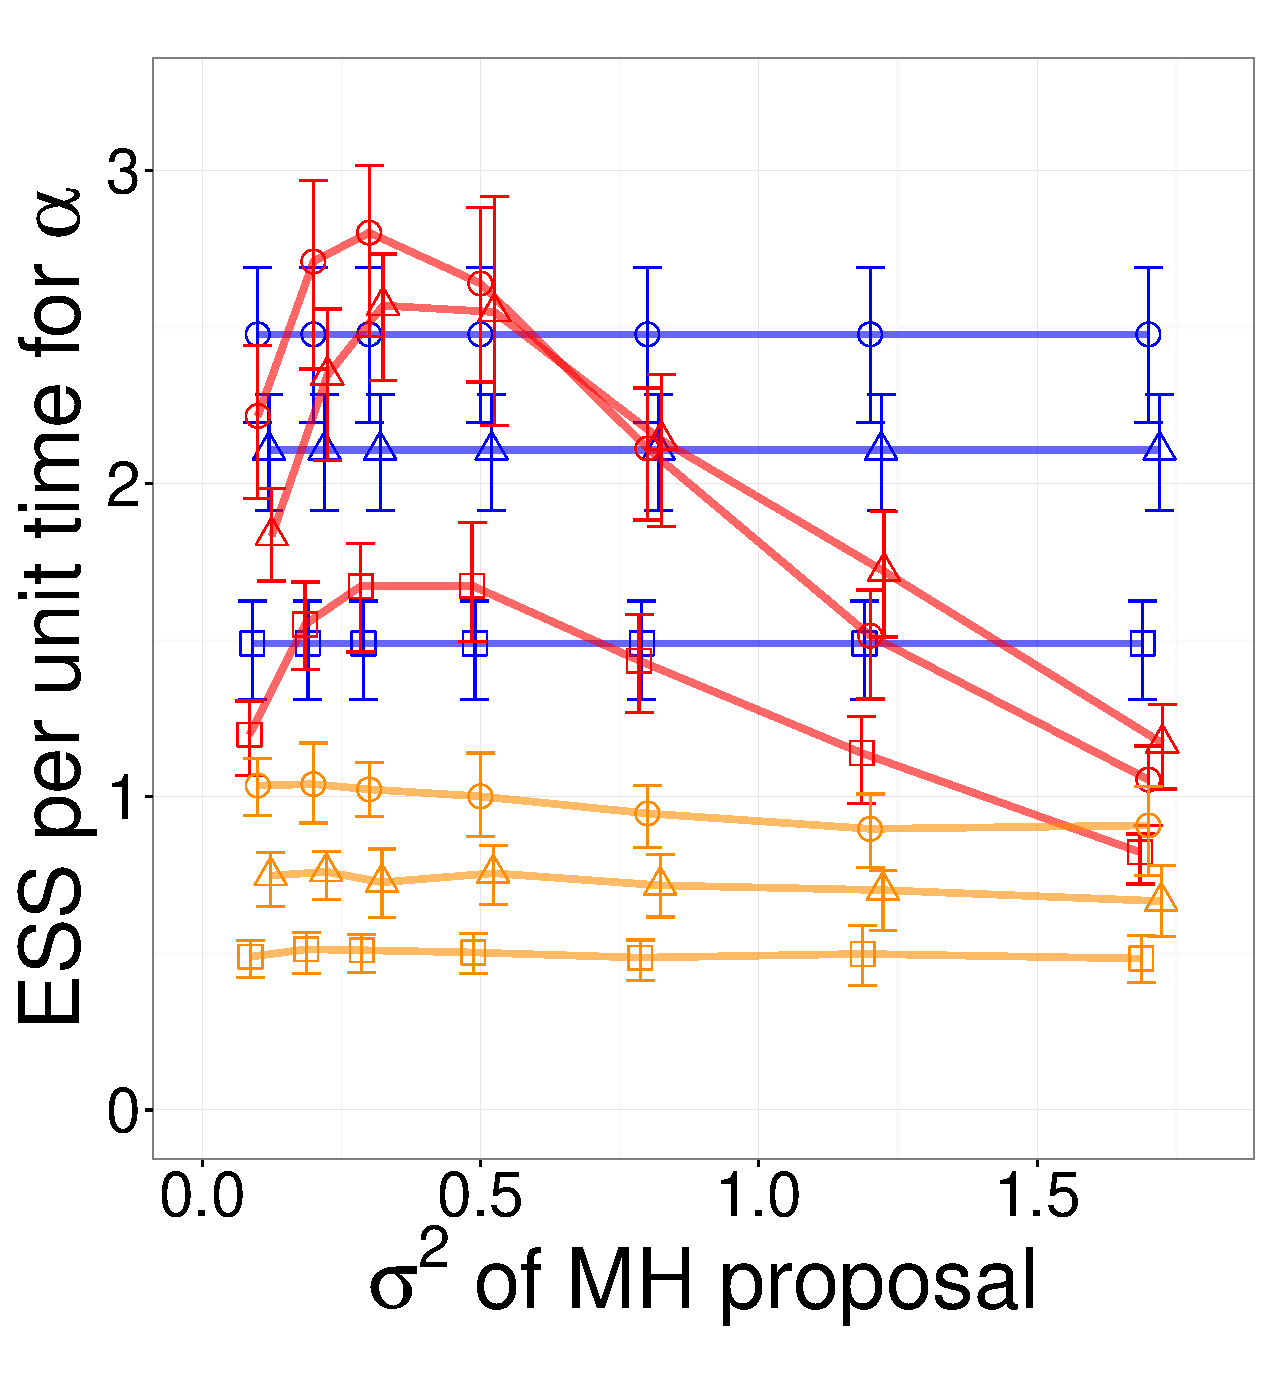
\includegraphics [width=0.90\textwidth, angle=0]{figs/q_5_alpha.pdf}
      \end{minipage}
  \begin{minipage}[hp]{0.45\linewidth}
  \centering
    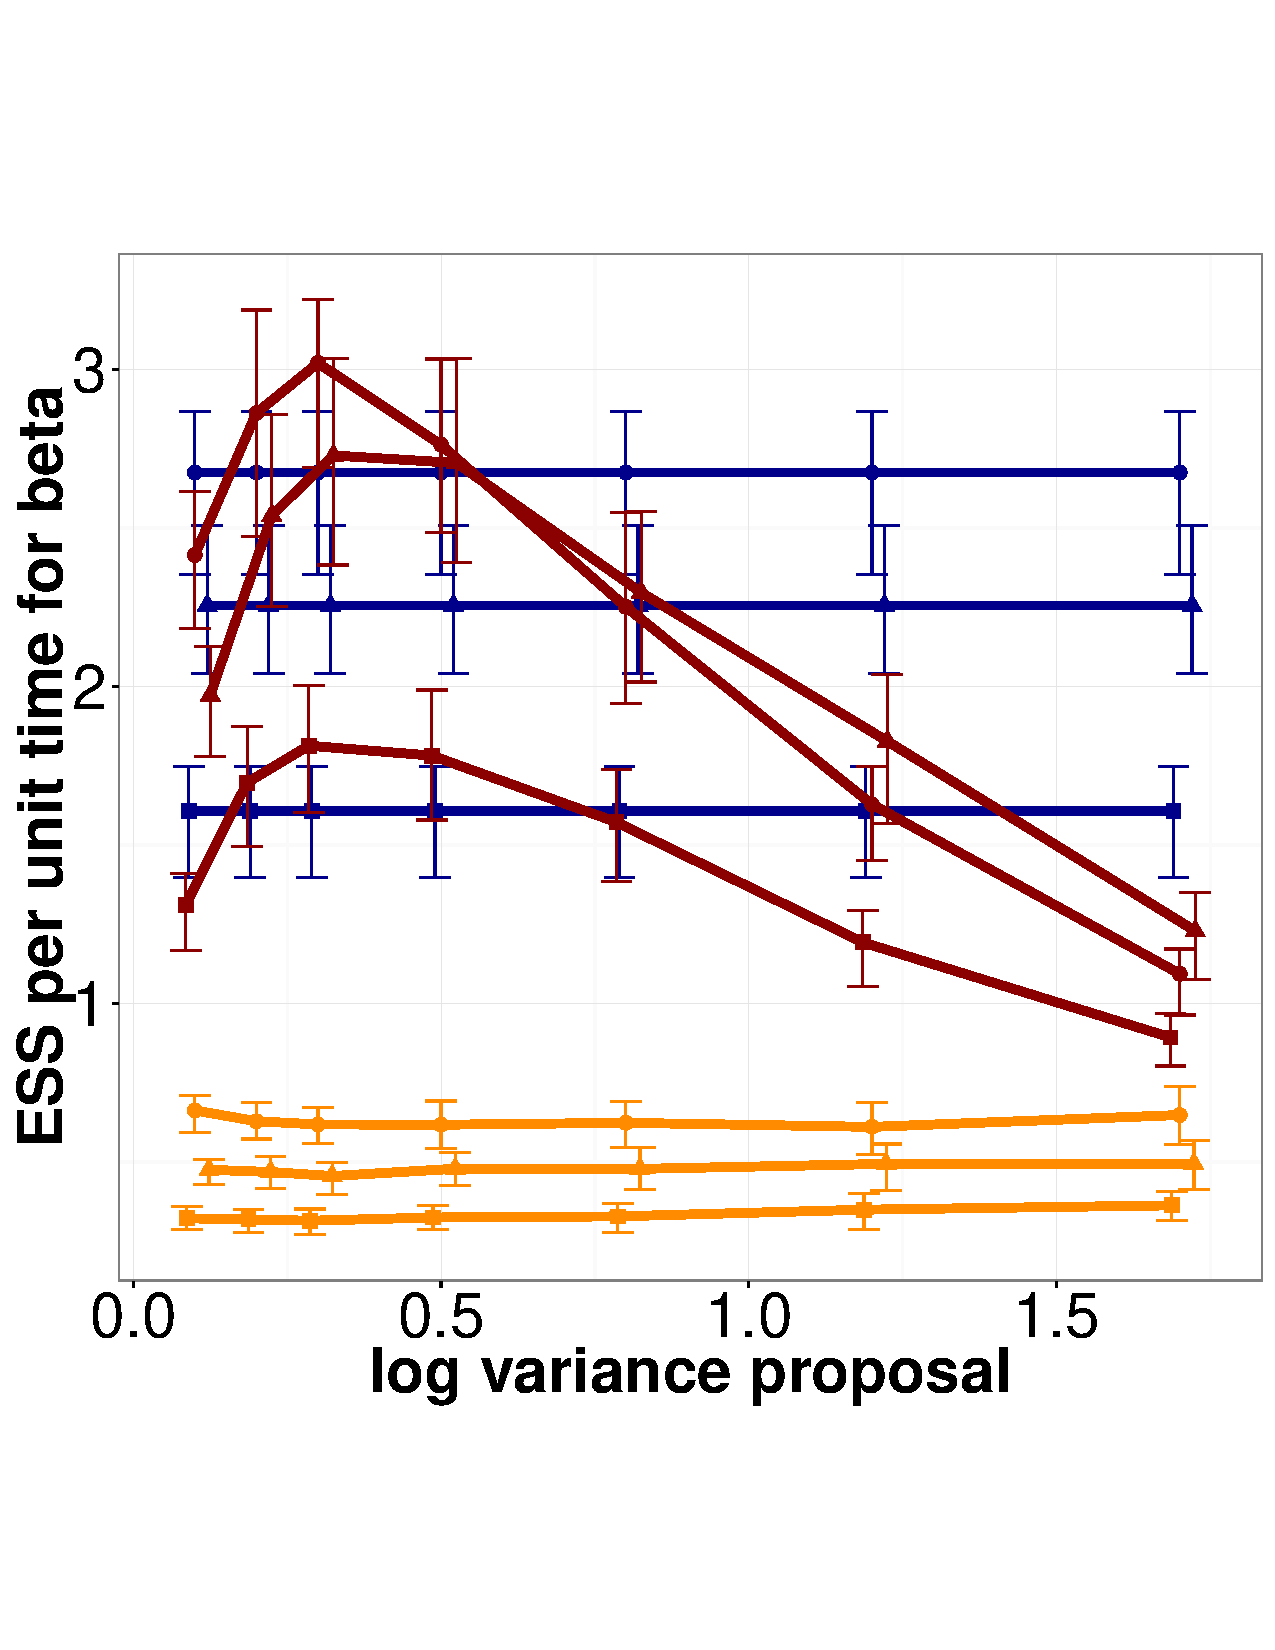
\includegraphics [width=0.90\textwidth, angle=0]{figs/q_5_beta.pdf}
    \vspace{-0 in}
      \label{fig:ESS_Q_D5}
  \end{minipage}
    \caption{ESS/sec for Immigration model (dim 5).The left is for $\alpha$, and the right is for $\beta$.}
  \end{figure}

\subsection{Non-homogeneous immigration model}

  \begin{figure}[H]
  \centering
  \begin{minipage}[!hp]{0.45\linewidth}
  \centering
    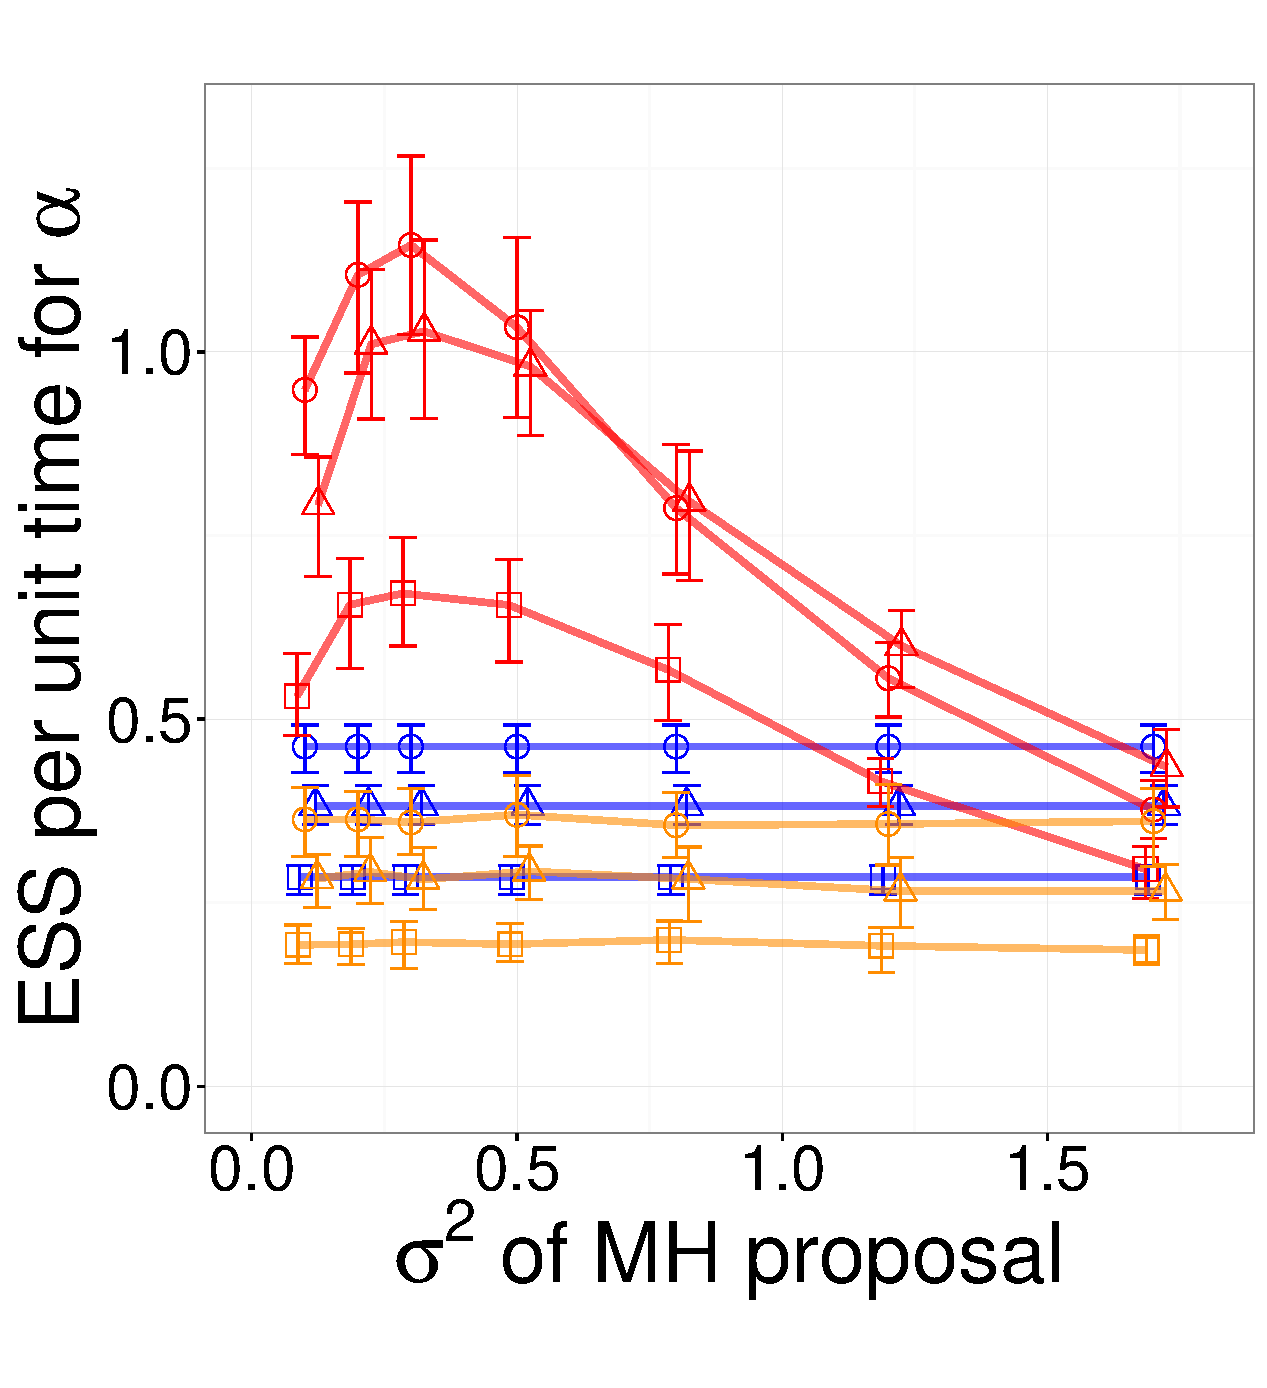
\includegraphics [width=0.950\textwidth, angle=0]{figs/pc_5_alpha.pdf}
      \end{minipage}
  \begin{minipage}[!hp]{0.45\linewidth}
  \centering
    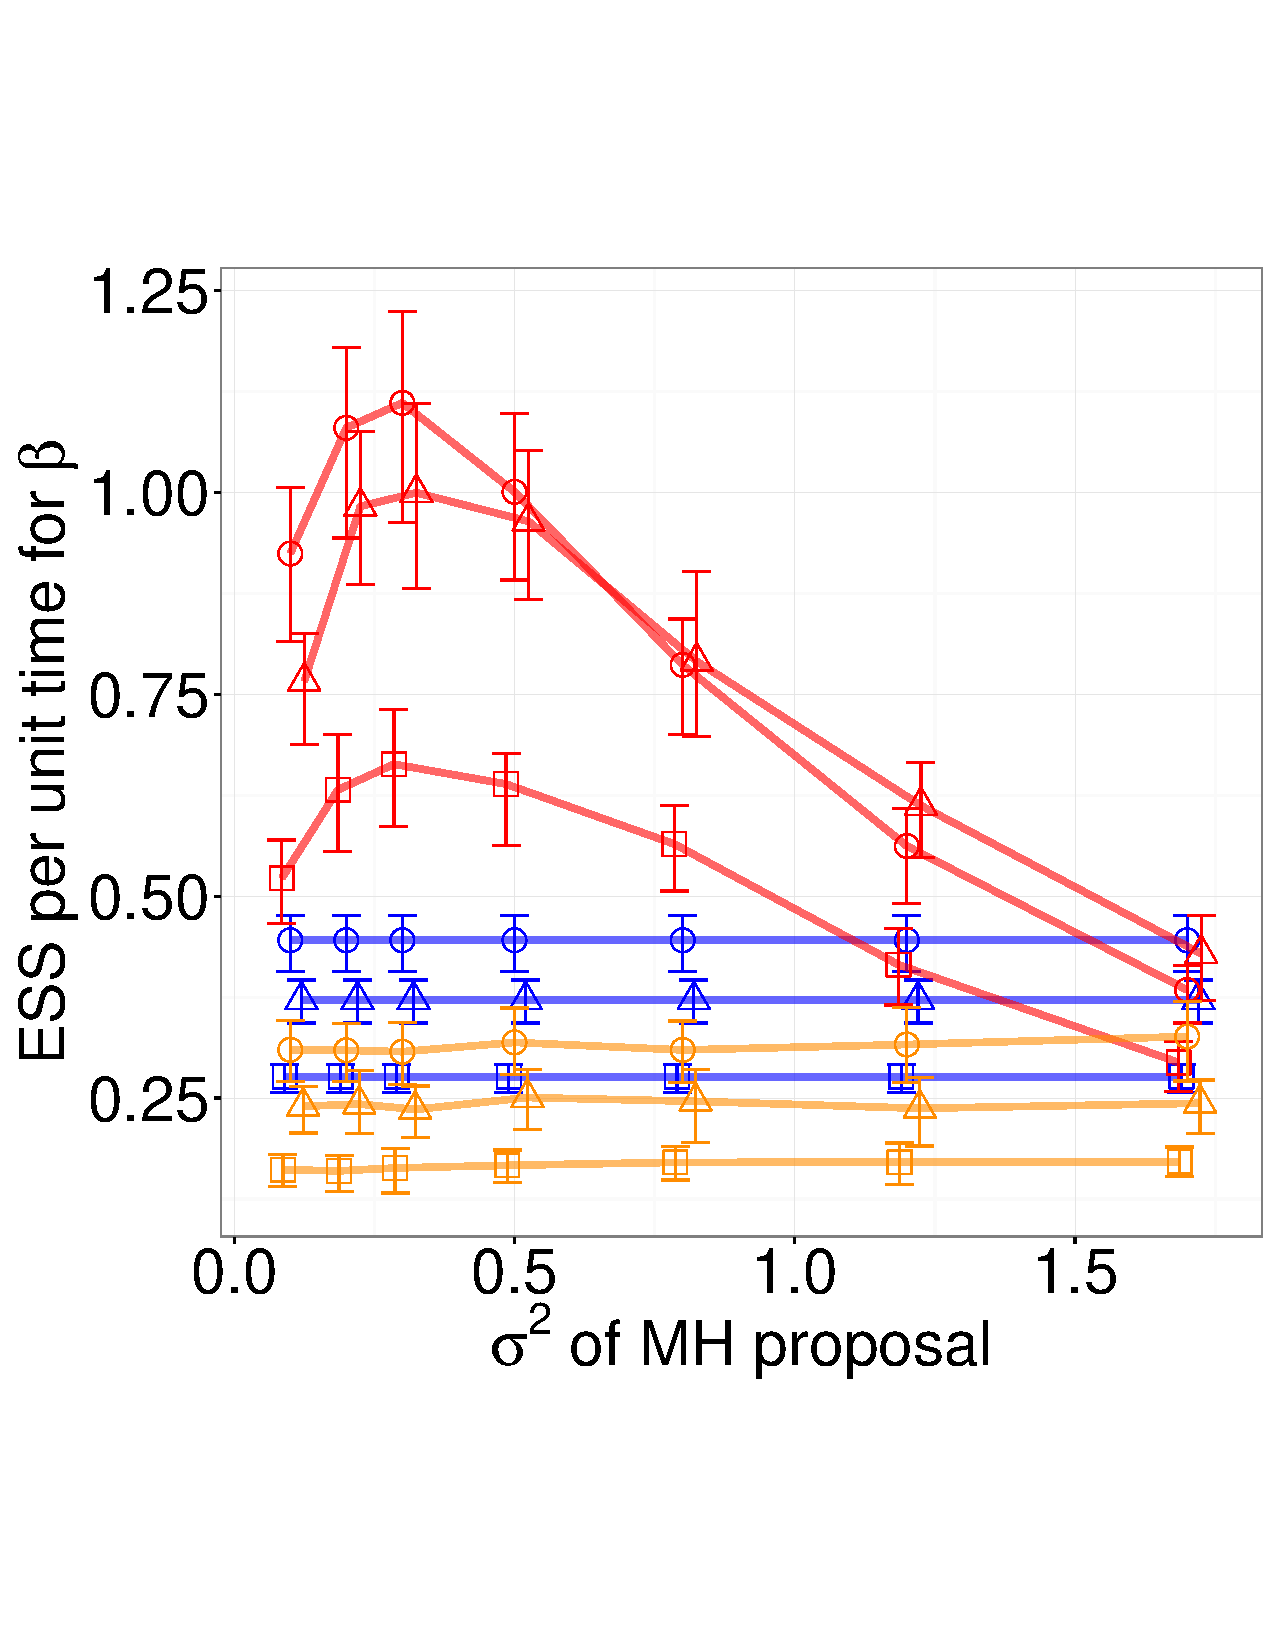
\includegraphics [width=0.950\textwidth, angle=0]{figs/pc_5_beta.pdf}
    \vspace{-0 in}
     \label{fig:ESS_pc_5}
  \end{minipage}
    \caption{ESS/sec for the nonhomogeneous immigration model (dim 5).The left is 
    for $\alpha$, and the right is for $\beta$.}
  \end{figure}

  \subsection{Immigration models with capacity}
  Below we include derivations of the posterior update rules for the immigration
  model with capacity.

  \noindent Assume our current state consists of a trajectory $S(t) \equiv (S,T)$,
  with: $S = [S_0,S_1, ...,S_n] \;, T = [t_0(t_{start}), t_1,...,t_n, t_{n+1}(t_{end})]$, and $y$ as observations.\\
Recall the definition of the immigration model. The state space is 
$\{0, 1, 2, ..., N - 1 \}$, representing the total population. The transition matrix is defined as follows. 
\begin{align*}
&-A_i =: A_{i,i} = -(\alpha + i\beta), \; \; i =0,1,...,N - 1 ;\\
&A_{i, i+1} = \alpha, \; \; i =0,1,...,N-2;\\
&A_{i, i-1}  = \beta, \; \;  i =1,...,N - 1.
\end{align*} And all the other elements are $0$.
%$$A_i =: A_{i,i} = -(\alpha + i\beta), \; \; i =0,1,...,N$$ $$A_{i, i+1} = \alpha, \; \; i =0,1,...,N-1,$$ $$A_{i, i-1}  = \beta, \; \;  i =1,...,N.$$
The conditional density(given $\alpha,\; \beta$) of a MJP trajectory $(s_0, S, T)$ in time interval $[t_{start}, t_{end}]$, with $S=(s_1, s_2,..., s_n)$, $T=(t_1, t_2,..., t_n)$ is 
$$f(s_0,S,T| \alpha, \beta) = \prod_{i=0}^{n-1} A_{s_i, s_{i+1}} \exp(\sum_{i=0}^{n} A_{s_i}(t_{i+1} - t_{i})).$$
%where $t_0 = t_{start}$, $t_{n+1} = t_{end}.$\\
%Let's denote some notations here.\\
Define
\begin{align*}
&U(s_0, S, T):= \sum_{i=0}^{n-1} \mathbb{I}_{\{s_{i+1} - s_i = 1\}} ; \\
&D(s_0, S, T):= \sum_{i=0}^{n-1} \mathbb{I}_{\{s_{i+1} - s_i = -1\}}.
\end{align*}
%$$U(s_0, S, T):= \sum_{i=0}^{k-1} \mathbb{I}_{\{s_{i+1} - s_i = 1\}}.$$
%$$D(s_0, S, T):= \sum_{i=0}^{k-1} \mathbb{I}_{\{s_{i+1} - s_i = -1\}}.$$
Let us call them U and D for short. Denote the total time when the trajectory state stays at state i as $\tau_i$, i.e. $\tau_i = \sum_{j=0}^{n} (t_{j+1} -t_j)\mathbb{I}_{\{s_j = i\}}$, then $\sum_{i=0}^n (t_{i+1} - t_i)s_i = \sum_{i=0}^{N - 1} \tau_ii.$
$$f(s_0,S,T| \alpha, \beta) = \exp(-\alpha(t_{end} - t_{start}- \tau_N) )\alpha^U \cdot  \exp((-(\sum_{i=0}^k (t_{i+1} - t_i)s_i)\beta) \prod_{i=1}^{N - 1} i^{\sum_{j=0}^{k-1}\mathbb{I}_{s_{j+1} = i -1 \;,  s_j = i} }   \beta^D$$\\
We place Gamma$(\mu, \lambda)$ and Gamma$(\omega,  \theta)$ priors on the parameters $\alpha$ and $\beta$,
%If we assume the prior of $\alpha$, and $\beta$ are $Gamma(\mu,\lambda)$, $Gamma(\omega, \theta)$, which are independent with each other. \\
%$$p(\alpha) = \frac{\lambda^\mu}{\Gamma(\mu)}\alpha^{\mu -1}e^{-\lambda \alpha}. $$
%$$p(\beta) = \frac{\theta^\omega}{\Gamma(\omega)}\beta^{\omega -1}e^{-\theta \beta}. $$
and then the posterior distribution $f(\alpha, \beta | s_0,S,T)$ is as follows:
$$ f(\alpha, \beta | s_0,S,T) \propto \exp(-(\lambda + t_{end} - t_{start}- \tau_{N - 1})\alpha) \alpha^{\mu + U -1} \cdot \exp(-(\sum_{i=0}^n (t_{i+1} - t_i)s_i + \theta)\beta) \beta^{\omega+ D -1}.$$
Thus, the posterior distributions of $\alpha$, $\beta$ are still independent. In
particular,
\begin{itemize}
\item $\alpha | s_0,S,T$ is $Gamma(\mu+ U,\lambda + t_{end} - t_{start}- \tau_{N - 1})$ distributed\\
\item $\beta | s_0,S,T$ is $Gamma(\omega+ D,\theta + \sum_{i=0}^n (t_{i+1} - t_i)s_i)$ distributed, which is equivalent to $Gamma(\omega+ D,\theta +\sum_{i=0}^{N - 1} \tau_ii)$\\
\end{itemize}
Such immigration models have perfectly conjugate posterior distributions when we 
assign Gamma priors to $\alpha$ and $\beta$. 

\end{document}
